\documentclass[12pt, a4paper]{article}

\usepackage[top=2.5cm, bottom=2.5cm, left=3cm, right=3cm]{geometry}
\usepackage{mdframed}
\usepackage[utf8]{inputenc}
\usepackage[T1]{fontenc}
\usepackage[spanish]{babel}
\usepackage{amsmath}
\usepackage{float}
\usepackage[margin=10pt, font=small, labelfont=bf]{caption}
\usepackage{booktabs}
\usepackage{graphicx}
\usepackage{xcolor}
\usepackage{hyperref}
\usepackage{longtable}
\usepackage{comment}
\usepackage{setspace}
\usepackage{titlesec}
\usepackage{fancyhdr}
\usepackage{threeparttable}

\setlength{\textfloatsep}{18pt plus 2pt minus 4pt}
\setlength{\floatsep}{12pt plus 2pt minus 2pt}
\setlength{\intextsep}{14pt plus 2pt minus 2pt}
\setstretch{1.15}
\setlength{\parindent}{0pt}
\setlength{\parskip}{8pt}

\titleformat{\section}
  {\large\bfseries}{\thesection.}{0.5em}{}
  [\vspace{2pt}\hrule\vspace{4pt}]
\titleformat{\subsection}
  {\normalsize\bfseries}{\thesubsection.}{0.5em}{}
\titlespacing{\section}{0pt}{18pt}{8pt}
\titlespacing{\subsection}{0pt}{14pt}{6pt}

\hypersetup{colorlinks=true, linkcolor=blue!60!black}

\pagestyle{fancy}
\fancyhf{}
\fancyhead[L]{\footnotesize Centro Javeriano de Competitividad}
\fancyhead[R]{\footnotesize \reportnumber}
\cfoot{\thepage}
\setlength{\headheight}{14pt}
\renewcommand{\headrulewidth}{0.4pt}

\geometry{margin=1in}
\graphicspath{{Paper/figures/}{figures/}}
\newcommand{\tablepath}{Paper/tables/}
\newcommand{\figurelang}{es}
\newcommand{\reportseries}{Informes sobre la Productividad en Colombia}
\newcommand{\reportseriesdesc}{Evidencia para entender y fomentar la productividad}
\newcommand{\reportnumber}{Informe 0X}
\newcommand{\reporttitle}{Remuneración Laboral por Logro Educativo en Colombia 2010--2025}
\newcommand{\reportsubtitle}{Una lectura a partir de la GEIH}
\newcommand{\reportauthorone}{Oliver Pardo}
\newcommand{\reportauthoroneaffil}{Profesor asociado del Departamento de Administración, Pontificia Universidad Javeriana y Director del Centro Javeriano de Competitividad}
\newcommand{\reportauthortwo}{Jorge Orozco}
\newcommand{\reportauthortwoaffil}{Consultor de investigación del Centro Javeriano de Competitividad, Pontificia Universidad Javeriana}
\renewcommand{\contentsname}{Tabla de contenido}

\title{\reporttitle\\\reportsubtitle}
\author{\reportauthorone \and \reportauthortwo}
\date{\today}

\begin{document}

\begin{titlepage}
\thispagestyle{empty}
\vspace*{0.6cm}

\begin{center}

\includegraphics[width=0.58\textwidth]{logo_cjc_palatino_horizontal.png}
\end{center}

\vspace{1.5cm}

\begin{center}
{\Large\bfseries \reportseries\par}
\vspace{0.15cm}
{\large \reportseriesdesc\par}

\vspace{1.4cm}

{\large\bfseries \reportnumber\par}
\vspace{0.45cm}
{\Huge\bfseries \reporttitle\par}
%\vspace{0.35cm}
%{\Large \reportsubtitle\par}
\vspace{0.65cm}
%{\large\bfseries \reportauthorone\par}
%{\normalsize \reportauthoroneaffil\par}
%\vspace{0.25cm}
%{\large\bfseries \reportauthortwo\par}
%{\normalsize \reportauthortwoaffil\par}
\end{center}

\vfill

\begin{center}
{\large \today\par}
\end{center}

\end{titlepage}

\begin{mdframed}[
  linewidth=1pt,
  linecolor=gray!60,
  backgroundcolor=gray!6,
  innertopmargin=12pt,
  innerbottommargin=12pt,
  innerleftmargin=14pt,
  innerrightmargin=14pt
]
\section*{Resumen ejecutivo}
\addcontentsline{toc}{section}{Resumen ejecutivo}
\textbf{Este informe examina la evolución de la remuneración laboral en Colombia entre 2010 y 2025 y cómo esta se relaciona con los niveles de logro educativo de la población ocupada.} Para ello, los trabajadores se agrupan según su máximo nivel educativo alcanzado: primaria o menos, educación secundaria o media, y educación superior. El análisis compara la trayectoria de sus ingresos a lo largo del tiempo, considerando tanto la remuneración mensual como la remuneración por hora trabajada.

\textbf{En 2025, los trabajadores con educación superior percibieron una remuneración promedio 3,2 veces mayor que la de quienes contaban con educación primaria o menos.} En términos mensuales, sus ingresos alcanzaron en promedio 3,2 millones de pesos de 2025, frente a 1,0 millón entre quienes tenían un menor nivel educativo. Esta diferencia también se refleja en la remuneración por hora trabajada, que fue de 17,2 mil pesos para las personas con educación superior y de 5,4 mil pesos para aquellas con primaria o menos.

\textbf{El nivel educativo de la población ocupada aumentó de manera significativa entre 2010 y 2025, contribuyendo al crecimiento de la remuneración promedio por trabajador.} Durante este período, la participación de personas con educación superior dentro de la población ocupada pasó de 23\% a 34\%, mientras que la de quienes tenían educación primaria o menos se redujo de 36\% a 21\%. Este cambio en la composición educativa de la fuerza laboral favoreció un aumento de los ingresos promedio, dado que los trabajadores con mayores niveles de educación tienden a percibir remuneraciones más elevadas.

\textbf{Sin embargo, la remuneración de los trabajadores con educación superior registró un crecimiento moderado durante el período analizado.} Entre 2010 y 2025, la remuneración mensual de este grupo aumentó apenas 0,3\% anual, mientras que la remuneración por hora creció 0,5\% por año. Como resultado, los ingresos asociados a cada nivel educativo avanzaron a un ritmo menor que la remuneración promedio por trabajador, cuyo crecimiento estuvo impulsado principalmente por el aumento del nivel educativo de la población ocupada.

\textbf{Entre 2021 y 2025, la remuneración aumentó para quienes alcanzaron doctorado, maestría, formación tecnológica o formación técnica profesional.} Para quienes alcanzaron pregrado universitario o especialización, en cambio, la remuneración cayó o se mantuvo estancada.

%\textbf{Entre 2021 y 2025, el crecimiento de la remuneración fue heterogéneo entre los distintos niveles de educación superior.} Mientras que los trabajadores con doctorado, maestría, formación tecnológica o formación técnica profesional experimentaron aumentos en sus ingresos, aquellos con pregrado universitario o especialización enfrentaron una reducción de la remuneración o una trayectoria prácticamente estancada.
\end{mdframed}

\newpage
\tableofcontents
\newpage

\section{Introducción}\label{sec:introduccion}

\textbf{En Colombia, los años de formación suelen traducirse en un mejor acceso a oportunidades laborales y mayores ingresos.} Alcanzar niveles educativos más altos está asociado con un conjunto más amplio de conocimientos y habilidades, lo que se refleja en una mayor productividad por hora trabajada. A su vez, los empleadores están dispuestos a remunerar mejor a aquellos trabajadores que aportan más valor a los procesos productivos. Por esta razón, una mayor acumulación de capital humano suele ir acompañada de mejores condiciones salariales.

\textbf{La remuneración se utiliza en este informe como una aproximación, mas no como una medida directa, de la productividad marginal del trabajo.} Este concepto hace referencia al valor adicional que genera una empresa al incorporar una unidad adicional de trabajo. En un mercado laboral competitivo, sin asimetrías de información y con remuneraciones plenamente flexibles, la contratación tiende a realizarse hasta el punto en que el costo de una hora adicional de trabajo se iguala con el valor de lo que esa hora produce. Bajo estas condiciones, la remuneración por hora coincide con la productividad marginal del trabajador. Sin embargo, en la práctica los salarios también reflejan otros factores, como el poder de negociación entre empleadores y trabajadores, la existencia de rigideces institucionales —entre ellas el salario mínimo—, los incentivos que buscan generar las empresas y las fricciones propias de la búsqueda de empleo. Por ello, los resultados sobre cambios en la remuneración deben interpretarse con cautela cuando se utilizan como indicio de variaciones en la productividad. Esta advertencia resulta especialmente relevante en el período posterior a la pandemia, cuando los aumentos salariales coincidieron con incrementos significativos del salario mínimo.


\textbf{El objetivo de este informe es analizar cómo ha evolucionado la remuneración laboral según el nivel educativo alcanzado entre 2010 y 2025.} Para ello, se clasifica a la población ocupada con base en la información reportada en la Gran Encuesta Integrada de Hogares (GEIH), distinguiendo entre quienes tienen educación primaria o menos, educación secundaria o media y educación superior. A partir de esta clasificación, se estudia la evolución de los ingresos laborales tanto en términos de remuneración mensual por trabajador como de remuneración por hora trabajada.

\textbf{El crecimiento de la remuneración promedio por trabajador puede explicarse por cambios en la composición educativa de la población ocupada o por mejoras en la remuneración asociada a cada nivel educativo.} La remuneración promedio de los trabajadores puede entenderse como el promedio de las remuneraciones de cada grupo educativo, ponderadas por la participación de cada uno dentro de la población ocupada. En consecuencia, existen dos mecanismos a través de los cuales este indicador puede aumentar. El primero es que una proporción creciente de trabajadores alcance niveles educativos más altos y acceda a empleos mejor remunerados. El segundo es que aumente la remuneración de quienes pertenecen a cada nivel educativo, reflejando mejoras en su productividad o en las condiciones del mercado laboral.

\textbf{Los resultados sugieren que el aumento de la remuneración promedio por trabajador estuvo impulsado principalmente por el mayor nivel educativo de la población ocupada.} Si bien alcanzar educación superior continúa asociado con ingresos significativamente más altos, los avances en productividad no pueden depender únicamente de que más personas accedan a este nivel de formación. También resulta necesario promover aumentos sostenidos en la remuneración de los trabajadores dentro de cada nivel educativo, de manera que las mejoras en capital humano se traduzcan en mayores ingresos para toda la fuerza laboral.

\textbf{El informe está organizado en cinco secciones, incluyendo esta introducción.} La Sección \ref{sec:metodologia} describe las medidas de remuneración laboral estudiadas, la correspondencia entre logros educativos a lo largo del periodo estudiado y la descomposición del crecimiento de la remuneración entre el mayor logro educativo de la población ocupada y la remuneración de cada logro educativo. La Sección \ref{sec:grupos_comparables} presenta la dinámica de la remuneración entre 2010 y 2025 para quienes cuentan con primaria o menos, secundaria o media y superior o universitaria. La Sección \ref{sec:categorias_detalladas} aprovecha la apertura de la pregunta educativa desde 2021 para mirar la evolución de la remuneración para logros educativos más desagregados. Finalmente, la Sección \ref{sec:conclusiones} resume los retos de la educación dentro de la agenda nacional de productividad.

\section{Metodología}\label{sec:metodologia}

\subsection{Medición}

\textbf{El informe calcula la remuneración laboral a partir de la Gran Encuesta Integrada de Hogares (GEIH) para 2010--2025.} A partir de los ingresos laborales devengados el último mes y las horas trabajadas la última semana se construyen dos medidas: la remuneración mensual por trabajador y la remuneración por hora trabajada. Ambas se expresan en pesos constantes de 2025. 

\textbf{Los trabajadores se clasifican según el mayor logro educativo reportado en la GEIH.} Esta variable permite identificar el logro educativo alcanzado por cada ocupado, pero sus respuestas no son idénticas en todo el periodo. Antes de 2021, la encuesta ofrecía seis respuestas válidas: ninguno, preescolar, básica primaria, básica secundaria, media y superior o universitaria. Desde 2021, conserva las primeras cuatro respuestas, separa media en media académica y media técnica, y desagrega la respuesta superior o universitaria en normalista, técnica profesional, tecnológica, universitaria, especialización, maestría y doctorado.

\textbf{Para construir una serie comparable, el informe homologa esas respuestas en tres logros educativos.} Primaria o menos agrupa ninguno, preescolar y básica primaria. Secundaria o media agrupa básica secundaria y media, incluyendo media académica y media técnica desde 2021. Superior o universitaria agrupa las respuestas que antes aparecían como superior o universitaria y, desde 2021, las credenciales posteriores a la media. El Cuadro \ref{tab:mapeo_logros_educativos} resume esta homologación.

\begin{table}[H]
\centering
\caption{Correspondencia entre logros educativos}
\label{tab:mapeo_logros_educativos}
\footnotesize
\setlength{\tabcolsep}{4pt}
\begin{tabular}{@{}p{4.2cm}p{4.2cm}p{4.2cm}@{}}
\toprule
Agregación & Respuestas antes de 2021 & Respuestas desde 2021 \\
\midrule
Primaria o menos & Ninguno & Ninguno \\
Primaria o menos & Preescolar & Preescolar \\
Primaria o menos & Básica primaria & Básica primaria \\
Secundaria o media & Básica secundaria & Básica secundaria \\
Secundaria o media & Media & Media académica \\
Secundaria o media & Media & Media técnica \\
Superior o universitaria & Superior o universitaria & Normalista \\
Superior o universitaria & Superior o universitaria & Técnica profesional \\
Superior o universitaria & Superior o universitaria & Tecnológica \\
Superior o universitaria & Superior o universitaria & Universitaria \\
Superior o universitaria & Superior o universitaria & Especialización \\
Superior o universitaria & Superior o universitaria & Maestría \\
Superior o universitaria & Superior o universitaria & Doctorado \\
\bottomrule
\end{tabular}
\caption*{\footnotesize Nota: la agregación permite mantener una clasificación comparable entre 2010 y 2025. La opción \textit{No sabe, no informa} no se asigna a ningún logro educativo. Fuente: clasificación propia a partir de la variable de logro educativo de la GEIH.}
\end{table}

\subsection{Descomposición del crecimiento de la remuneración}

\textbf{El crecimiento de la remuneración promedio puede descomponerse en dos componentes.} La remuneración promedio de la población ocupada puede escribirse como un promedio ponderado de la remuneración de cada logro educativo. Sea \(g\) uno de los tres logros educativos comparables, \(r_{g,t}\) la remuneración del grupo \(g\) en el año \(t\), y \(s_{g,t}\) su peso relativo. Tanto la remuneración por trabajador como la remuneración por hora trabajada se pueden escribir como:
\begin{equation}\label{eq:remuneracion_promedio_educacion}
R_t = \sum_g s_{g,t} r_{g,t}.
\end{equation}
El cambio entre 2010 y 2025 puede escribirse como la suma de dos términos. Definiendo \(\bar{s}_g=(s_{g,2010}+s_{g,2025})/2\) y \(\bar{r}_g=(r_{g,2010}+r_{g,2025})/2\), se tiene:
\begin{equation}\label{eq:descomposicion_educacion}
\begin{aligned}
R_{2025}-R_{2010}
&=
\underbrace{\sum_g \bar{s}_g \left(r_{g,2025}-r_{g,2010}\right)}_{\substack{\text{mayor productividad}\\\text{de cada logro educativo}}} \\
&\quad +
\underbrace{\sum_g \bar{r}_g \left(s_{g,2025}-s_{g,2010}\right)}_{\substack{\text{mayor logro educativo}\\\text{de la población ocupada}}}.
\end{aligned}
\end{equation}
El primer término mide cuánto cambia la remuneración promedio de la población ocupada por variaciones de remuneración dentro de cada logro educativo. Este componente se asocia a la mayor productividad laboral de cada logro educativo. El segundo término mide cuánto cambia la remuneración promedio por variaciones en el peso relativo de los grupos. Este componente se asocia al mayor logro educativo de la población ocupada. %En el Cuadro \ref{tab:descomposicion_remuneracion_educacion}, las etiquetas de la cascada muestran el valor de cada término y su participación en el cambio total \(R_{2025}-R_{2010}\). Por lo tanto, la descomposición no debe leerse como una estimación causal. Su aporte es ordenar cuánto del cambio observado se asocia con mayor productividad de cada logro educativo y cuánto con el mayor logro educativo de la población ocupada.

\section{Dinámicas de largo plazo}\label{sec:grupos_comparables}

\textbf{Esta sección analiza cómo evolucionó la remuneración laboral entre 2010 y 2025 para cada uno de los tres grupos educativos considerados.} El análisis se centra en tres preguntas. Primero, cómo cambió la composición educativa de la población ocupada durante el período. Segundo, cómo evolucionaron la remuneración mensual por trabajador y la remuneración por hora dentro de cada nivel educativo. Y tercero, en qué medida el aumento de la remuneración promedio estuvo asociado con mejoras dentro de cada grupo educativo o con el avance general del nivel educativo de la fuerza laboral.

\subsection{Logro educativo}

\textbf{El Cuadro \ref{tab:remuneracion_educacion_comparable} presenta la composición educativa de la población ocupada al inicio y al final del período analizado.} La muestra incluye a los trabajadores para quienes es posible identificar tanto el nivel educativo alcanzado como la remuneración por hora trabajada. Entre 2010 y 2025, el número de ocupados en esta muestra pasó de 16,8 millones a 22,9 millones de personas, equivalente al 90,5\% y al 96,3\% del total de ocupados reportados por el DANE en cada año, respectivamente. Durante este período se observó un avance importante en el nivel educativo de la población ocupada: la participación de trabajadores con educación superior aumentó de 22,8\% a 33,7\%, mientras que la de quienes tenían educación primaria o menos se redujo de 36,0\% a 21,0\%.

\begin{table}[H]
\centering
\caption{Logro educativo de la población ocupada, 2010 y 2025}
\label{tab:remuneracion_educacion_comparable}
\scriptsize
\begin{tabular}{@{}p{4.0cm}rrrrrr@{}}
\toprule
Logro educativo & \multicolumn{3}{c}{Ocupados} & \multicolumn{3}{c}{Participación en el empleo} \\
 & 2010 & 2025 & Crec. anual & 2010 & 2025 & Dif. (p.p.) \\
\midrule
Ninguno & 3,9 & 2,6 & -2,8\% & 21,2\% & 10,8\% & -10,4 \\
Básica primaria & 5,0 & 4,3 & -0,9\% & 26,7\% & 18,2\% & -8,5 \\
Básica secundaria & 1,2 & 1,1 & -0,4\% & 6,3\% & 4,6\% & -1,7 \\
Educación media & 5,3 & 8,7 & 3,4\% & 28,3\% & 36,5\% & +8,2 \\
Técnico o tecnológico & 1,3 & 3,0 & 5,8\% & 7,0\% & 12,7\% & +5,7 \\
Pregrado universitario & 1,3 & 2,8 & 5,1\% & 7,2\% & 11,9\% & +4,7 \\
Posgrado & 0,5 & 1,2 & 6,0\% & 2,8\% & 5,2\% & +2,4 \\
No determinado & 0,1 & 0,0 & -20,1\% & 0,4\% & 0,0\% & -0,4 \\
\midrule
\textbf{Total} & 18,6 & 23,8 & 1,7\% & 100,0\% & 100,0\% & 0,0 \\
\bottomrule
\end{tabular}
\caption*{\footnotesize Nota: ocupados en millones de personas. La fila Total incluye el grupo no determinado y coincide con el total oficial de población ocupada del DANE para los años reportados. Los cuadros de remuneración y la descomposición excluyen el grupo no determinado. Fuente: cálculos propios con GEIH del DANE.}
\end{table}


\subsection{Remuneración}

\textbf{El Cuadro \ref{tab:remuneracion_educacion_remuneracion} resume la evolución de la remuneración laboral entre 2010 y 2025 para cada nivel educativo.} El Panel A presenta la remuneración mensual por trabajador y el Panel B la remuneración por hora trabajada. En ambos casos se reportan los niveles observados en 2010 y 2025, la tasa de crecimiento anual y la relación entre la remuneración de cada grupo y la correspondiente al grupo con menores ingresos.

\begin{table}[H]
\centering
\caption{Remuneración laboral por logro educativo, 2010 y 2025}
\label{tab:remuneracion_educacion_remuneracion}
\label{tab:remuneracion_educacion_trabajador}
\label{tab:remuneracion_educacion_hora}
\scriptsize
\setlength{\tabcolsep}{3.3pt}
\begin{tabular}{@{}p{4.0cm}rrrrr@{}}
\toprule
\multicolumn{6}{@{}l}{\textbf{Panel A. Remuneración mensual por trabajador (millones de pesos de 2025)}} \\
Logro educativo & 2010 & 2025 & Crec. anual & \shortstack{Razón frente\\a Ninguno 2010} & \shortstack{Razón frente\\a Ninguno 2025} \\
\midrule
Ninguno & 0,8 & 0,9 & 0,7\% & 1,0x & 1,0x \\
Básica primaria & 1,0 & 1,1 & 0,7\% & 1,2x & 1,2x \\
Básica secundaria & 1,0 & 1,1 & 0,6\% & 1,3x & 1,3x \\
Educación media & 1,4 & 1,5 & 0,4\% & 1,7x & 1,6x \\
Técnico o tecnológico & 1,9 & 1,9 & -0,1\% & 2,4x & 2,1x \\
Pregrado universitario & 3,8 & 3,5 & -0,6\% & 4,8x & 4,0x \\
Posgrado & 6,9 & 6,9 & 0,0\% & 8,6x & 7,8x \\
\midrule
\textbf{Total} & 1,5 & 1,9 & 1,6\% & 1,9x & 2,1x \\
\addlinespace[0.7em]
\multicolumn{6}{@{}l}{\textbf{Panel B. Remuneración por hora trabajada (miles de pesos de 2025)}} \\
Logro educativo & 2010 & 2025 & Crec. anual & \shortstack{Razón frente\\a Ninguno 2010} & \shortstack{Razón frente\\a Ninguno 2025} \\
\midrule
Ninguno & 4,1 & 5,0 & 1,3\% & 1,0x & 1,0x \\
Básica primaria & 4,8 & 5,9 & 1,3\% & 1,2x & 1,2x \\
Básica secundaria & 5,2 & 6,0 & 1,0\% & 1,3x & 1,2x \\
Educación media & 6,6 & 7,5 & 0,9\% & 1,6x & 1,5x \\
Técnico o tecnológico & 9,4 & 9,8 & 0,3\% & 2,3x & 2,0x \\
Pregrado universitario & 20,2 & 18,9 & -0,4\% & 4,9x & 3,8x \\
Posgrado & 37,4 & 37,6 & 0,0\% & 9,2x & 7,6x \\
\midrule
\textbf{Total} & 7,4 & 10,1 & 2,0\% & 1,8x & 2,0x \\
\bottomrule
\end{tabular}
\caption*{\footnotesize Nota: ``Razón frente a Ninguno'' muestra cuántas veces gana el respectivo logro frente a lo que gana quien no tiene ningún logro. Fuente: Cálculos propios con GEIH del DANE.}
\end{table}


\textbf{La remuneración aumentó en todos los niveles educativos, aunque el crecimiento fue más moderado entre quienes alcanzaron educación superior.} Para el conjunto de la muestra, la remuneración mensual por trabajador pasó de 1,5 a 1,9 millones de pesos constantes de 2025, lo que equivale a un crecimiento anual de 1,6\%. Sin embargo, dentro de cada grupo educativo el aumento fue menor: 0,9\% anual para quienes tenían educación primaria o menos, 0,8\% para quienes alcanzaron secundaria o media y apenas 0,3\% para quienes contaban con educación superior. Un patrón similar se observa en la remuneración por hora trabajada. Para el total de ocupados, esta pasó de 7.400 a 10.100 pesos de 2025, con un crecimiento anual de 2,0\%. Por nivel educativo, el crecimiento fue de 1,5\% en primaria o menos, 1,3\% en secundaria o media y 0,5\% en educación superior.

\textbf{A pesar de este menor ritmo de crecimiento, las diferencias de remuneración entre niveles educativos siguen siendo amplias.} En 2025, un trabajador con educación superior percibía una remuneración promedio 3,2 veces mayor que la de un trabajador con educación primaria o menos. Esta brecha se mantiene independientemente de si la remuneración se mide a través del ingreso mensual o de la remuneración por hora trabajada.


\textbf{La dispersión de las remuneraciones disminuyó y una mayor proporción de trabajadores se concentró alrededor del salario mínimo.} La Figura \ref{fig:remuneracion_educacion_kernels}, incluida en el apéndice, compara la distribución de la remuneración en 2010 y 2025. %El Cuadro \ref{tab:estadisticos_remuneracion_educacion} reporta las estadísticas descriptivas de esas mismas remuneraciones y el Cuadro \ref{tab:masa_smlmv_educacion} reporta la proporción de ocupados con remuneración mensual equivalente entre 0,9 y 1,1 salarios mínimos. 
La proporción de ocupados con ingresos cercanos al salario mínimo aumentó en los tres niveles educativos, aunque el incremento fue menos pronunciado entre quienes tenían educación primaria o menos. Como resultado, la distribución de las remuneraciones se volvió más concentrada y la dispersión salarial se redujo durante el período analizado.

\textbf{La evolución anual de la remuneración permite observar con mayor detalle cómo cambiaron los ingresos laborales a lo largo del período analizado.} La Figura \ref{fig:remuneracion_educacion_series_comparables} presenta la trayectoria de la remuneración mensual por trabajador y de la remuneración por hora trabajada para el total de ocupados y para cada nivel educativo. En los años más recientes se aprecia una recuperación de los ingresos, particularmente en la remuneración por hora. Este comportamiento coincide con un período de aumentos significativos del salario mínimo real, aunque analizar la relación entre ambos fenómenos excede el alcance de este informe.

\textbf{El nivel educativo también está asociado con diferencias importantes en otros indicadores del mercado laboral.} Más allá de la remuneración, se observan brechas en las tasas de participación, ocupación, desempleo y formalidad. El Cuadro \ref{tab:tasas-laborales-educacion}, incluido en el apéndice, presenta estos indicadores por nivel educativo. Entre ellos sobresale la formalidad laboral: en 2025, la tasa de formalidad de los trabajadores con educación superior fue 5,8 veces la registrada entre quienes tenían educación primaria o menos.

%\textbf{La fila Total no corresponde a un logro educativo.} Es el promedio ponderado de toda la submuestra. Por eso puede crecer más rápido que la remuneración de cada logro educativo por separado: aumenta cuando sube la remuneración dentro de cada logro, pero también cuando crece el peso de los logros con mayor remuneración. En este periodo, el mayor logro educativo de la población ocupada ayuda a explicar que el total haya crecido más que cada grupo. Esa lectura conecta directamente con la descomposición del Cuadro \ref{tab:descomposicion_remuneracion_educacion}.

\subsection{Descomposición}

\begin{table}[H]
\centering
\caption{Descomposición de la variación en la remuneración laboral, 2010--2025}
\label{tab:descomposicion_remuneracion_educacion}
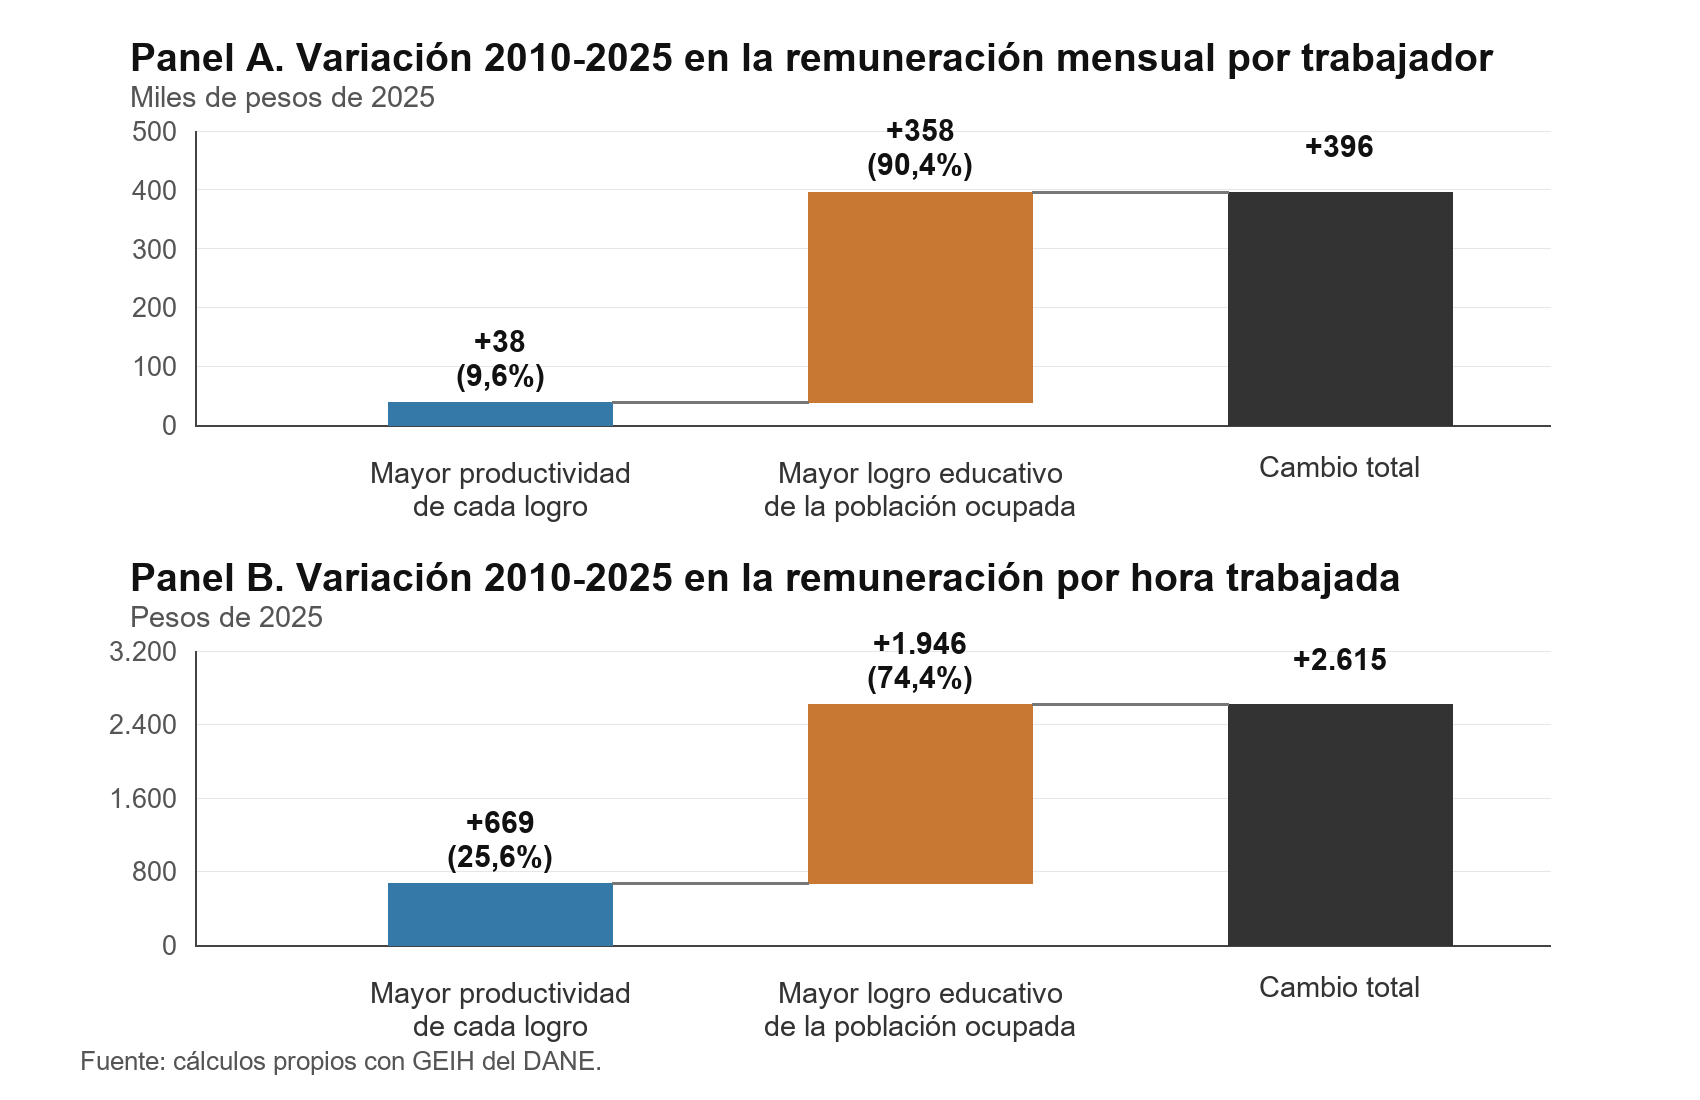
\includegraphics[width=0.98\textwidth]{Paper/figures/fig_descomposicion_remuneracion_educacion_cascada.png}
\caption*{\footnotesize %Nota: el Panel A mide la variación de la remuneración mensual por trabajador en miles de pesos de 2025. El Panel B mide la variación de la remuneración por hora trabajada en pesos de 2025 por hora. ``Mayor productividad de cada logro educativo'' mide el aporte de los cambios de remuneración dentro de cada logro educativo. ``Mayor logro educativo de la población ocupada'' mide el aporte de los cambios en el peso relativo de esos logros. La descomposición usa los ponderadores promedio de 2010 y 2025. 
Fuente: cálculos propios con GEIH del DANE.}
\end{table}


\textbf{El crecimiento de la remuneración promedio de la población ocupada estuvo impulsado principalmente por el mayor nivel educativo de los trabajadores.} El Cuadro \ref{tab:descomposicion_remuneracion_educacion} separa el aumento de la remuneración promedio en dos componentes: los cambios en la remuneración observados dentro de cada nivel educativo y los cambios en la composición educativa de la población ocupada. Entre 2010 y 2025, la remuneración mensual promedio por trabajador aumentó en 390 mil pesos mensuales de 2025. De esta variación, 140 mil pesos (35,1\%) se explican por aumentos en la remuneración de cada grupo educativo, mientras que los restantes 260 mil pesos (64,9\%) obedecen al mayor peso de los trabajadores con niveles educativos más altos dentro de la población ocupada. Un resultado similar se observa al analizar la remuneración por hora. De los 2.612 pesos de 2025 por hora que aumentó este indicador durante el período, 1.191 pesos (45,6\%) corresponden a mejoras dentro de cada nivel educativo y 1.421 pesos (54,4\%) al cambio en la composición educativa de la fuerza laboral. En conjunto, estos resultados muestran que la remuneración promedio creció más por el avance educativo de la población ocupada que por aumentos en la remuneración de cada grupo educativo. Asimismo, ayudan a explicar por qué la remuneración promedio de toda la muestra aumentó más rápido que la observada dentro de cada nivel educativo.

\textbf{Sin embargo, los aumentos sostenidos de la remuneración no podrán depender indefinidamente de que más trabajadores alcancen mayores niveles educativos.} La educación continúa siendo una de las principales vías de acceso a empleos de mejor calidad y mayores ingresos. No obstante, los resultados también muestran que el crecimiento de la remuneración entre quienes alcanzaron educación superior ha sido relativamente modesto durante los últimos quince años. En consecuencia, una estrategia orientada a elevar la productividad del país no puede limitarse a ampliar el acceso a la educación. También requiere mejorar la productividad y la capacidad de generación de ingresos de los trabajadores dentro de cada nivel educativo. Esto implica fortalecer la calidad de la formación, promover una mayor pertinencia de los programas educativos frente a las necesidades del mercado laboral y facilitar una mejor articulación entre el sistema educativo y los sectores productivos.

%\subsection{Jóvenes con educación superior: una aproximación a recién graduados}\label{subsec:recien_graduados}

%\textbf{El Cuadro \ref{tab:remuneracion_recien_graduados} y la Figura \ref{fig:remuneracion_recien_graduados_series}, incluidos en el apéndice, aproximan la remuneración de recién graduados con los ocupados de 25 a 29 años que reportan educación superior.} La GEIH no identifica si la persona acaba de graduarse ni el año de grado, por lo que esta lectura debe interpretarse como una aproximación a jóvenes con educación superior. En este grupo, los ocupados pasaron de 730 mil a 1,3 millones entre 2010 y 2025. La remuneración mensual por trabajador pasó de 2,3 a 2,4 millones de pesos mensuales de 2025, con crecimiento anual de 0,2\%. La remuneración por hora pasó de 11,7 a 12,7 miles de pesos de 2025, con crecimiento anual de 0,5\%. El resultado matiza la lectura del promedio del grupo de educación superior: la entrada al mercado laboral de los más jóvenes se expandió, pero no estuvo acompañada por un aumento fuerte de la remuneración mensual promedio.

%\textbf{La Figura \ref{fig:kernel_remuneracion_universitaria_25_29}, incluida en el apéndice, muestra la distribución de la remuneración de este mismo grupo en 2010 y 2025.} La mediana mensual pasó de 1,7 a 1,8 millones de pesos mensuales de 2025. Por hora, la mediana pasó de 8,8 a 9,6 miles de pesos de 2025. La relación entre el percentil 90 y el percentil 10 bajó tanto en la remuneración mensual como en la remuneración por hora, lo que sugiere que el aumento promedio no estuvo acompañado por una mayor dispersión dentro de este grupo.

%\textbf{El apéndice reúne los cuadros y figuras que respaldan esta lectura.} Allí se encuentran la comparación visual de la remuneración entre 2010 y 2025, las distribuciones de remuneración total y por logro educativo, las tasas laborales, la descomposición abierta por logro, la composición por sexo y formalidad, y los ejercicios sobre formalidad, edad, cohortes y recién graduados. Estos materiales permiten revisar la muestra, la distribución y la heterogeneidad detrás de los promedios usados en el cuerpo del informe.

%\section{Formalidad y remuneración por logro educativo}\label{sec:formalidad_educacion}

%\textbf{La formalidad modifica la remuneración dentro de cada logro educativo.} El Cuadro \ref{tab:remuneracion_educacion_formalidad}, incluido en el apéndice, separa a los ocupados formales e informales en los tres logros educativos comparables. En 2025, la remuneración mensual de los trabajadores formales fue de 1,7 millones de pesos en primaria o menos, 1,8 millones en secundaria o media y 3,7 millones en educación superior. Entre los informales, esos valores fueron 890 mil pesos, 1,1 millones y 1,5 millones.

%\textbf{La diferencia entre formales e informales aparece tanto por trabajador como por hora trabajada.} En 2025, la remuneración por hora de los trabajadores formales fue de 8,1 miles de pesos en primaria o menos, 8,7 miles en secundaria o media y 19,2 miles en educación superior. Entre los informales, la remuneración por hora fue de 4,9 miles de pesos, 5,8 miles y 8,7 miles. La comparación sugiere que la remuneración no depende solo del logro educativo: dentro de cada logro, la formalidad también está asociada con remuneraciones más altas.

% Bloque desactivado: material de edad y cohortes movido al apéndice.
\iffalse
\section{Remuneración por edad, cohorte y logro educativo}\label{sec:cohortes_edad}

\textbf{La comparación por grupos de edad muestra que el crecimiento de la remuneración no fue uniforme dentro de cada logro educativo.} El Cuadro \ref{tab:remuneracion_educacion_cohorte} compara la remuneración de cada grupo de edad en 2010 y 2025, para los tres logros educativos comparables. En primaria o menos, la remuneración mensual creció en todos los grupos, con aumentos anuales entre 0,5\% para 55 años o más y 1,8\% para 15 a 24 años. En secundaria o media ocurre algo parecido hasta los 54 años, pero el grupo de 55 años o más cae 0,9\% anual.

\begin{table}[H]
\centering
\caption{Remuneración laboral por logro educativo y grupo de edad, 2010 y 2025}
\label{tab:remuneracion_educacion_cohorte}
\scriptsize
\begin{tabular}{@{}p{3.6cm}p{1.6cm}rrr@{}}
\toprule
\multicolumn{5}{@{}l}{\textbf{Panel A. Remuneración mensual por trabajador (millones de pesos mensuales de 2025)}} \\
Logro educativo & Edad & 2010 & 2025 & Crec. anual \\
\midrule
Primaria o menos & 15--24 & 0,7 & 0,9 & 1,8\% \\
Primaria o menos & 25--34 & 0,9 & 1,0 & 0,9\% \\
Primaria o menos & 35--44 & 0,9 & 1,1 & 0,9\% \\
Primaria o menos & 45--54 & 0,9 & 1,1 & 1,2\% \\
Primaria o menos & 55 o más & 0,8 & 0,9 & 0,5\% \\
\addlinespace[0.3em]
Secundaria & 15--24 & 0,9 & 1,1 & 1,8\% \\
Secundaria & 25--34 & 1,2 & 1,4 & 1,0\% \\
Secundaria & 35--44 & 1,3 & 1,4 & 0,5\% \\
Secundaria & 45--54 & 1,4 & 1,4 & 0,2\% \\
Secundaria & 55 o más & 1,5 & 1,3 & -0,9\% \\
\addlinespace[0.3em]
Universitaria o superior & 15--24 & 1,3 & 1,6 & 1,2\% \\
Universitaria o superior & 25--34 & 2,6 & 2,7 & 0,2\% \\
Universitaria o superior & 35--44 & 3,5 & 3,7 & 0,3\% \\
Universitaria o superior & 45--54 & 4,4 & 4,0 & -0,6\% \\
Universitaria o superior & 55 o más & 4,8 & 4,1 & -1,1\% \\
\addlinespace[0.7em]
\multicolumn{5}{@{}l}{\textbf{Panel B. Remuneración por hora trabajada (miles de pesos de 2025 por hora)}} \\
Logro educativo & Edad & 2010 & 2025 & Crec. anual \\
\midrule
Primaria o menos & 15--24 & 3,4 & 4,8 & 2,3\% \\
Primaria o menos & 25--34 & 4,3 & 5,4 & 1,5\% \\
Primaria o menos & 35--44 & 4,5 & 5,6 & 1,5\% \\
Primaria o menos & 45--54 & 4,4 & 5,8 & 1,8\% \\
Primaria o menos & 55 o más & 4,4 & 5,1 & 1,0\% \\
\addlinespace[0.3em]
Secundaria & 15--24 & 4,4 & 6,1 & 2,2\% \\
Secundaria & 25--34 & 5,4 & 6,9 & 1,7\% \\
Secundaria & 35--44 & 6,1 & 7,2 & 1,1\% \\
Secundaria & 45--54 & 6,5 & 7,2 & 0,7\% \\
Secundaria & 55 o más & 7,8 & 7,3 & -0,5\% \\
\addlinespace[0.3em]
Universitaria o superior & 15--24 & 7,4 & 9,1 & 1,4\% \\
Universitaria o superior & 25--34 & 13,1 & 14,1 & 0,5\% \\
Universitaria o superior & 35--44 & 17,8 & 19,0 & 0,5\% \\
Universitaria o superior & 45--54 & 23,0 & 21,3 & -0,5\% \\
Universitaria o superior & 55 o más & 27,2 & 23,4 & -1,0\% \\
\bottomrule
\end{tabular}
\caption*{\footnotesize Nota: el crecimiento es anualizado para 2010--2025. Los grupos de edad comparan personas del mismo rango etario observadas en cada año. No siguen una misma cohorte de nacimiento a lo largo del tiempo. Fuente: cálculos propios con GEIH del DANE.}
\end{table}


\textbf{En el grupo de educación superior, la comparación por edad matiza el promedio agregado.} Entre 2010 y 2025, la remuneración mensual de 15 a 24 años aumentó 1,2\% anual, mientras la de 25 a 44 años cambió poco y la de 45 años o más cayó. La remuneración por hora muestra el mismo patrón: aumentó para los menores de 45 años y cayó para los mayores. Esta lectura no implica que una persona con este logro educativo pierda remuneración al envejecer. Lo que muestra es que los trabajadores de la misma edad observados en 2025 no tuvieron, en promedio, la misma remuneración que los trabajadores de esa edad observados en 2010.

\textbf{La comparación por cohortes de nacimiento agrega una lectura de ciclo de vida.} El Cuadro \ref{tab:remuneracion_educacion_cohortes_nacimiento} compara tres cohortes que aparecen tanto en 2010 como en 2025: nacidos entre 1985 y 1989, 1980 y 1984, y 1975 y 1979. Para el total, la cohorte 1985--1990 pasó de 1,2 a 2,3 millones de pesos mensuales de 2025, con crecimiento anual de 4,5\%. La cohorte 1980--1985 pasó de 1,5 a 2,2 millones, con crecimiento anual de 2,6\%. La cohorte 1975--1980 pasó de 1,7 a 2,2 millones, con crecimiento anual de 1,8\%.

\begin{table}[H]
\centering
\caption{Remuneración laboral por cohorte de nacimiento y logro educativo, 2010 y 2025}
\label{tab:remuneracion_educacion_cohortes_nacimiento}
\scriptsize
\begin{tabular}{@{}p{2.0cm}p{3.5cm}rrr@{}}
\toprule
\multicolumn{5}{@{}l}{\textbf{Panel A. Remuneración mensual por trabajador (millones de pesos mensuales de 2025)}} \\
Cohorte & Logro educativo & 2010 & 2025 & Crec. anual \\
\midrule
1985--1990 & \textbf{Total} & 1,16 & 2,26 & 4,54\% \\
1985--1990 & Primaria o menos & 0,75 & 1,08 & 2,49\% \\
1985--1990 & Secundaria & 1,03 & 1,40 & 2,05\% \\
1985--1990 & Universitaria o superior & 1,63 & 3,69 & 5,61\% \\
\addlinespace[0.4em]
1980--1985 & \textbf{Total} & 1,52 & 2,22 & 2,58\% \\
1980--1985 & Primaria o menos & 0,85 & 1,06 & 1,54\% \\
1980--1985 & Secundaria & 1,15 & 1,44 & 1,51\% \\
1980--1985 & Universitaria o superior & 2,48 & 3,82 & 2,92\% \\
\addlinespace[0.4em]
1975--1980 & \textbf{Total} & 1,67 & 2,17 & 1,77\% \\
1975--1980 & Primaria o menos & 0,97 & 1,11 & 0,90\% \\
1975--1980 & Secundaria & 1,21 & 1,42 & 1,07\% \\
1975--1980 & Universitaria o superior & 3,02 & 4,11 & 2,07\% \\
\addlinespace[0.8em]
\multicolumn{5}{@{}l}{\textbf{Panel B. Remuneración por hora trabajada (miles de pesos de 2025 por hora)}} \\
Cohorte & Logro educativo & 2010 & 2025 & Crec. anual \\
\midrule
1985--1990 & \textbf{Total} & 5,7 & 11,6 & 4,87\% \\
1985--1990 & Primaria o menos & 3,6 & 5,7 & 3,02\% \\
1985--1990 & Secundaria & 4,9 & 7,0 & 2,52\% \\
1985--1990 & Universitaria o superior & 8,6 & 19,2 & 5,49\% \\
\addlinespace[0.4em]
1980--1985 & \textbf{Total} & 7,2 & 11,5 & 3,12\% \\
1980--1985 & Primaria o menos & 4,1 & 5,6 & 2,22\% \\
1980--1985 & Secundaria & 5,3 & 7,3 & 2,15\% \\
1980--1985 & Universitaria o superior & 12,4 & 19,9 & 3,19\% \\
\addlinespace[0.4em]
1975--1980 & \textbf{Total} & 8,0 & 11,3 & 2,34\% \\
1975--1980 & Primaria o menos & 4,7 & 5,8 & 1,49\% \\
1975--1980 & Secundaria & 5,6 & 7,3 & 1,73\% \\
1975--1980 & Universitaria o superior & 15,1 & 21,6 & 2,44\% \\
\bottomrule
\end{tabular}
\caption*{\footnotesize Nota: los rangos de cohorte son intervalos de cinco años. Por ejemplo, 1985--1990 incluye nacidos de 1985 a 1989. Se reportan las cohortes que aparecen tanto en 2010 como en 2025 dentro de los rangos solicitados. El crecimiento es anualizado para 2010--2025. Fuente: cálculos propios con GEIH del DANE.}
\end{table}


\textbf{La Figura \ref{fig:remuneracion_educacion_cohortes_nacimiento} resume la remuneración mensual por trabajador para las cohortes comparables.} La figura muestra que los aumentos son mayores para la cohorte más joven y que la pendiente es especialmente pronunciada en educación superior. En esa cohorte, los ocupados con educación superior pasaron de 1,6 a 3,7 millones de pesos mensuales de 2025. En las filas por logro educativo, la comparación no debe leerse como seguimiento de las mismas personas dentro de un mismo logro, porque algunas personas pueden completar más educación entre 2010 y 2025.

\begin{figure}[H]
  \centering
  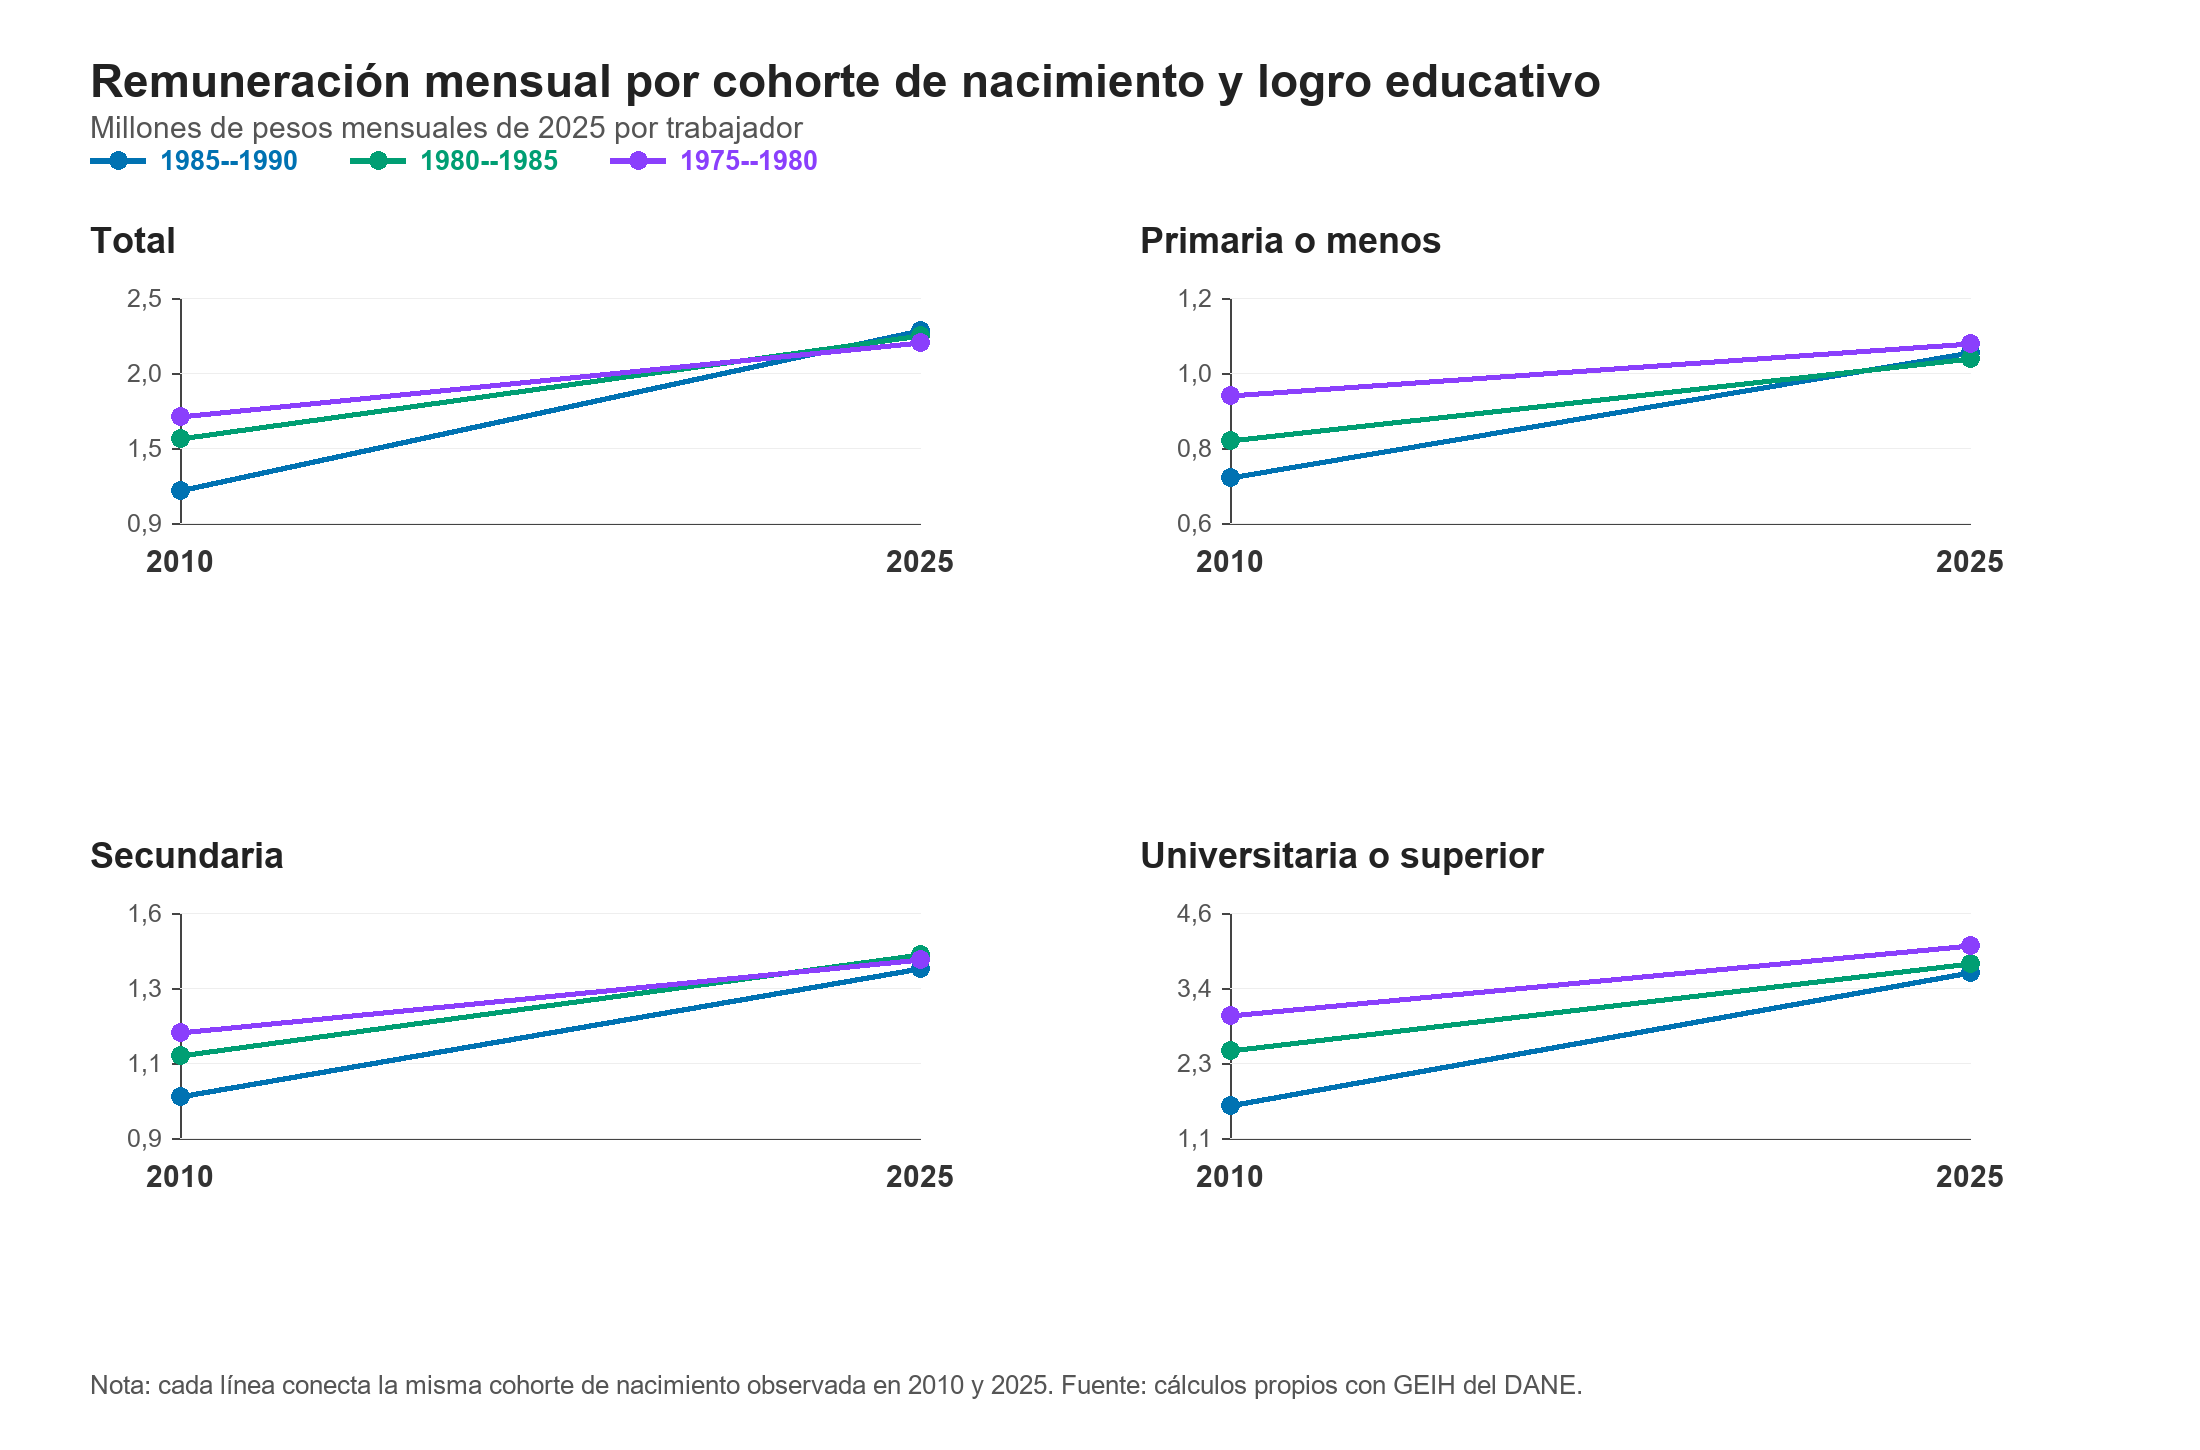
\includegraphics[width=0.98\textwidth]{Paper/figures/fig_remuneracion_educacion_cohortes_nacimiento.png}
  \caption{Remuneración mensual por cohorte de nacimiento y logro educativo, 2010 y 2025}
  \label{fig:remuneracion_educacion_cohortes_nacimiento}
  \caption*{\footnotesize Nota: millones de pesos mensuales de 2025 por trabajador. Cada línea conecta la misma cohorte de nacimiento observada en 2010 y 2025. Fuente: cálculos propios con GEIH del DANE.}
\end{figure}

\textbf{Las Figuras \ref{fig:remuneracion_cohortes_edad} y \ref{fig:remuneracion_cohortes_edad_hora} cambian el eje de comparación: en vez de poner los años en el eje horizontal, ordenan la remuneración por tramos decenales de edad.} Las figuras amplían la lectura del Cuadro \ref{tab:remuneracion_educacion_cohortes_nacimiento}: incluyen cohortes decenales cuando aparecen al menos en dos de los años disponibles. El tramo de edad se define con la edad promedio observada de cada cohorte en cada año. Usan 2010, 2015, 2021 y 2025 para mostrar cómo cambia la remuneración promedio de las cohortes a medida que avanzan en edad. La base procesada del informe no contiene 2020, por lo que 2021 se usa como primer punto disponible después de la pandemia. La lectura visual muestra trayectorias crecientes en la mayoría de cohortes, con aumentos más visibles en las cohortes jóvenes.

\begin{figure}[H]
  \centering
  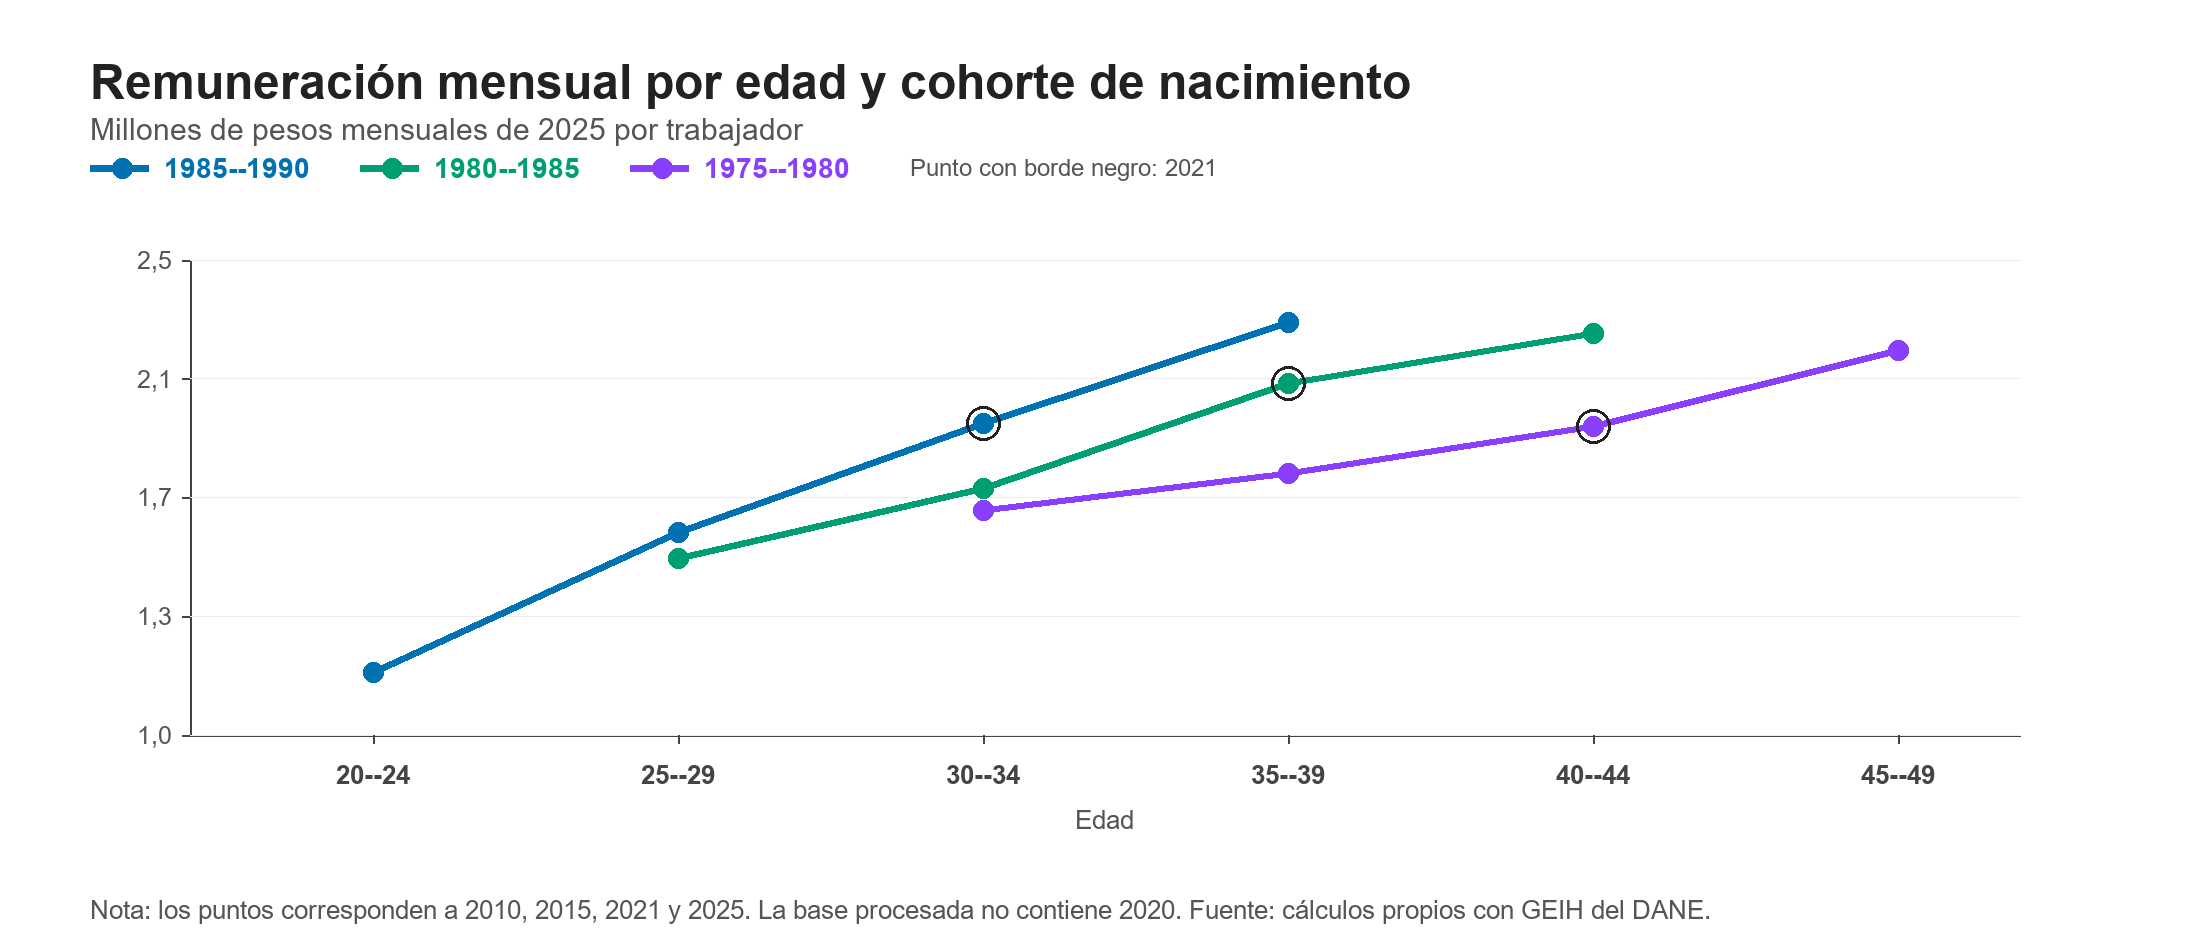
\includegraphics[width=0.98\textwidth]{Paper/figures/fig_remuneracion_cohortes_edad_trabajador.png}
  \caption{Remuneración mensual por edad y cohorte de nacimiento}
  \label{fig:remuneracion_cohortes_edad}
  \caption*{\footnotesize Nota: millones de pesos mensuales de 2025 por trabajador. Cada línea corresponde a una cohorte decenal con al menos dos años observados entre 2010, 2015, 2021 y 2025. El punto con borde abierto corresponde a 2021. La base procesada no contiene 2020. Fuente: cálculos propios con GEIH del DANE.}
\end{figure}

\begin{figure}[H]
  \centering
  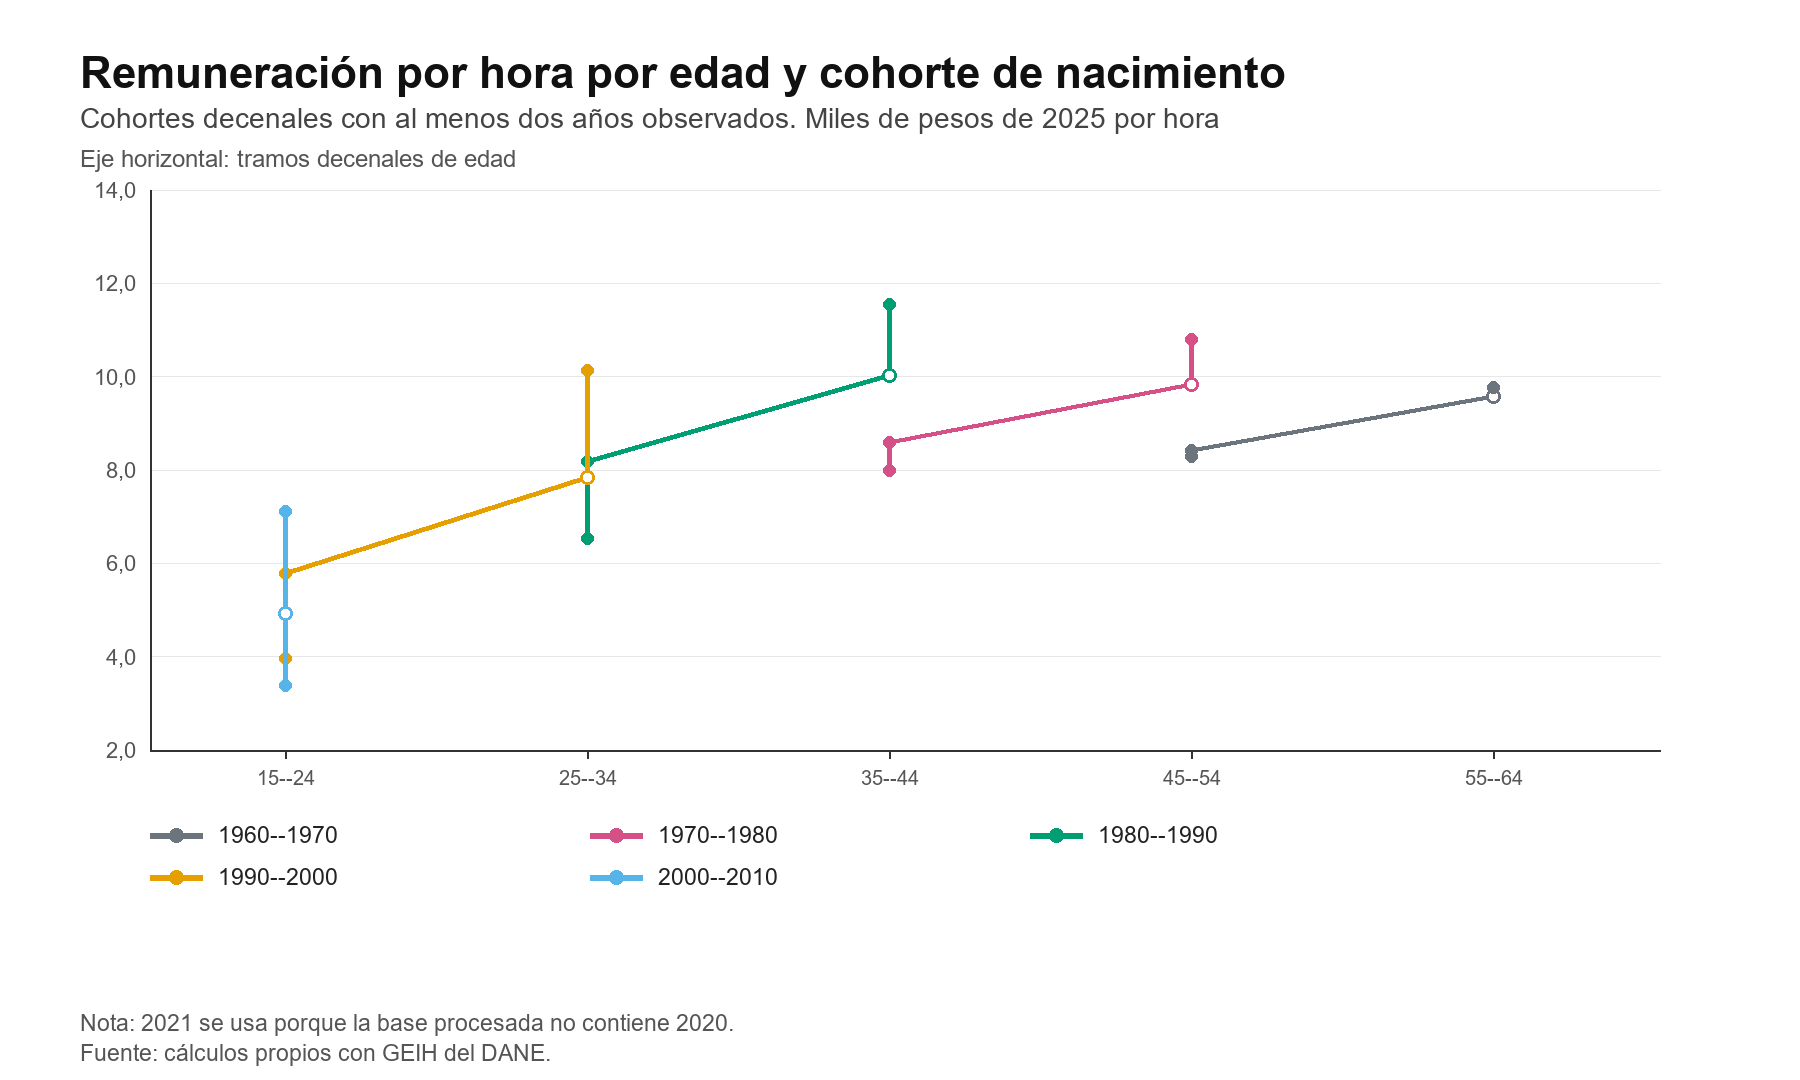
\includegraphics[width=0.98\textwidth]{Paper/figures/fig_remuneracion_cohortes_edad_hora.png}
  \caption{Remuneración por hora por edad y cohorte de nacimiento}
  \label{fig:remuneracion_cohortes_edad_hora}
  \caption*{\footnotesize Nota: miles de pesos de 2025 por hora trabajada. Cada línea corresponde a una cohorte decenal con al menos dos años observados entre 2010, 2015, 2021 y 2025. El punto con borde abierto corresponde a 2021. La base procesada no contiene 2020. Fuente: cálculos propios con GEIH del DANE.}
\end{figure}

\textbf{Las Figuras \ref{fig:remuneracion_cohortes_edad_educacion_trabajador_primaria}, \ref{fig:remuneracion_cohortes_edad_educacion_trabajador_secundaria} y \ref{fig:remuneracion_cohortes_edad_educacion_trabajador_superior} repiten la lectura por cohorte dentro de cada logro educativo para la remuneración mensual por trabajador.} Las Figuras \ref{fig:remuneracion_cohortes_edad_educacion_hora_primaria}, \ref{fig:remuneracion_cohortes_edad_educacion_hora_secundaria} y \ref{fig:remuneracion_cohortes_edad_educacion_hora_superior} hacen lo mismo para la remuneración por hora. La comparación muestra trayectorias distintas por logro educativo. En primaria o menos y secundaria o media, la remuneración se mueve en un rango más acotado. En educación superior, las cohortes jóvenes muestran aumentos más marcados. Esta lectura debe ser descriptiva, porque las personas pueden cambiar de logro educativo a lo largo del ciclo de vida.

\begin{figure}[H]
  \centering
  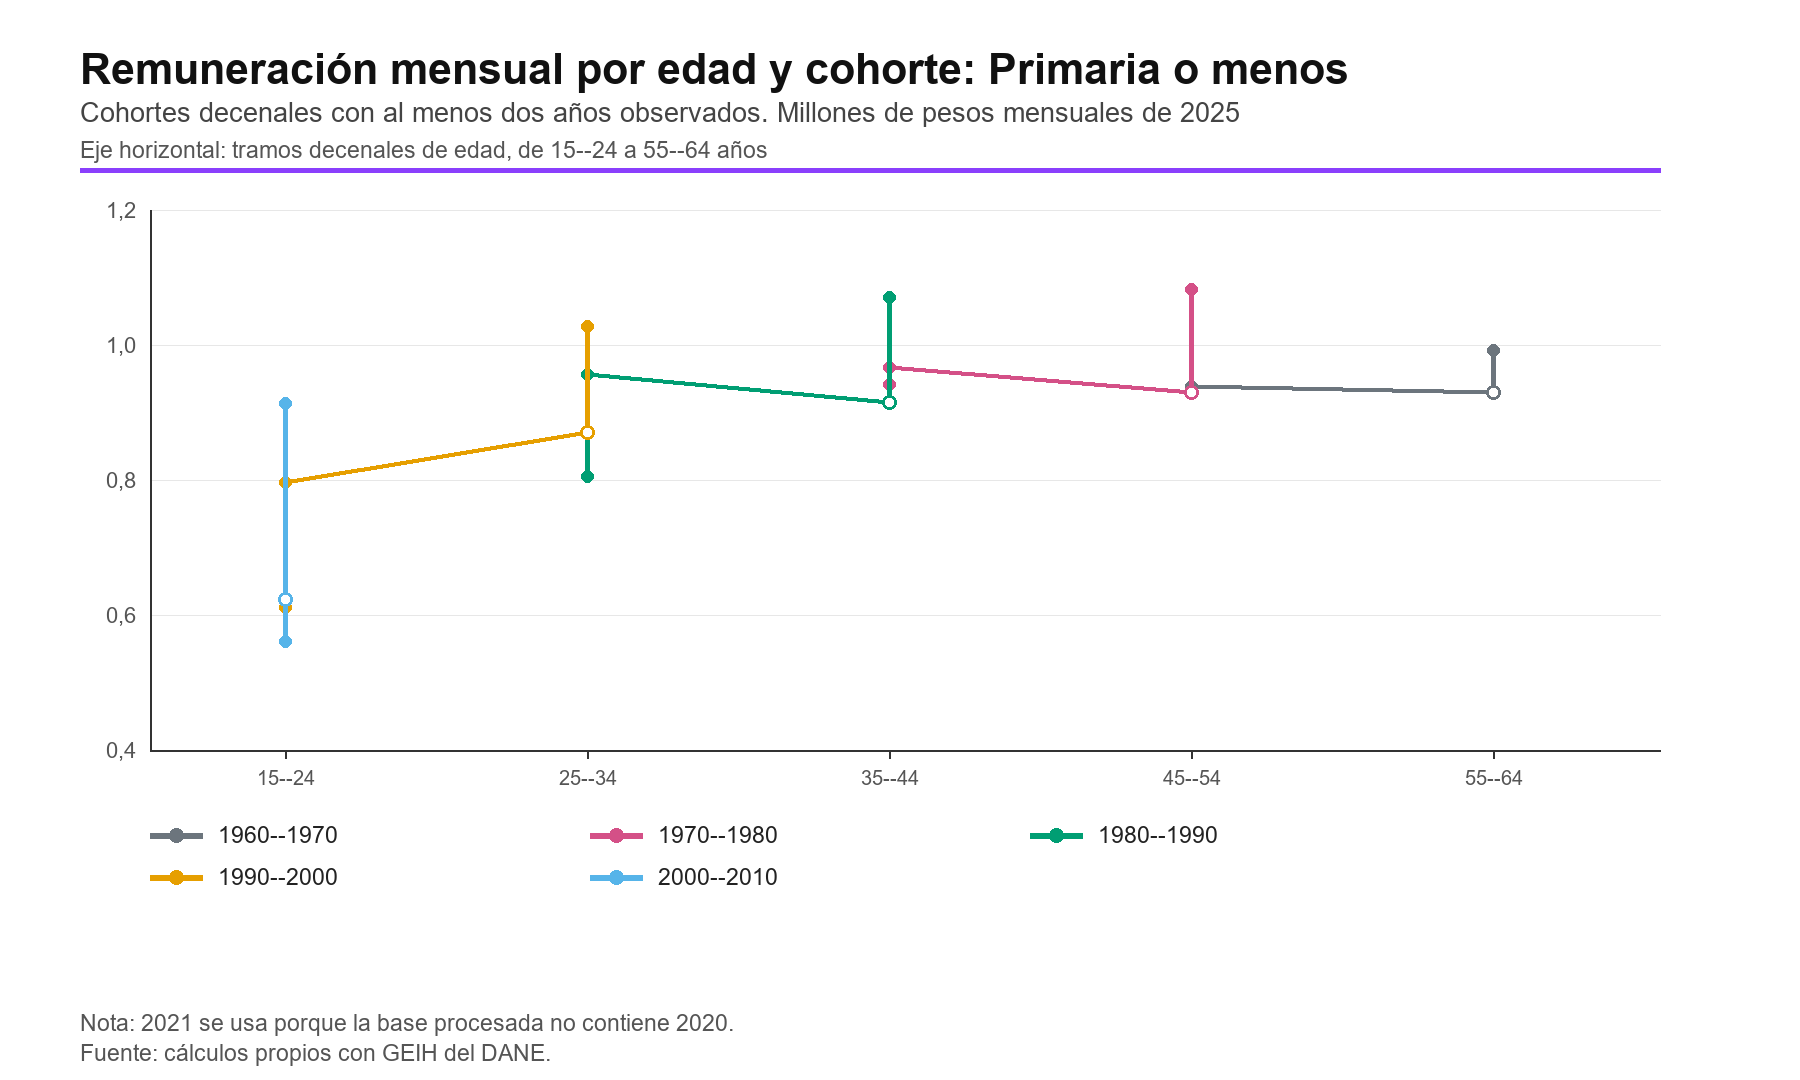
\includegraphics[width=0.98\textwidth]{Paper/figures/fig_remuneracion_cohortes_edad_educacion_trabajador_primaria.png}
  \caption{Remuneración mensual por edad y cohorte de nacimiento, primaria o menos}
  \label{fig:remuneracion_cohortes_edad_educacion_trabajador_primaria}
  \caption*{\footnotesize Nota: millones de pesos mensuales de 2025 por trabajador. Cada línea corresponde a una cohorte decenal con al menos dos años observados entre 2010, 2015, 2021 y 2025. El eje va de 15--24 a 55--64 años. El punto con borde abierto corresponde a 2021. La base procesada no contiene 2020. Fuente: cálculos propios con GEIH del DANE.}
\end{figure}

\begin{figure}[H]
  \centering
  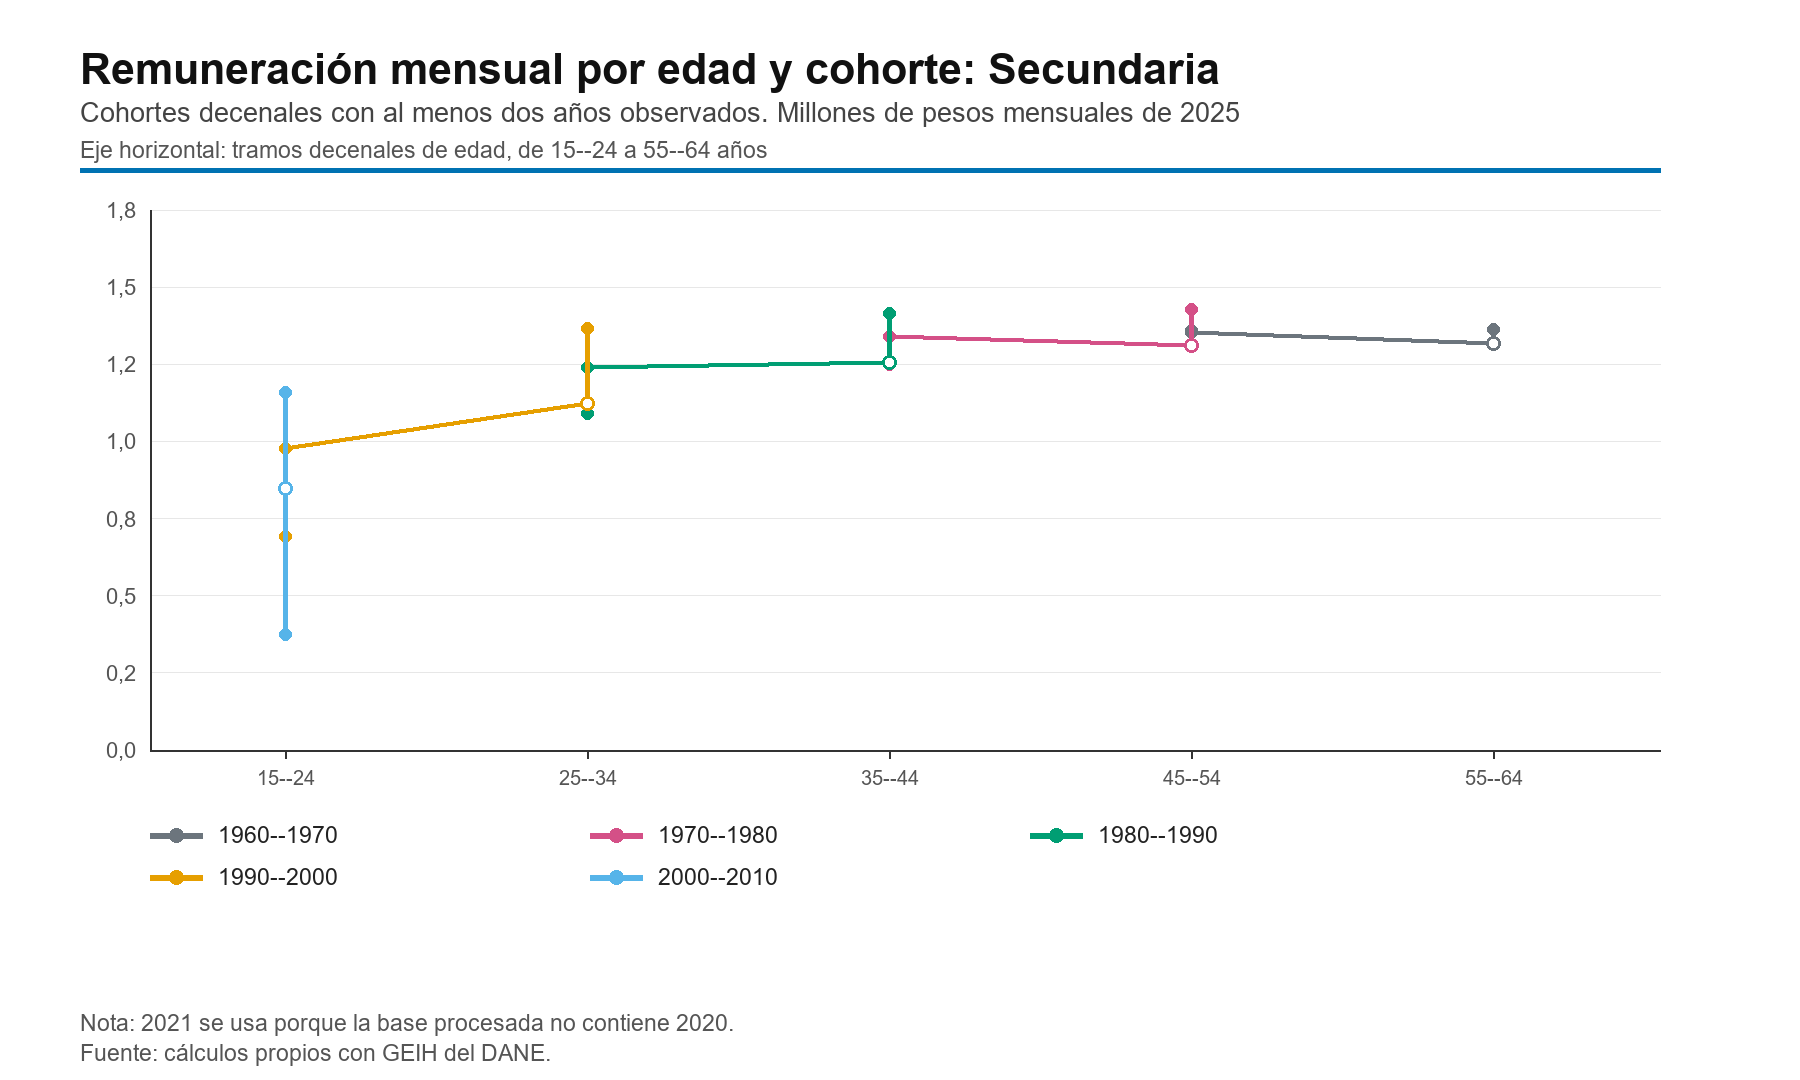
\includegraphics[width=0.98\textwidth]{Paper/figures/fig_remuneracion_cohortes_edad_educacion_trabajador_secundaria.png}
  \caption{Remuneración mensual por edad y cohorte de nacimiento, secundaria o media}
  \label{fig:remuneracion_cohortes_edad_educacion_trabajador_secundaria}
  \caption*{\footnotesize Nota: millones de pesos mensuales de 2025 por trabajador. Cada línea corresponde a una cohorte decenal con al menos dos años observados entre 2010, 2015, 2021 y 2025. El eje va de 15--24 a 55--64 años. El punto con borde abierto corresponde a 2021. La base procesada no contiene 2020. Fuente: cálculos propios con GEIH del DANE.}
\end{figure}

\begin{figure}[H]
  \centering
  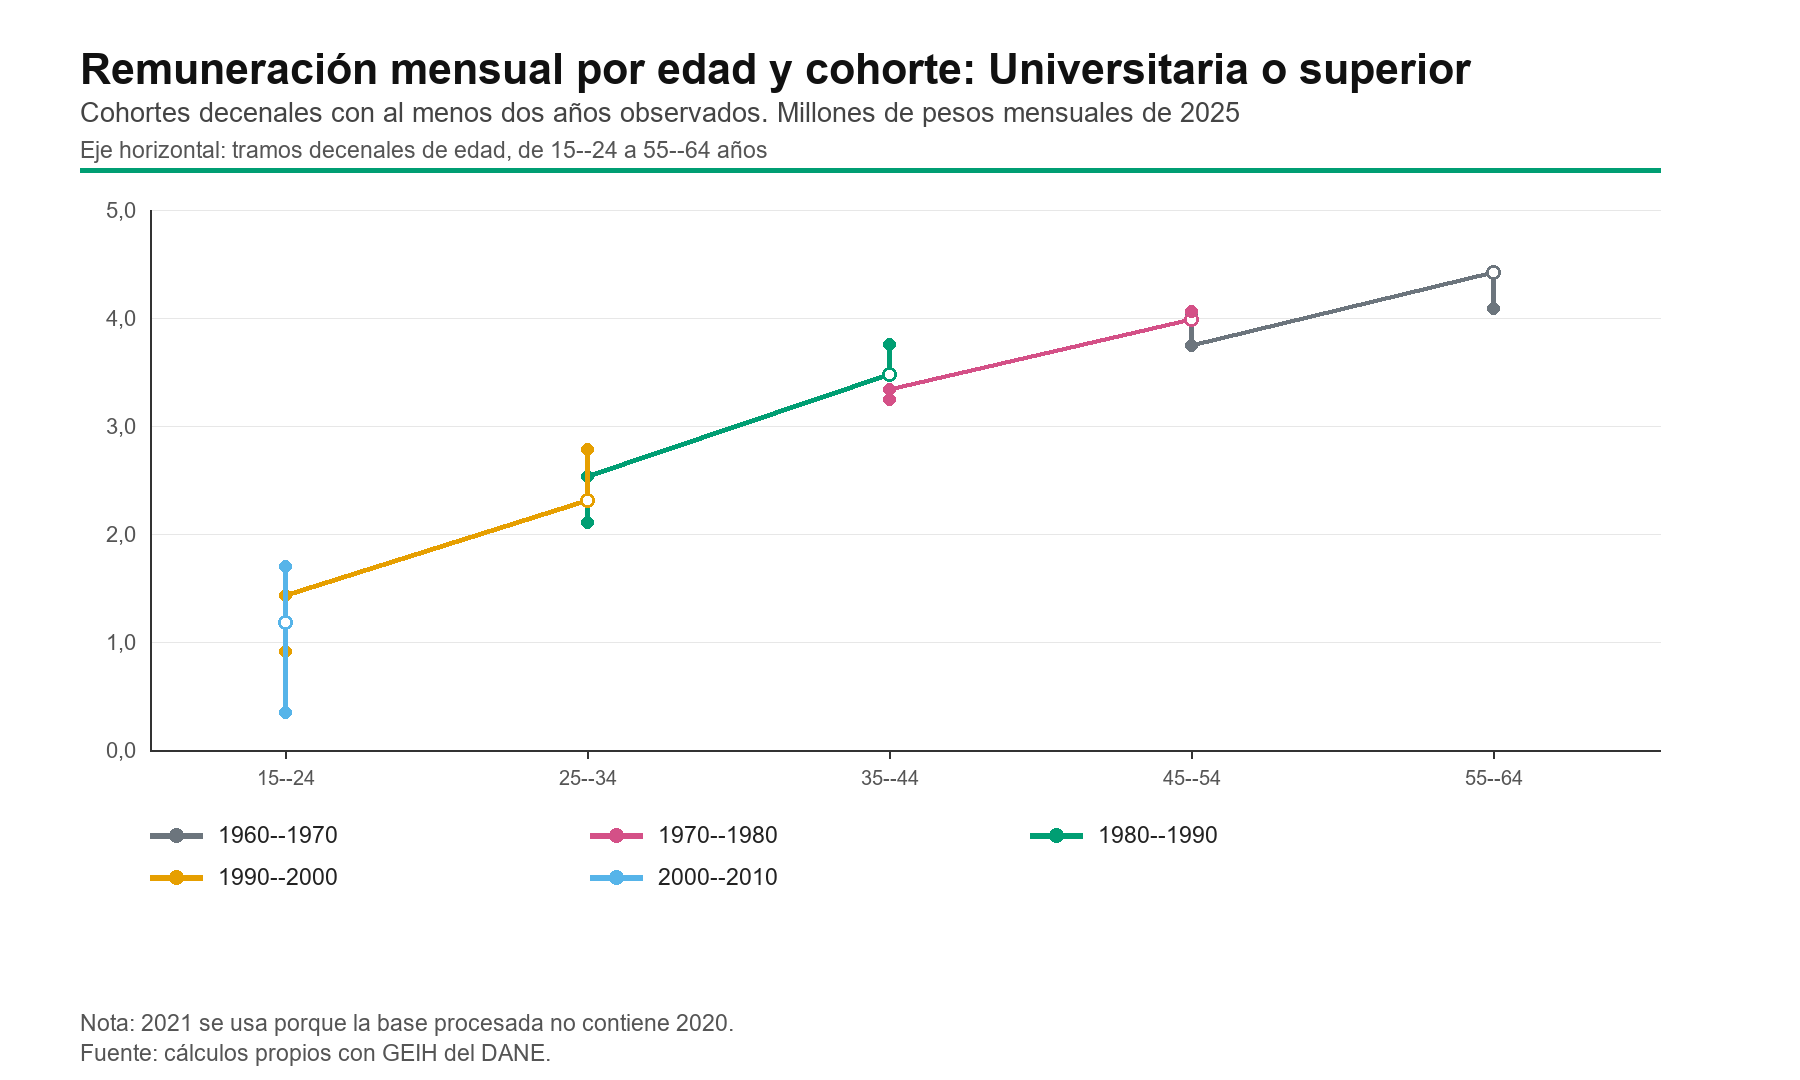
\includegraphics[width=0.98\textwidth]{Paper/figures/fig_remuneracion_cohortes_edad_educacion_trabajador_superior.png}
  \caption{Remuneración mensual por edad y cohorte de nacimiento, superior o universitaria}
  \label{fig:remuneracion_cohortes_edad_educacion_trabajador_superior}
  \caption*{\footnotesize Nota: millones de pesos mensuales de 2025 por trabajador. Cada línea corresponde a una cohorte decenal con al menos dos años observados entre 2010, 2015, 2021 y 2025. El eje va de 15--24 a 55--64 años. El punto con borde abierto corresponde a 2021. La base procesada no contiene 2020. Fuente: cálculos propios con GEIH del DANE.}
\end{figure}

\begin{figure}[H]
  \centering
  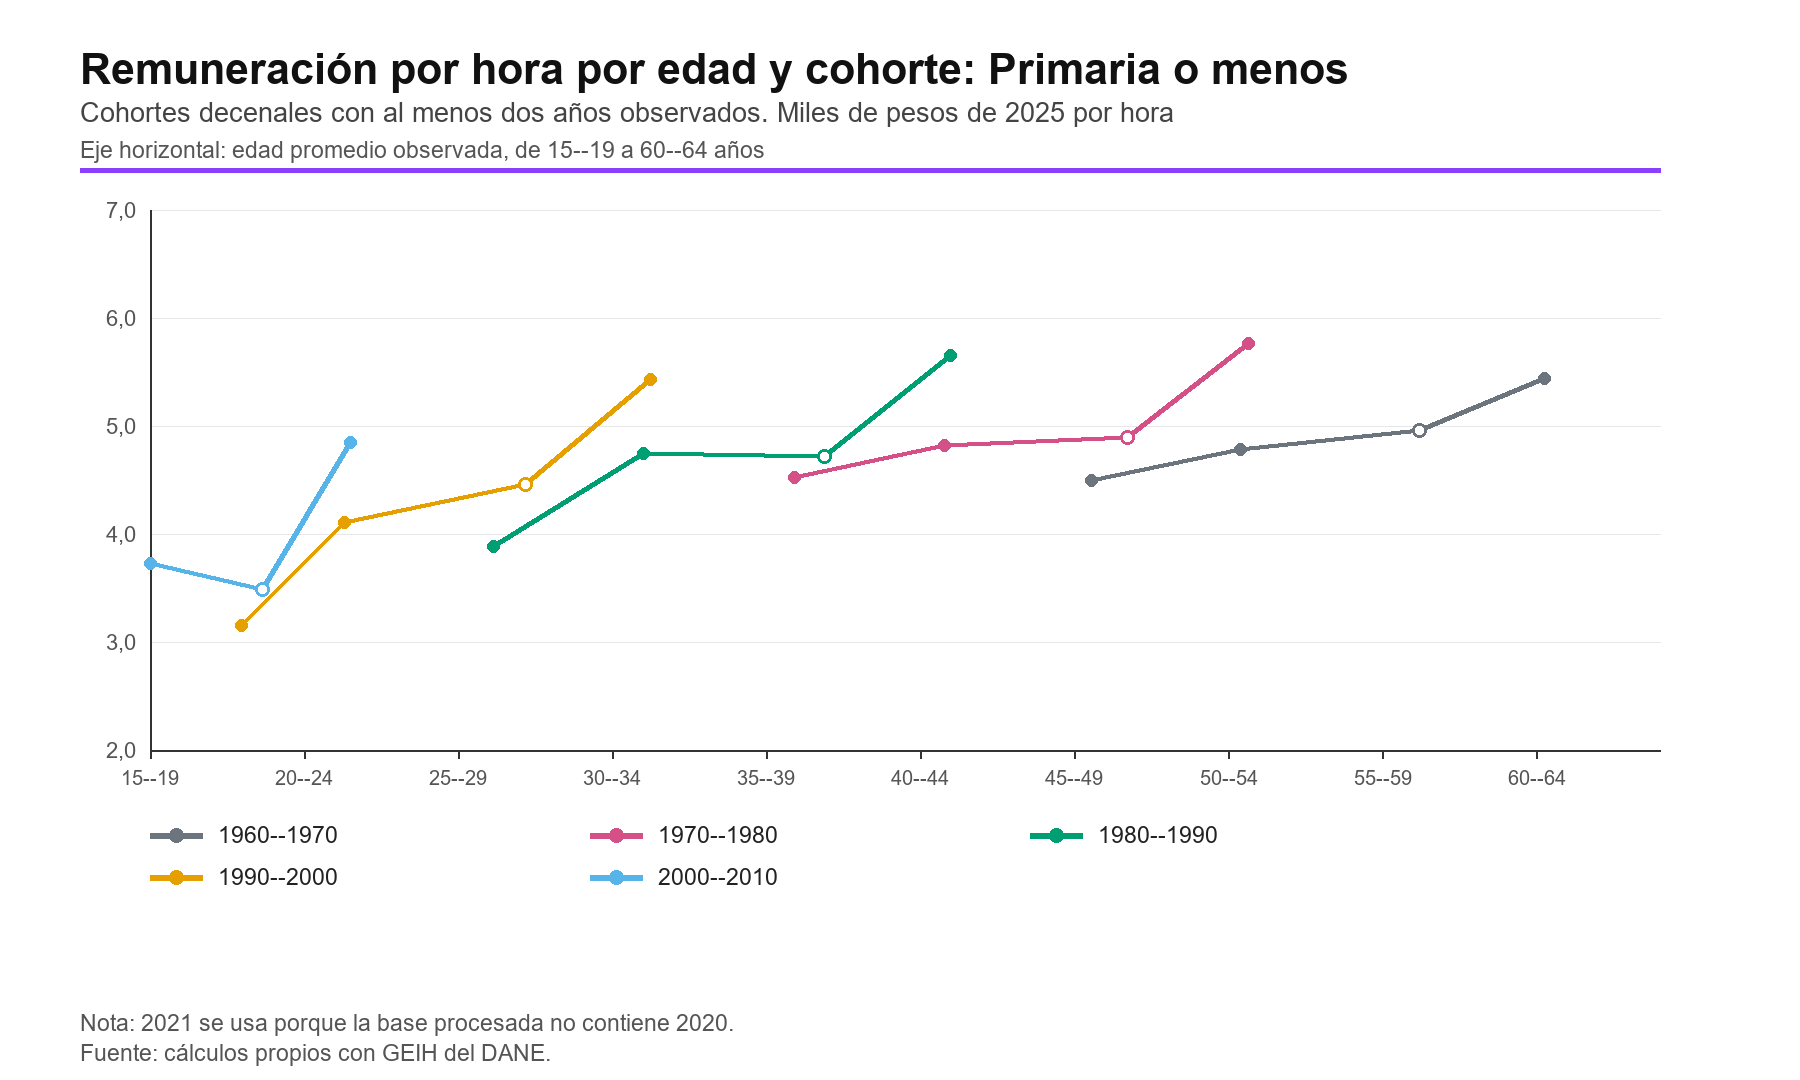
\includegraphics[width=0.98\textwidth]{Paper/figures/fig_remuneracion_cohortes_edad_educacion_hora_primaria.png}
  \caption{Remuneración por hora por edad y cohorte de nacimiento, primaria o menos}
  \label{fig:remuneracion_cohortes_edad_educacion_hora_primaria}
  \caption*{\footnotesize Nota: miles de pesos de 2025 por hora trabajada. Cada línea corresponde a una cohorte decenal con al menos dos años observados entre 2010, 2015, 2021 y 2025. El eje va de 15--24 a 55--64 años. El punto con borde abierto corresponde a 2021. La base procesada no contiene 2020. Fuente: cálculos propios con GEIH del DANE.}
\end{figure}

\begin{figure}[H]
  \centering
  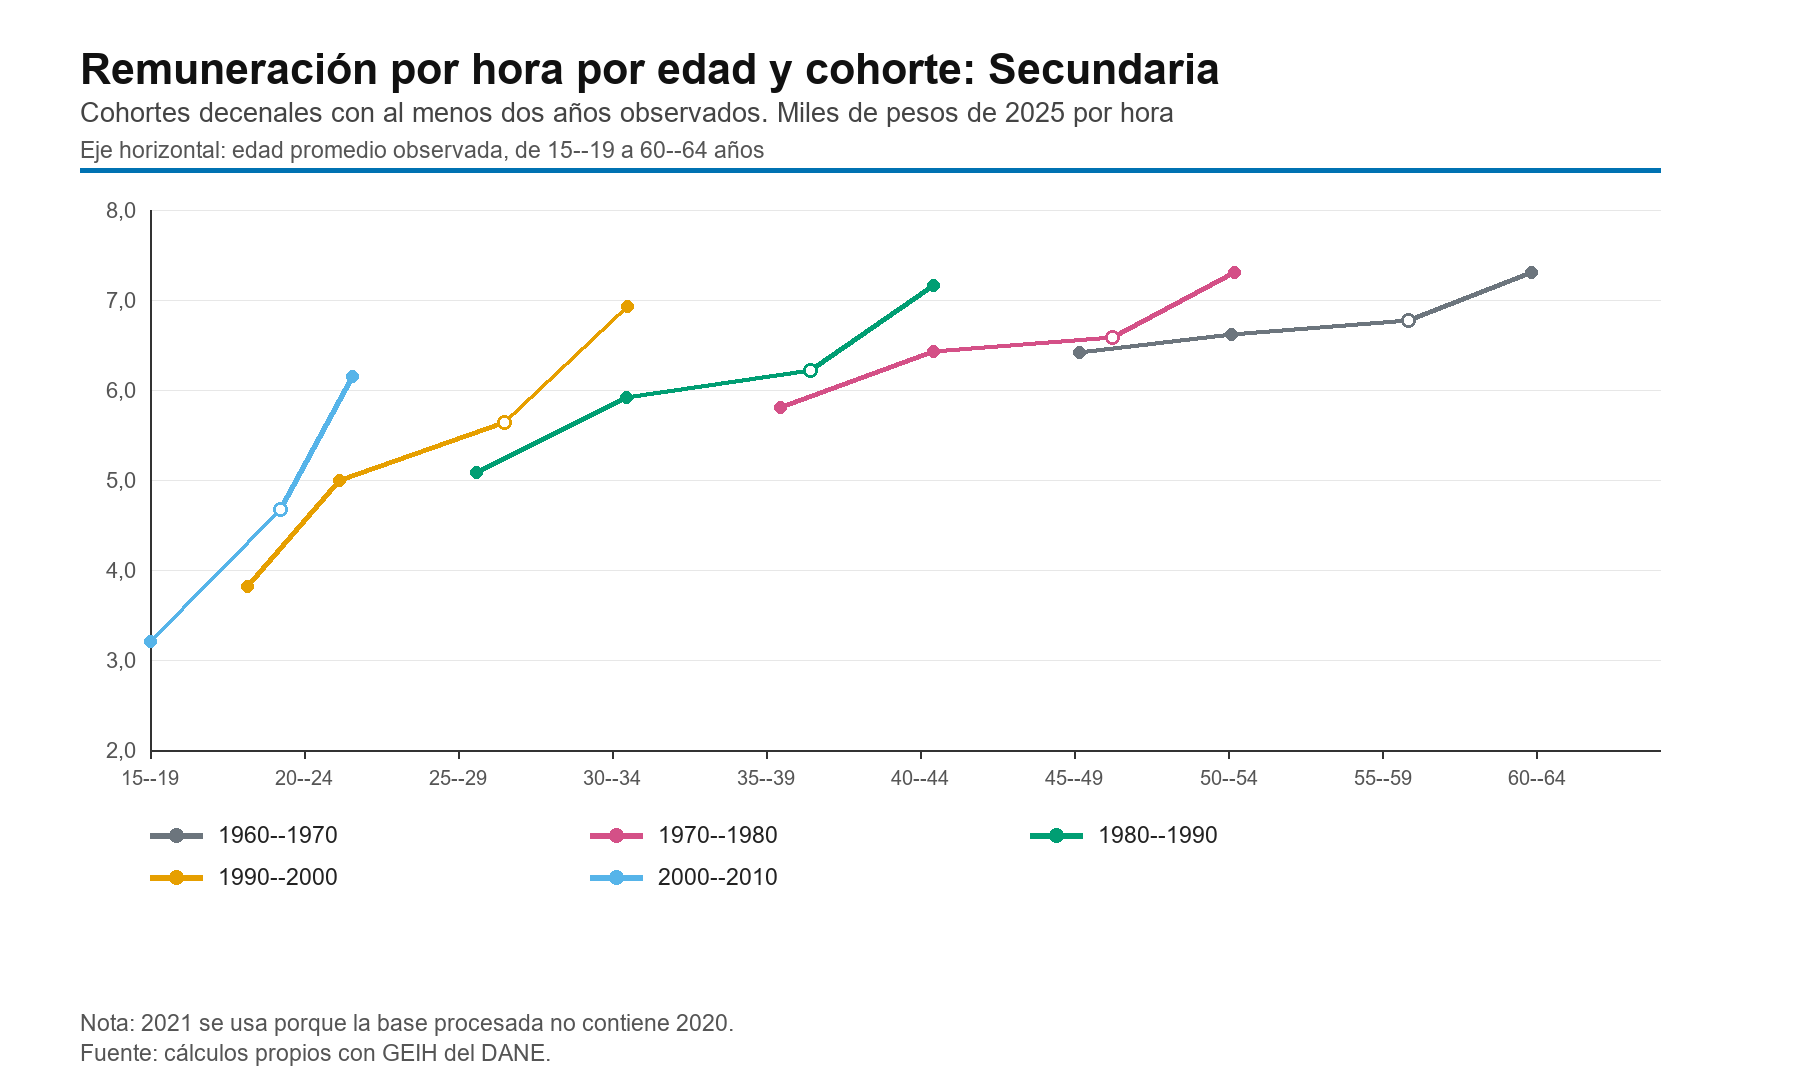
\includegraphics[width=0.98\textwidth]{Paper/figures/fig_remuneracion_cohortes_edad_educacion_hora_secundaria.png}
  \caption{Remuneración por hora por edad y cohorte de nacimiento, secundaria o media}
  \label{fig:remuneracion_cohortes_edad_educacion_hora_secundaria}
  \caption*{\footnotesize Nota: miles de pesos de 2025 por hora trabajada. Cada línea corresponde a una cohorte decenal con al menos dos años observados entre 2010, 2015, 2021 y 2025. El eje va de 15--24 a 55--64 años. El punto con borde abierto corresponde a 2021. La base procesada no contiene 2020. Fuente: cálculos propios con GEIH del DANE.}
\end{figure}

\begin{figure}[H]
  \centering
  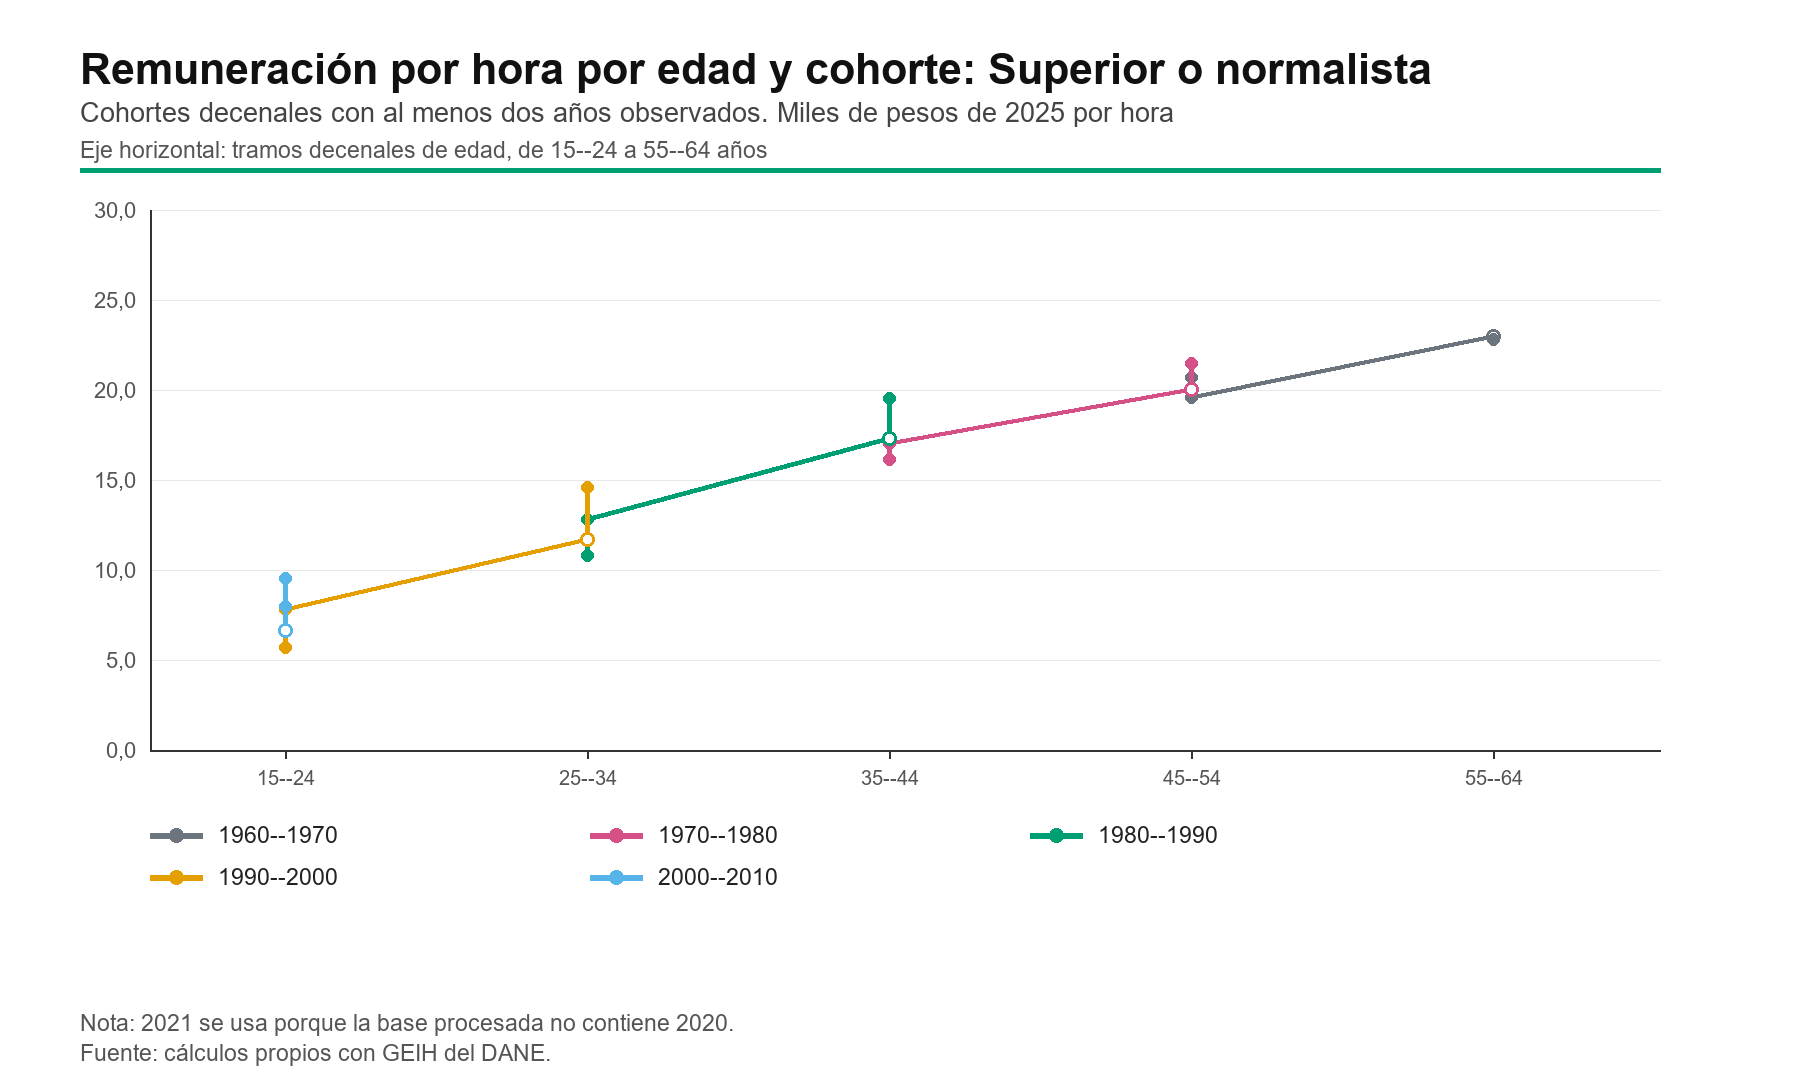
\includegraphics[width=0.98\textwidth]{Paper/figures/fig_remuneracion_cohortes_edad_educacion_hora_superior.png}
  \caption{Remuneración por hora por edad y cohorte de nacimiento, superior o universitaria}
  \label{fig:remuneracion_cohortes_edad_educacion_hora_superior}
  \caption*{\footnotesize Nota: miles de pesos de 2025 por hora trabajada. Cada línea corresponde a una cohorte decenal con al menos dos años observados entre 2010, 2015, 2021 y 2025. El eje va de 15--24 a 55--64 años. El punto con borde abierto corresponde a 2021. La base procesada no contiene 2020. Fuente: cálculos propios con GEIH del DANE.}
\end{figure}
\fi

\section{Dinámicas de corto plazo}\label{sec:categorias_detalladas}

\textbf{Desde 2021, la clasificación educativa permite distinguir con más detalle el logro educativo reportado por los ocupados.} Esta apertura complementa la lectura de largo plazo de la sección anterior. En particular, desde 2021 se puede medir la remuneración para quienes alcanzan media académica, media técnica, técnica profesional, tecnológica, pregrado universitario, especialización, maestría y doctorado. %La correspondencia entre estas categorías y el sistema educativo se presenta en el Cuadro \ref{tab:mapeo_logros_educativos}.

\textbf{El Cuadro \ref{tab:ocupacion_educacion_detallada} muestra la composición reciente del empleo por logro educativo.} En 2025, media académica fue la categoría más grande, con 7,5 millones de ocupados y 31,6\% del empleo. Le siguieron básica primaria, con 4,4 millones y 18,3\%, y universitaria, con 3,6 millones y 15,1\%. Entre 2021 y 2025, básica primaria perdió 2,0 p.p. y media académica ganó 1,1 p.p.

%\textbf{La diferencia entre ocupación total y submuestra de remuneración es importante para leer los cuadros siguientes.} En 2021, los ocupados con logro educativo válido sumaban 20,4 millones, pero los ocupados con ingreso y horas válidos sumaban 17,6 millones. En 2025, esos valores fueron 23,8 y 23,0 millones. Por eso, el Cuadro \ref{tab:ocupacion_educacion_detallada} describe la composición del empleo, mientras el Cuadro \ref{tab:remuneracion_educacion_detallada} usa la submuestra con información suficiente para calcular remuneraciones.

\begin{table}[H]
\centering
\caption{Ocupación por logro educativo detallado, 2021 y 2025}
\label{tab:ocupacion_educacion_detallada}
\scriptsize
\begin{tabular}{@{}p{4.2cm}p{8.5cm}@{}}
\toprule
Logro educativo & Ocupación y participación \\
\midrule
Preescolar o ninguno & 2021: 0,6 mill. (3,6\%)\newline 2025: 0,7 mill. (2,9\%)\newline Dif.: -0,7 p.p. \\
Básica primaria & 2021: 3,7 mill. (20,8\%)\newline 2025: 4,2 mill. (18,1\%)\newline Dif.: -2,7 p.p. \\
Básica secundaria & 2021: 2,1 mill. (12,0\%)\newline 2025: 2,5 mill. (10,8\%)\newline Dif.: -1,2 p.p. \\
Media académica & 2021: 5,5 mill. (31,1\%)\newline 2025: 7,3 mill. (31,8\%)\newline Dif.: +0,7 p.p. \\
Media técnica & 2021: 0,4 mill. (2,4\%)\newline 2025: 0,6 mill. (2,7\%)\newline Dif.: +0,3 p.p. \\
Normalista & 2021: 0,0 mill. (0,2\%)\newline 2025: 0,0 mill. (0,1\%)\newline Dif.: -0,1 p.p. \\
Técnica profesional & 2021: 1,3 mill. (7,6\%)\newline 2025: 1,9 mill. (8,3\%)\newline Dif.: +0,7 p.p. \\
Tecnológica & 2021: 0,7 mill. (3,9\%)\newline 2025: 1,0 mill. (4,4\%)\newline Dif.: +0,6 p.p. \\
Universitaria & 2021: 2,4 mill. (13,8\%)\newline 2025: 3,5 mill. (15,1\%)\newline Dif.: +1,3 p.p. \\
Especialización & 2021: 0,5 mill. (3,0\%)\newline 2025: 0,8 mill. (3,5\%)\newline Dif.: +0,6 p.p. \\
Maestría & 2021: 0,3 mill. (1,5\%)\newline 2025: 0,4 mill. (2,0\%)\newline Dif.: +0,4 p.p. \\
Doctorado & 2021: 0,0 mill. (0,2\%)\newline 2025: 0,1 mill. (0,3\%)\newline Dif.: +0,1 p.p. \\
\midrule
\textbf{Total} & 2021: 17,6 mill. (100,0\%)\newline 2025: 23,0 mill. (100,0\%)\newline Dif.: 0,0 p.p. \\
\bottomrule
\end{tabular}
\caption*{\footnotesize Nota: ocupados en millones de personas. Entre paréntesis se reporta la participación en el empleo. Dif. corresponde al cambio en participación, en puntos porcentuales. Los 0,0 pueden corresponder a menos de 50 mil ocupados. Fuente: cálculos propios con GEIH del DANE.}
\end{table}


\begin{table}[H]
\centering
\caption{Ocupación por logro educativo detallado, 2021 y 2025}
\label{tab:ocupacion_educacion_detallada}
\footnotesize
\begin{tabular}{@{}p{4.3cm}rrrrr@{}}
\toprule
Logro educativo & Ocupados 2021 & Ocupados 2025 & Part. 2021 & Part. 2025 & Dif. (p.p.) \\
\midrule
Preescolar o ninguno & 0,63 & 0,67 & 3,6\% & 2,9\% & -0,7 \\
Básica primaria & 3,67 & 4,15 & 20,8\% & 18,1\% & -2,7 \\
Básica secundaria & 2,11 & 2,49 & 12,0\% & 10,8\% & -1,2 \\
Media académica & 5,47 & 7,29 & 31,1\% & 31,8\% & 0,7 \\
Media técnica & 0,42 & 0,61 & 2,4\% & 2,7\% & 0,3 \\
Normalista & 0,03 & 0,03 & 0,2\% & 0,1\% & -0,1 \\
Técnica profesional & 1,34 & 1,91 & 7,6\% & 8,3\% & 0,7 \\
Tecnológica & 0,68 & 1,02 & 3,9\% & 4,4\% & 0,6 \\
Universitaria & 2,44 & 3,47 & 13,8\% & 15,1\% & 1,3 \\
Especialización & 0,52 & 0,81 & 3,0\% & 3,5\% & 0,6 \\
Maestría & 0,27 & 0,45 & 1,5\% & 2,0\% & 0,4 \\
Doctorado & 0,03 & 0,06 & 0,2\% & 0,3\% & 0,1 \\
\midrule
\textbf{Total} & 17,60 & 22,96 & 100,0\% & 100,0\% & 0,0 \\
\bottomrule
\end{tabular}
\caption*{\footnotesize Nota: ocupados en millones de personas. Participaciones en porcentaje. Diferencia en puntos porcentuales. Fuente: cálculos propios con GEIH del DANE.}
\end{table}

\begin{table}[H]
\centering
\caption{Remuneración mensual por trabajador por logro educativo detallado, 2021 y 2025}
\label{tab:remuneracion_educacion_detallada_trabajador}
\footnotesize
\begin{tabular}{@{}p{5.1cm}rrr@{}}
\toprule
Logro educativo & 2021 & 2025 & Crec. anual \\
\midrule
Preescolar o ninguno & 0,73 & 0,78 & 1,76\% \\
Básica primaria & 0,91 & 1,03 & 3,12\% \\
Básica secundaria & 1,00 & 1,15 & 3,66\% \\
Media académica & 1,22 & 1,39 & 3,25\% \\
Media técnica & 1,73 & 1,52 & -3,08\% \\
Normalista & 1,83 & 1,97 & 1,83\% \\
Técnica profesional & 1,60 & 1,64 & 0,60\% \\
Tecnológica & 1,89 & 2,00 & 1,52\% \\
Universitaria & 3,31 & 3,15 & -1,26\% \\
Especialización & 6,49 & 6,06 & -1,71\% \\
Maestría & 7,30 & 7,48 & 0,61\% \\
Doctorado & 9,26 & 9,97 & 1,86\% \\
\midrule
\textbf{Total} & 1,73 & 1,91 & 2,43\% \\
\bottomrule
\end{tabular}
\caption*{\footnotesize Nota: la remuneración mensual por trabajador se expresa en millones de pesos mensuales de 2025. Las filas detalladas se calibran con un factor común dentro de cada grupo comparable para que la apertura detallada quede anclada al valor del Cuadro \ref{tab:remuneracion_educacion_remuneracion}. La calibración preserva las diferencias relativas entre categorías detalladas. El crecimiento es anualizado para 2021--2025. Fuente: cálculos propios con GEIH del DANE.}
\end{table}

\begin{table}[H]
\centering
\caption{Remuneración por hora trabajada por logro educativo detallado, 2021 y 2025}
\label{tab:remuneracion_educacion_detallada}
\footnotesize
\begin{tabular}{@{}p{5.1cm}rrr@{}}
\toprule
Logro educativo & 2021 & 2025 & Crec. anual \\
\midrule
Preescolar o ninguno & 3,9 & 4,3 & 2,26\% \\
Básica primaria & 4,9 & 5,6 & 3,63\% \\
Básica secundaria & 5,1 & 6,0 & 4,13\% \\
Media académica & 6,2 & 7,2 & 3,72\% \\
Media técnica & 8,8 & 7,9 & -2,65\% \\
Normalista & 9,3 & 10,5 & 3,03\% \\
Técnica profesional & 8,1 & 8,7 & 1,79\% \\
Tecnológica & 9,6 & 10,7 & 2,72\% \\
Universitaria & 16,8 & 16,8 & -0,09\% \\
Especialización & 33,0 & 32,2 & -0,55\% \\
Maestría & 37,1 & 39,8 & 1,80\% \\
Doctorado & 47,0 & 53,1 & 3,07\% \\
\midrule
\textbf{Total} & 8,9 & 10,1 & 3,11\% \\
\bottomrule
\end{tabular}
\caption*{\footnotesize Nota: la remuneración por hora se expresa en miles de pesos de 2025 por hora trabajada. Las filas detalladas se calibran con un factor común dentro de cada grupo comparable para que la apertura detallada quede anclada al valor del Cuadro \ref{tab:remuneracion_educacion_remuneracion}. La calibración preserva las diferencias relativas entre categorías detalladas. El crecimiento es anualizado para 2021--2025. Fuente: cálculos propios con GEIH del DANE.}
\end{table}


\textbf{Las diferencias de remuneración son más amplias cuando el logro educativo se desagrega.} El Cuadro \ref{tab:remuneracion_educacion_detallada} reporta la remuneración mensual por trabajador y la remuneración por hora para cada logro educativo detallado. En 2025, la remuneración mensual promedio fue de 740 mil pesos para preescolar o ninguno y de 9,3 millones de pesos para doctorado. La remuneración por hora siguió el mismo orden: 4,3 mil pesos y 53,4 mil pesos, respectivamente. La educación universitaria se ubicó en un punto intermedio, con 3,1 millones de pesos mensuales y 16,8 mil pesos por hora. Dentro de secundaria o media, media técnica reportó una remuneración ligeramente mayor que media académica en las dos medidas.

\textbf{Entre 2021 y 2025, la remuneración de quienes tienen pregrado universitario no aumentó en términos reales.} En los logros previos a la educación superior, la remuneración aumentó tanto por trabajador como por hora. La remuneración también aumentó entre quienes reportaron formación normalista, técnica profesional, tecnológica, maestría o doctorado. En cambio, cayó para educación universitaria cuando se mide por trabajador y casi no cambió cuando se mide por hora. La remuneración de especialización cayó en ambas medidas. %Por eso, el promedio de educación superior combina credenciales con aumentos, caídas y estabilidad en la remuneración.

\textbf{Los logros educativos detallados también están asociados con resultados laborales que van más allá de la remuneración.} Además de las diferencias de remuneración, el logro educativo se relaciona con las tasas de participación, ocupación, desempleo y formalidad. El Cuadro \ref{tab:tasas-laborales-educacion-detallada-2021-2025}, incluido en el apéndice, presenta estas tasas para los logros educativos detallados. Particularmente sobresale la formalidad: en 2025, la tasa de formalidad fue 3,9\% entre quienes reportaron preescolar o ninguno, 40,5\% en media académica, 76,4\% en universitaria y 98,4\% en doctorado.

\textbf{La distribución de la remuneración para quienes tienen pregrado universitario da indicios de diversidad en la calidad de los egresados.} La Figura \ref{fig:kernel_remuneracion_credenciales_superiores} compara las distribuciones de 2021 y 2025 para educación universitaria, especialización y maestría. En educación universitaria, los paneles mensuales muestran una concentración de ocupados cerca del salario mínimo y otra alrededor de la media. Esta distribución es compatible con diferencias en la calidad de los egresados, aunque se requiere más investigación para verificar esta hipótesis.

\textbf{La mirada a la remuneración de los recién egresados de pregrado puede ayudar a dilucidar las razones para el estancamiento de la remuneración universitaria.} El Cuadro \ref{tab:remuneracion_pregrado_universitario_25_29} %y la Figura \ref{fig:kernel_pregrado_universitario_25_29} 
restringe la muestra a ocupados de 25 a 29 años que reportan pregrado universitario. En este grupo, la remuneración mensual promedio cayó de 3,1 a 2,8 millones de pesos entre 2021 y 2025, mientras la mediana se mantuvo en 2,5 millones. La remuneración por hora promedio cayó de 16,4 a 15,6 mil pesos, aunque la mediana aumentó de 11,8 a 13,0 mil pesos. La distribución también se volvió menos dispersa y aumentó la proporción de ocupados con remuneración mensual cercana al salario mínimo. 

\begin{table}[H]
\centering
\caption{Remuneración de ocupados de 25 a 29 años con pregrado universitario, 2021 y 2025}
\label{tab:remuneracion_pregrado_universitario_25_29}
\footnotesize
\begin{tabular}{@{}p{7.4cm}rr@{}}
\toprule
Indicador & 2021 & 2025 \\
\midrule
\multicolumn{3}{@{}l}{\textbf{Panel A. Remuneración mensual por trabajador}} \\
Ocupados (miles) & 347,1 & 454,7 \\
Promedio (millones de pesos de 2025) & 3,1 & 2,8 \\
Mediana (millones de pesos de 2025) & 2,5 & 2,5 \\
Desviación estándar (millones de pesos de 2025) & 3,6 & 1,9 \\
Razón P90/P10 & 4,9 & 3,6 \\
Entre 0,9 y 1,1 SMLMV & 8,8\% & 13,3\% \\
\addlinespace[0.6em]
\multicolumn{3}{@{}l}{\textbf{Panel B. Remuneración por hora trabajada}} \\
Promedio (miles de pesos de 2025) & 16,4 & 15,6 \\
Mediana (miles de pesos de 2025) & 11,8 & 13,0 \\
Desviación estándar (miles de pesos de 2025) & 22,1 & 11,5 \\
Razón P90/P10 & 4,8 & 3,9 \\
\bottomrule
\end{tabular}
\caption*{\footnotesize Nota: la muestra se restringe a ocupados de 25 a 29 años con \texttt{P3042} igual a universitaria y \texttt{P3043} igual a título universitario. El SMLMV se expresa en pesos constantes de 2025 y no incluye auxilio de transporte. Fuente: cálculos propios con microdatos mensuales de la GEIH marco 2018 del DANE.}
\end{table}


%\begin{figure}[H]
%  \centering
%  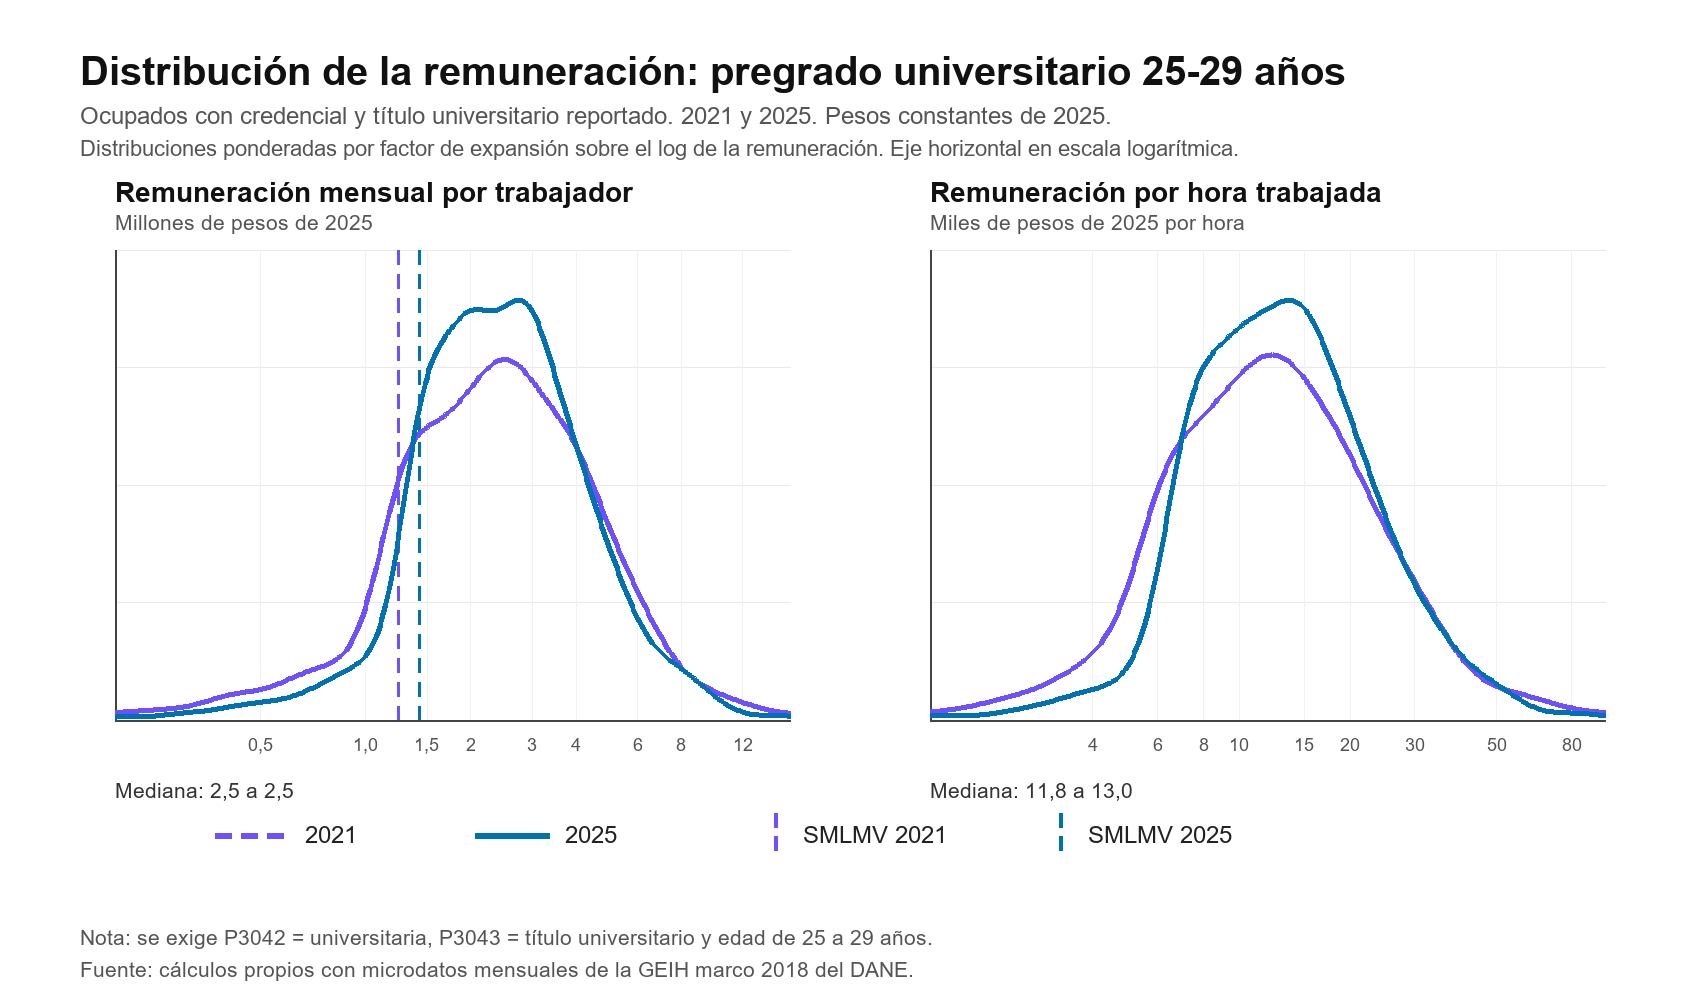
\includegraphics[width=0.98\textwidth]{Paper/figures/fig_kernel_pregrado_universitario_25_29_2021_2025.png}
%  \caption{Distribución de la remuneración laboral de ocupados de 25 a 29 años con pregrado universitario, 2021 y 2025}
  %\label{fig:kernel_pregrado_universitario_25_29}
  %\caption*{\footnotesize Fuente: cálculos propios con microdatos mensuales de la GEIH marco 2018 del DANE.}
%\end{figure}

\section{Conclusiones}\label{sec:conclusiones}

\textbf{El aumento del nivel educativo de la población ocupada explica una parte importante del crecimiento de la remuneración promedio observado en los últimos quince años.} La educación continúa estando estrechamente asociada con mejores resultados laborales y mayores ingresos. Sin embargo, los resultados de este informe muestran que el incremento de la remuneración promedio de los trabajadores ha estado impulsado principalmente por el creciente peso de los niveles educativos más altos dentro de la población ocupada, más que por aumentos significativos de la remuneración al interior de cada grupo educativo.

%\textbf{Para las personas, estudiar más sigue siendo una vía de movilidad, pero no sustituye una agenda de productividad.} Alcanzar un mayor logro educativo mejora la probabilidad de acceder a ocupaciones mejor remuneradas. Sin embargo, si la remuneración dentro de cada logro educativo crece lentamente, estudiar más puede mejorar la posición individual, pero no basta como estrategia agregada. El país necesita que más personas completen trayectorias educativas de calidad, y también que los empleos disponibles para cada logro educativo sean más productivos.

\textbf{El lento crecimiento de la remuneración de quienes alcanzaron educación superior constituye una señal que merece atención.} El análisis más detallado de los distintos niveles de educación superior muestra resultados heterogéneos. Entre 2021 y 2025, los trabajadores con doctorado, maestría, formación técnica profesional o formación tecnológica registraron aumentos reales en su remuneración. En contraste, quienes alcanzaron como máximo nivel educativo un pregrado universitario o una especialización experimentaron un estancamiento de sus ingresos o incluso reducciones reales. Comprender las razones detrás de este comportamiento representa una agenda relevante para futuras investigaciones sobre el mercado laboral colombiano.


% Bloque desactivado: conclusión asociada al material de edad y cohortes movido al apéndice.
\iffalse
\textbf{La comparación por edad y cohorte advierte que el promedio de cada logro educativo puede ocultar cambios internos.} En el grupo de educación superior, los grupos jóvenes tuvieron mayores remuneraciones reales en 2025 que los grupos de la misma edad en 2010, mientras los grupos de 45 años o más tuvieron remuneraciones menores. Al seguir cohortes de nacimiento comparables, la cohorte más joven muestra el mayor aumento de remuneración. La evidencia merece seguimiento porque puede reflejar cambios en la composición interna del grupo de educación superior, en las ocupaciones de destino o en la demanda relativa por experiencia.
\fi

%\textbf{La apertura de la pregunta educativa permite mirar mejor la heterogeneidad reciente.} Desde 2021, las categorías detalladas muestran diferencias entre técnica profesional, tecnológica, universitaria y posgrados, así como entre media académica y media técnica. Esa información puede aprovecharse en informes posteriores para conectar credenciales educativas con ocupaciones, sectores y calidad del empleo.

\textbf{La agenda de productividad del país debe seguir promoviendo mayores niveles de educación, pero también fortalecer la capacidad de generar ingresos dentro de cada nivel educativo.} Mantener el avance educativo de la población ocupada seguirá siendo fundamental para ampliar el acceso a empleos de mayor calidad y mejor remunerados. No obstante, los resultados sugieren que esta estrategia, por sí sola, no será suficiente para sostener mejoras significativas en los ingresos laborales. También será necesario impulsar aumentos de productividad que se traduzcan en mejores remuneraciones para los trabajadores de todos los niveles educativos. En particular, el desempeño reciente de los egresados universitarios pone de manifiesto la importancia de fortalecer la calidad y pertinencia de la educación superior, así como su articulación con las necesidades del sector productivo.

\clearpage
\appendix
\renewcommand{\thetable}{A\arabic{table}}
\renewcommand{\thefigure}{A\arabic{figure}}
\renewcommand{\theHtable}{appendix.table.\arabic{table}}
\renewcommand{\theHfigure}{appendix.figure.\arabic{figure}}
\setcounter{table}{0}
\setcounter{figure}{0}

\section{Cuadros y figuras de apoyo}\label{sec:apendice_cuadros}

% Bloque desactivado: esta figura correspondía a la agregación anterior de tres logros educativos.
\iffalse
\begin{figure}[H]
  \centering
  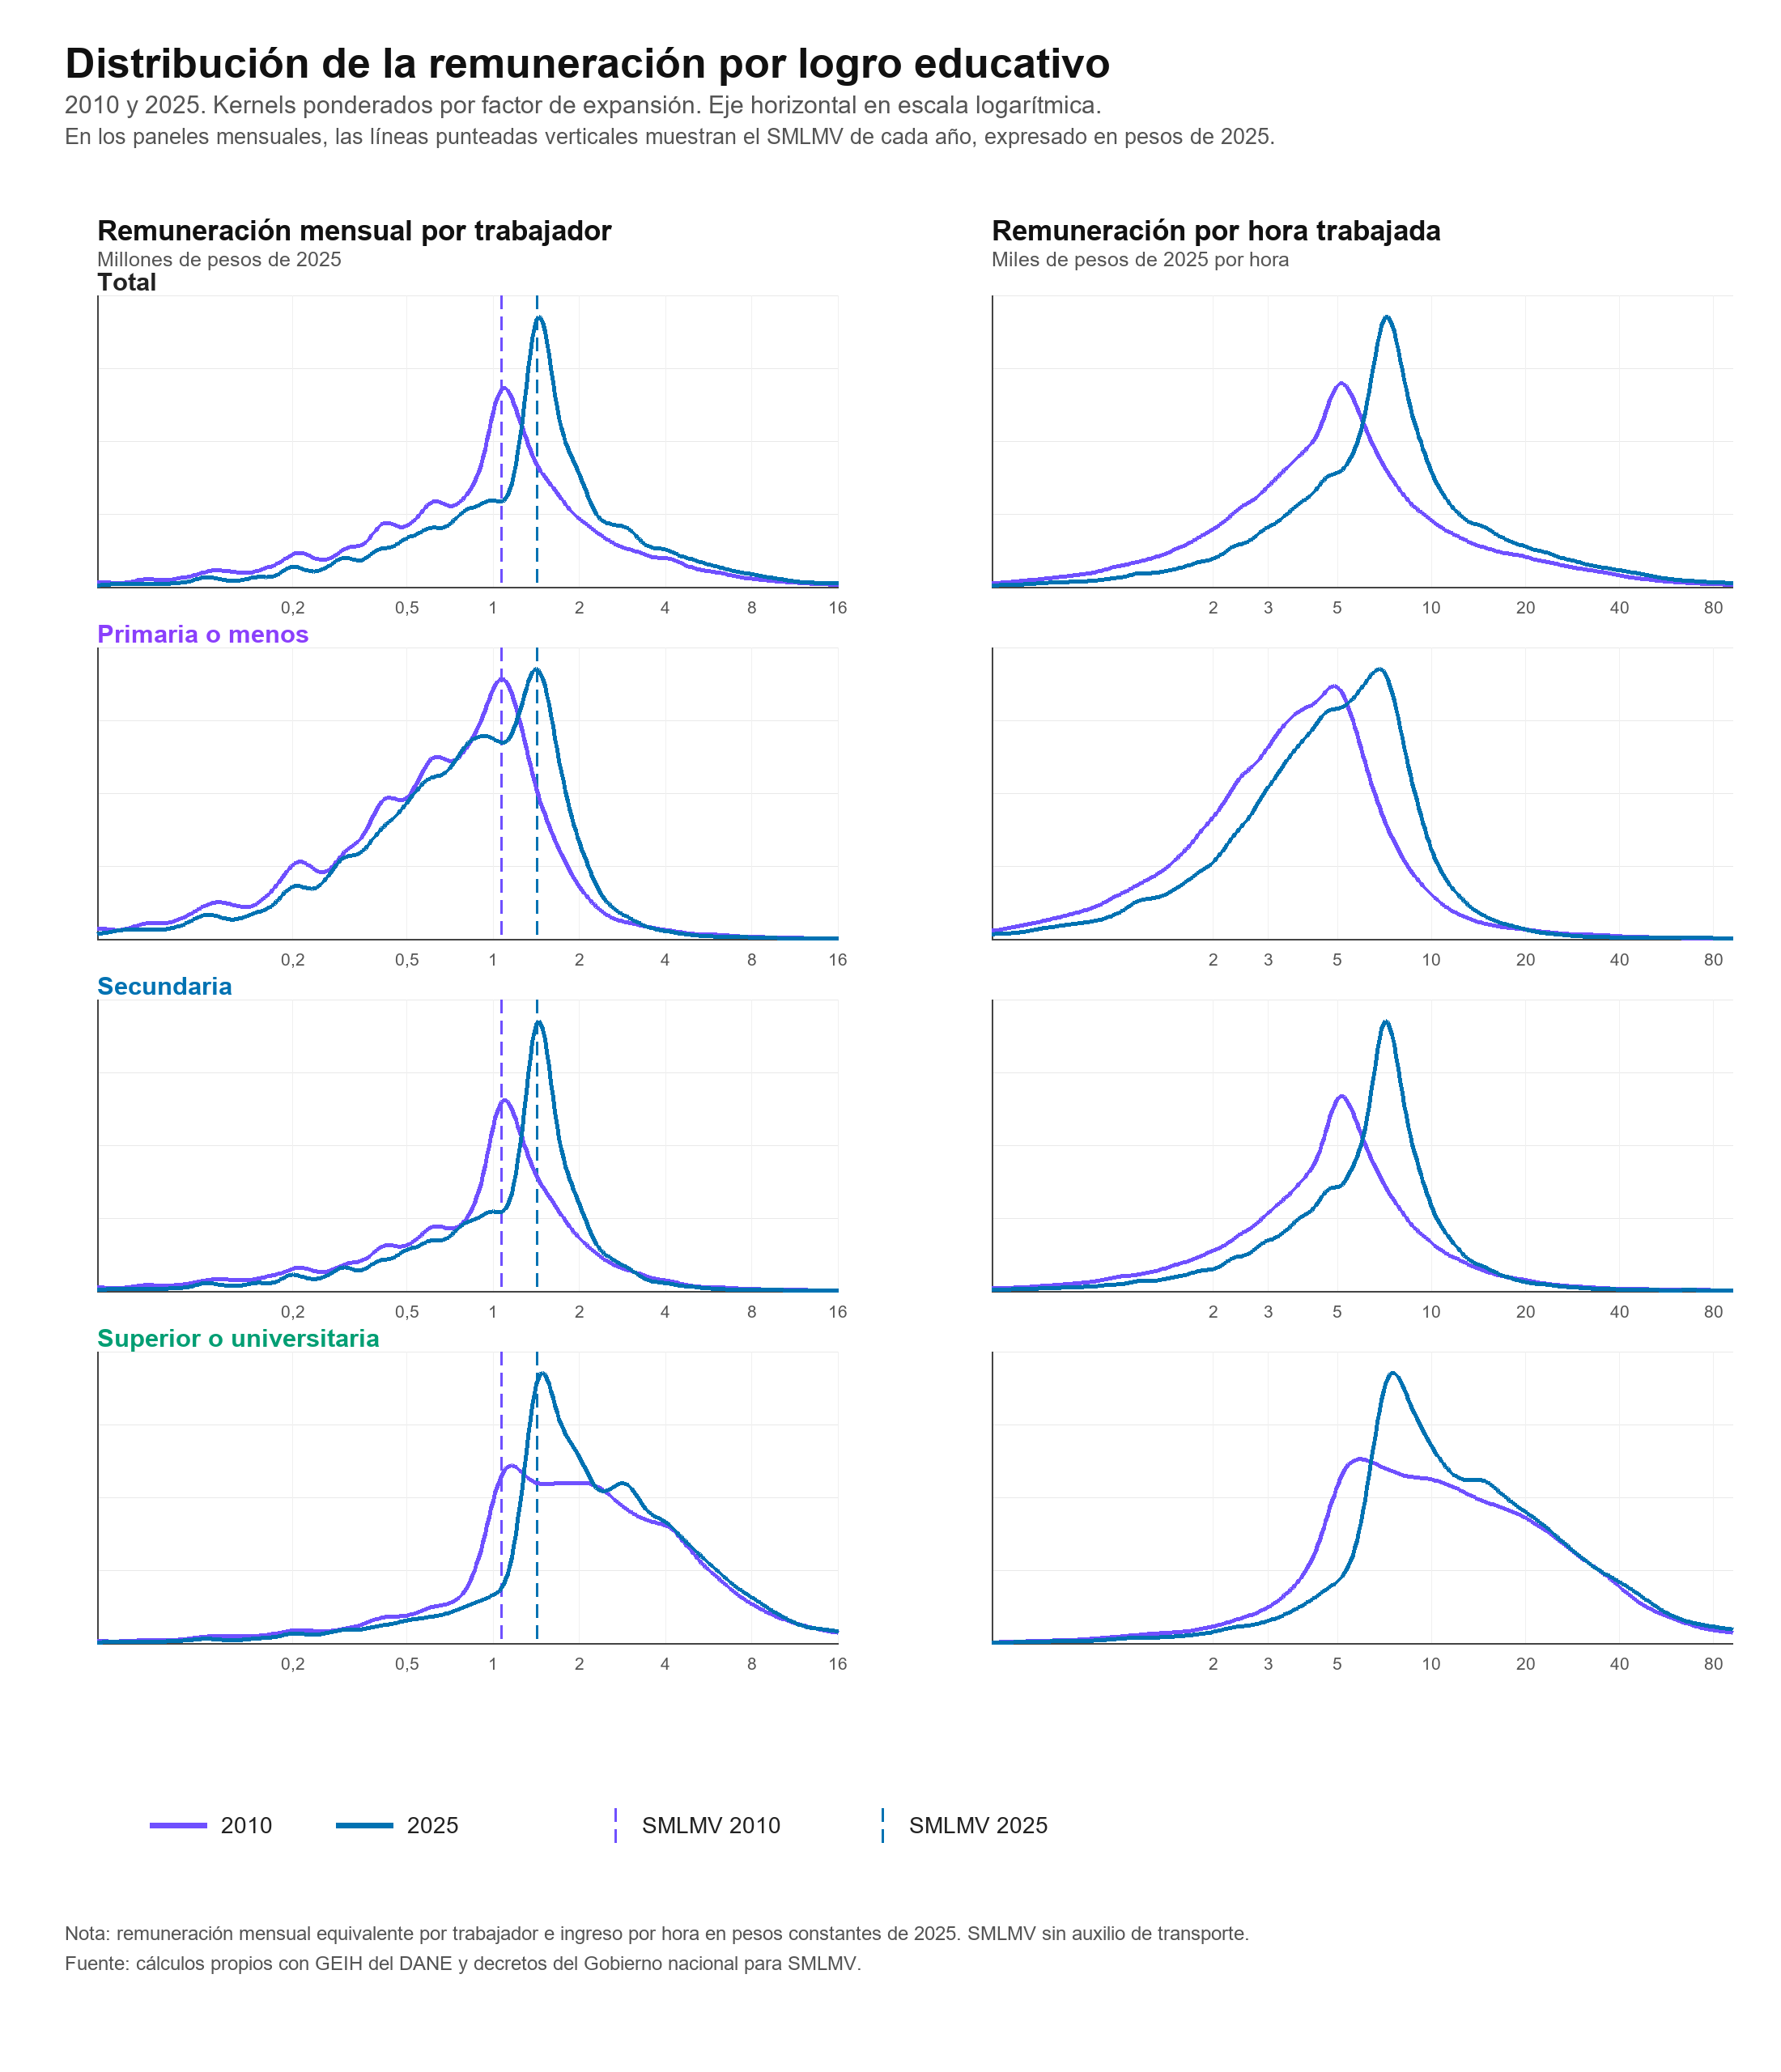
\includegraphics[width=0.98\textwidth]{Paper/figures/fig_kernel_remuneracion_educacion_comparable_2010_2025.png}
  \caption{Distribución de la remuneración laboral total y por logro educativo, 2010 y 2025}
  \label{fig:remuneracion_educacion_kernels}
  \caption*{\footnotesize Nota: distribuciones estimadas con factores de expansión. Los paneles mensuales muestran remuneración mensual equivalente por trabajador. Los paneles por hora muestran ingreso laboral por hora. El eje horizontal está en escala logarítmica. El SMLMV no incluye auxilio de transporte. Fuente: cálculos propios con GEIH del DANE y decretos del Gobierno nacional para SMLMV.}
\end{figure}
\fi

\begin{figure}[H]
  \centering
  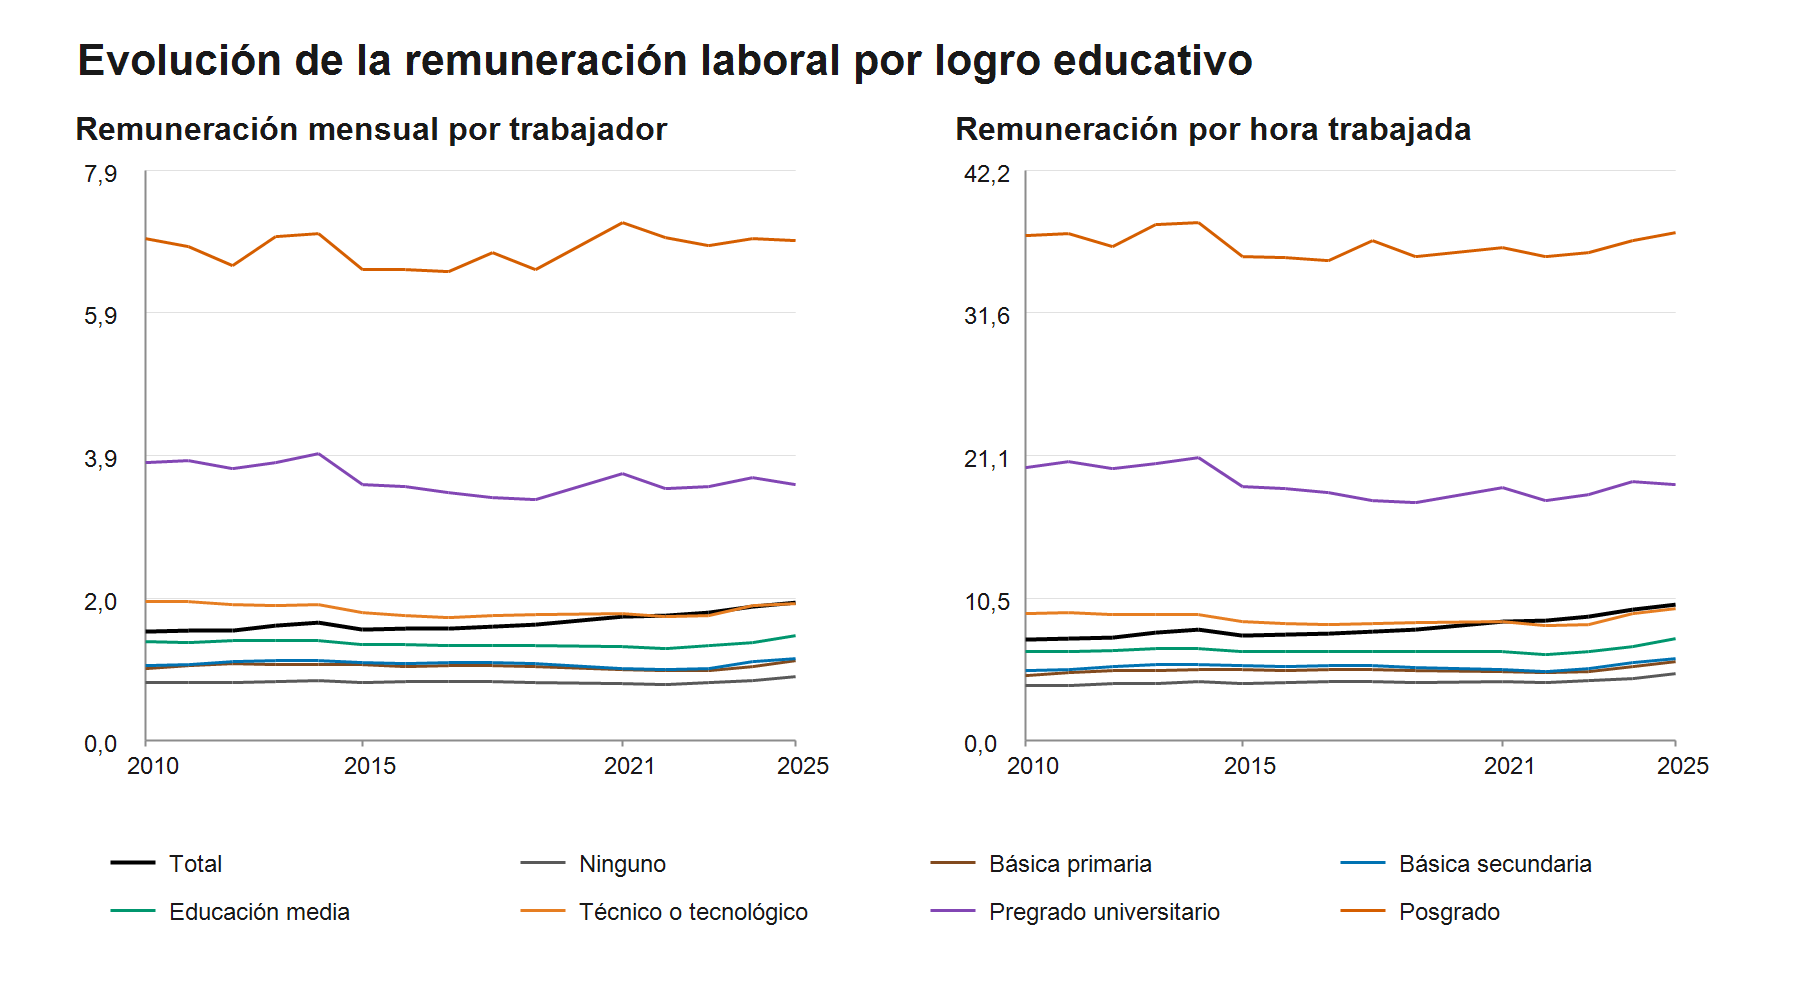
\includegraphics[width=0.98\textwidth]{Paper/figures/fig_remuneracion_educacion_series_comparables.png}
  \caption{Evolución de la remuneración laboral total y por logro educativo, 2010--2025}
  \label{fig:remuneracion_educacion_series_comparables}
  \caption*{\footnotesize Nota: el panel izquierdo muestra la remuneración mensual por trabajador en millones de pesos mensuales de 2025. El panel derecho muestra la remuneración por hora trabajada en miles de pesos de 2025. El eje vertical de ambos paneles está en escala logarítmica. La serie excluye 2020. Fuente: cálculos propios con GEIH del DANE.}
\end{figure}

% Bloque desactivado: este cuadro correspondía a la agregación anterior de tres logros educativos.
\iffalse
\begin{table}[H]
\centering
\caption{Tasas laborales por logro educativo comparable, 2010 y 2025}
\label{tab:tasas-laborales-educacion}
\begin{threeparttable}
\scriptsize
\setlength{\tabcolsep}{3.5pt}
\resizebox{\textwidth}{!}{%
\begin{tabular}{lcccccccc}
\toprule
& \multicolumn{2}{c}{Tasa de participación}
& \multicolumn{2}{c}{Tasa de ocupación}
& \multicolumn{2}{c}{Tasa de desempleo}
& \multicolumn{2}{c}{Tasa de formalidad} \\
\cmidrule(lr){2-3} \cmidrule(lr){4-5} \cmidrule(lr){6-7} \cmidrule(l){8-9}
Logro educativo
& 2010 & 2025
& 2010 & 2025
& 2010 & 2025
& 2010 & 2025 \\
\midrule
Primaria o menos
& 62,9 & 52,8
& 57,8 & 50,0
& 8,2 & 5,4
& 11,5 & 13,0 \\

Secundaria o media
& 67,1 & 64,1
& 57,4 & 57,8
& 14,4 & 9,6
& 31,3 & 36,7 \\

Superior o universitaria
& 78,3 & 74,3
& 67,9 & 67,0
& 13,3 & 10,0
& 67,5 & 76,0 \\
\bottomrule
\end{tabular}
}
\begin{tablenotes}
\scriptsize
\item \textit{Nota:} La tasa de participación se calcula como PEA/PET, la tasa de ocupación como ocupados/PET, la tasa de desempleo como desocupados/PEA y la tasa de formalidad como ocupados que cotizan a pensión sobre ocupados con clasificación válida de cotización. Las tasas se reportan en porcentaje. Los cálculos usan factores de expansión anualizados.
\end{tablenotes}
\end{threeparttable}
\end{table}
\fi

\begin{table}[H]
\centering
\caption{Tasas laborales por logro educativo detallado, 2021 y 2025}
\label{tab:tasas-laborales-educacion-detallada-2021-2025}
\begin{threeparttable}
\scriptsize
\setlength{\tabcolsep}{3.5pt}
\resizebox{\textwidth}{!}{%
\begin{tabular}{lccccccccc}
\toprule
& \multicolumn{3}{c}{Tasa de participación}
& \multicolumn{3}{c}{Tasa de ocupación}
& \multicolumn{3}{c}{Tasa de desempleo} \\
\cmidrule(lr){2-4} \cmidrule(lr){5-7} \cmidrule(lr){8-10}
Logro educativo
& 2021 & 2025 & Dif.
& 2021 & 2025 & Dif.
& 2021 & 2025 & Dif. \\
\midrule
Preescolar o ninguno
& 40,6 & 40,8 & 0,2
& 38,1 & 39,0 & 1,0
& 6,2 & 4,3 & -1,9 \\

Básica primaria
& 42,9 & 45,2 & 2,3
& 38,7 & 43,0 & 4,3
& 9,8 & 4,9 & -4,9 \\

Básica secundaria
& 53,4 & 55,4 & 2,0
& 48,7 & 52,4 & 3,7
& 9,0 & 5,5 & -3,4 \\

Media académica
& 51,3 & 55,1 & 3,8
& 43,9 & 50,3 & 6,4
& 14,5 & 8,7 & -5,8 \\

Media técnica
& 65,0 & 67,5 & 2,5
& 54,2 & 60,9 & 6,7
& 16,6 & 9,9 & -6,8 \\

Normalista
& 66,0 & 67,9 & 1,9
& 54,1 & 60,1 & 5,9
& 18,0 & 11,5 & -6,4 \\

Técnica profesional
& 51,5 & 50,7 & -0,8
& 42,9 & 42,5 & -0,4
& 16,7 & 16,1 & -0,6 \\

Tecnológica
& 74,1 & 74,0 & -0,1
& 60,6 & 65,3 & 4,6
& 18,2 & 11,8 & -6,4 \\

Universitaria
& 76,8 & 76,0 & -0,8
& 63,6 & 68,0 & 4,4
& 17,2 & 10,5 & -6,7 \\

Especialización
& 69,2 & 70,6 & 1,5
& 59,7 & 63,2 & 3,5
& 13,8 & 10,6 & -3,2 \\

Maestría
& 84,6 & 85,3 & 0,7
& 79,8 & 80,6 & 0,8
& 5,6 & 5,4 & -0,2 \\

Doctorado
& 89,4 & 90,1 & 0,7
& 85,8 & 86,4 & 0,5
& 4,0 & 4,2 & 0,2 \\
\bottomrule
\end{tabular}
}
\begin{tablenotes}
\scriptsize
\item \textit{Nota:} La tasa de participación se calcula como PEA/PET, la tasa de ocupación como ocupados/PET y la tasa de desempleo como desocupados/PEA. Las diferencias están expresadas en puntos porcentuales. Los cálculos usan factores de expansión anualizados.
\end{tablenotes}
\end{threeparttable}
\end{table}


% Bloque desactivado: no se referencia en el cuerpo del documento.
\iffalse
\begin{table}[H]
\centering
\caption{Estadísticos descriptivos de la remuneración laboral por logro educativo, 2010 y 2025}
\label{tab:estadisticos_remuneracion_educacion}
\begingroup
\setlength{\tabcolsep}{3.5pt}
\scriptsize
\begin{tabular}{@{}p{3.1cm}rrrrrr@{}}
\toprule
\multicolumn{7}{@{}l}{\textbf{Panel A. Remuneración mensual por trabajador (miles de pesos mensuales de 2025)}} \\
Logro educativo & Año & Media & Mediana & Desv. est. & Mín. & Máx. \\
\midrule
Primaria o menos & 2010 & 878 & 726 & 4.450 & $<1$ & 2.073.526 \\
Primaria o menos & 2025 & 997 & 850 & 989 & $<1$ & 80.000 \\
\addlinespace[0.25em]
Secundaria & 2010 & 1.195 & 1.068 & 1.491 & $<1$ & 207.311 \\
Secundaria & 2025 & 1.342 & 1.400 & 1.406 & $<1$ & 100.000 \\
\addlinespace[0.25em]
Superior o normalista & 2010 & 3.082 & 1.990 & 4.940 & $<1$ & 207.311 \\
Superior o normalista & 2025 & 3.228 & 2.000 & 3.921 & $<1$ & 103.000 \\
\addlinespace[0.8em]
\multicolumn{7}{@{}l}{\textbf{Panel B. Remuneración por hora trabajada (pesos de 2025 por hora)}} \\
Logro educativo & Año & Media & Mediana & Desv. est. & Mín. & Máx. \\
\midrule
Primaria o menos & 2010 & 4.561 & 3.615 & 17.679 & $<1$ & 7.975.098 \\
Primaria o menos & 2025 & 5.520 & 4.720 & 6.124 & $<1$ & 415.385 \\
\addlinespace[0.25em]
Secundaria & 2010 & 6.105 & 4.983 & 8.934 & $<1$ & 1.063.134 \\
Secundaria & 2025 & 7.106 & 6.827 & 8.151 & $<1$ & 1.153.846 \\
\addlinespace[0.25em]
Superior o normalista & 2010 & 17.042 & 10.229 & 28.960 & $<1$ & 1.794.038 \\
Superior o normalista & 2025 & 18.015 & 11.454 & 23.364 & $<1$ & 2.307.692 \\
\bottomrule
\end{tabular}
\endgroup
\caption*{\footnotesize Nota: media, mediana y desviación estándar se calculan con factores de expansión. Los mínimos y máximos son valores observados en la muestra y pueden estar afectados por valores extremos. Valores positivos menores a una unidad del panel se reportan como \(<1\). La media del Panel B describe el ingreso por hora promedio entre trabajadores. Por construcción, puede diferir de la remuneración por hora agregada del Cuadro \ref{tab:remuneracion_educacion_remuneracion}, que pondera por horas trabajadas. Fuente: cálculos propios con GEIH del DANE.}
\end{table}


\begin{table}[H]
\centering
\caption{Dispersión y masa alrededor del salario mínimo por logro educativo, 2010 y 2025}
\label{tab:masa_smlmv_educacion}
\begingroup
\setlength{\tabcolsep}{3.5pt}
\scriptsize
\begin{tabular}{@{}p{3.5cm}rrrrrr@{}}
\toprule
& \multicolumn{2}{c}{P90/P10 mensual} & \multicolumn{2}{c}{P90/P10 por hora} & \multicolumn{2}{c}{Cerca del SMLMV} \\
\cmidrule(lr){2-3} \cmidrule(lr){4-5} \cmidrule(l){6-7}
Logro educativo & 2010 & 2025 & 2010 & 2025 & 2010 & 2025 \\
\midrule
Primaria o menos & 9,2 & 7,2 & 6,3 & 5,2 & 14,2\% & 16,2\% \\
Secundaria o media & 8,3 & 5,0 & 5,4 & 4,0 & 21,0\% & 29,1\% \\
Superior o universitaria & 10,0 & 6,8 & 8,3 & 6,6 & 11,7\% & 18,4\% \\
\midrule
\textbf{Total} & 12,2 & 8,8 & 9,0 & 7,3 & 16,4\% & 22,8\% \\
\bottomrule
\end{tabular}
\endgroup
\caption*{\footnotesize Nota: cerca del SMLMV corresponde a la proporción de ocupados cuya remuneración mensual equivalente está entre 0,9 y 1,1 veces el salario mínimo legal mensual vigente del año, ambos expresados en pesos de 2025. Cálculos ponderados con factores de expansión. Fuente: cálculos propios con GEIH del DANE y decretos del Gobierno nacional para SMLMV.}
\end{table}

\fi

% Bloque desactivado: no se referencia en el cuerpo del documento.
\iffalse
\begin{figure}[H]
  \centering
  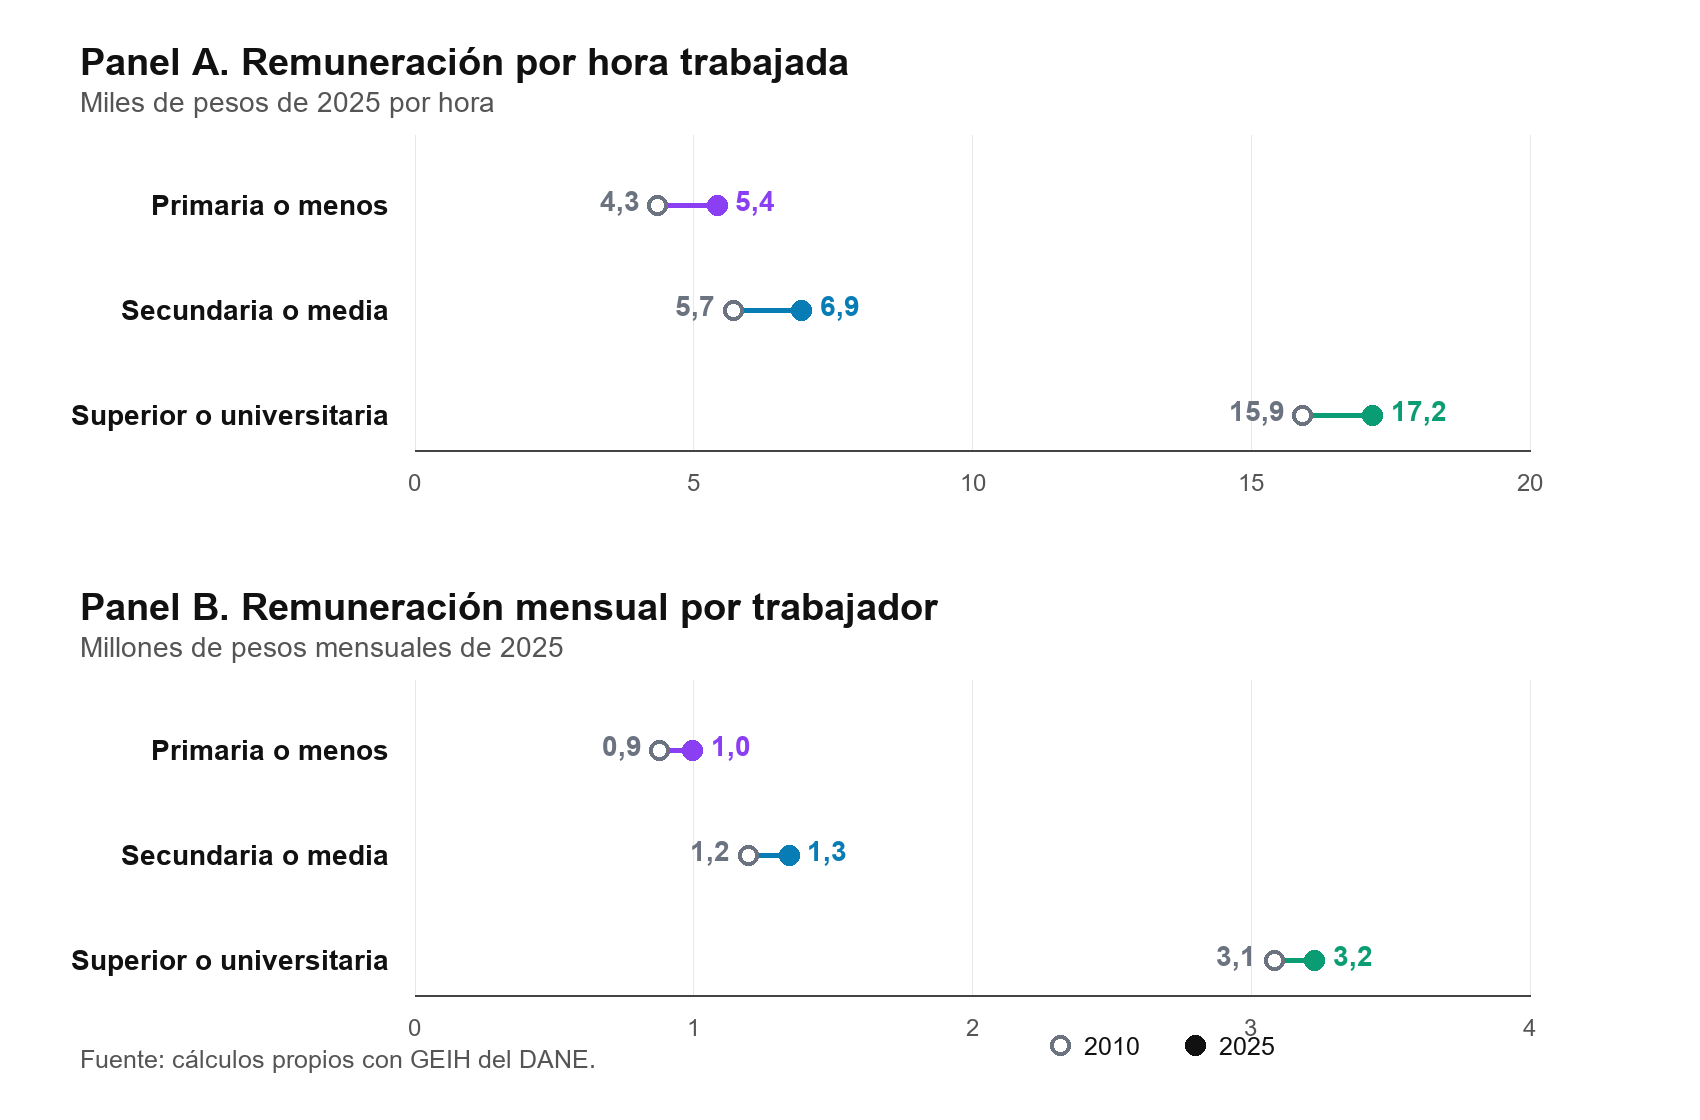
\includegraphics[width=0.98\textwidth]{Paper/figures/fig_remuneracion_educacion_niveles_2025.png}
  \caption{Remuneración laboral por logro educativo, 2010 y 2025}
  \label{fig:remuneracion_educacion_niveles_2025}
  \caption*{\footnotesize Nota: los círculos abiertos corresponden a 2010 y los círculos llenos a 2025. Pesos constantes de 2025. Fuente: cálculos propios con GEIH del DANE.}
\end{figure}
\fi

\begin{figure}[H]
  \centering
  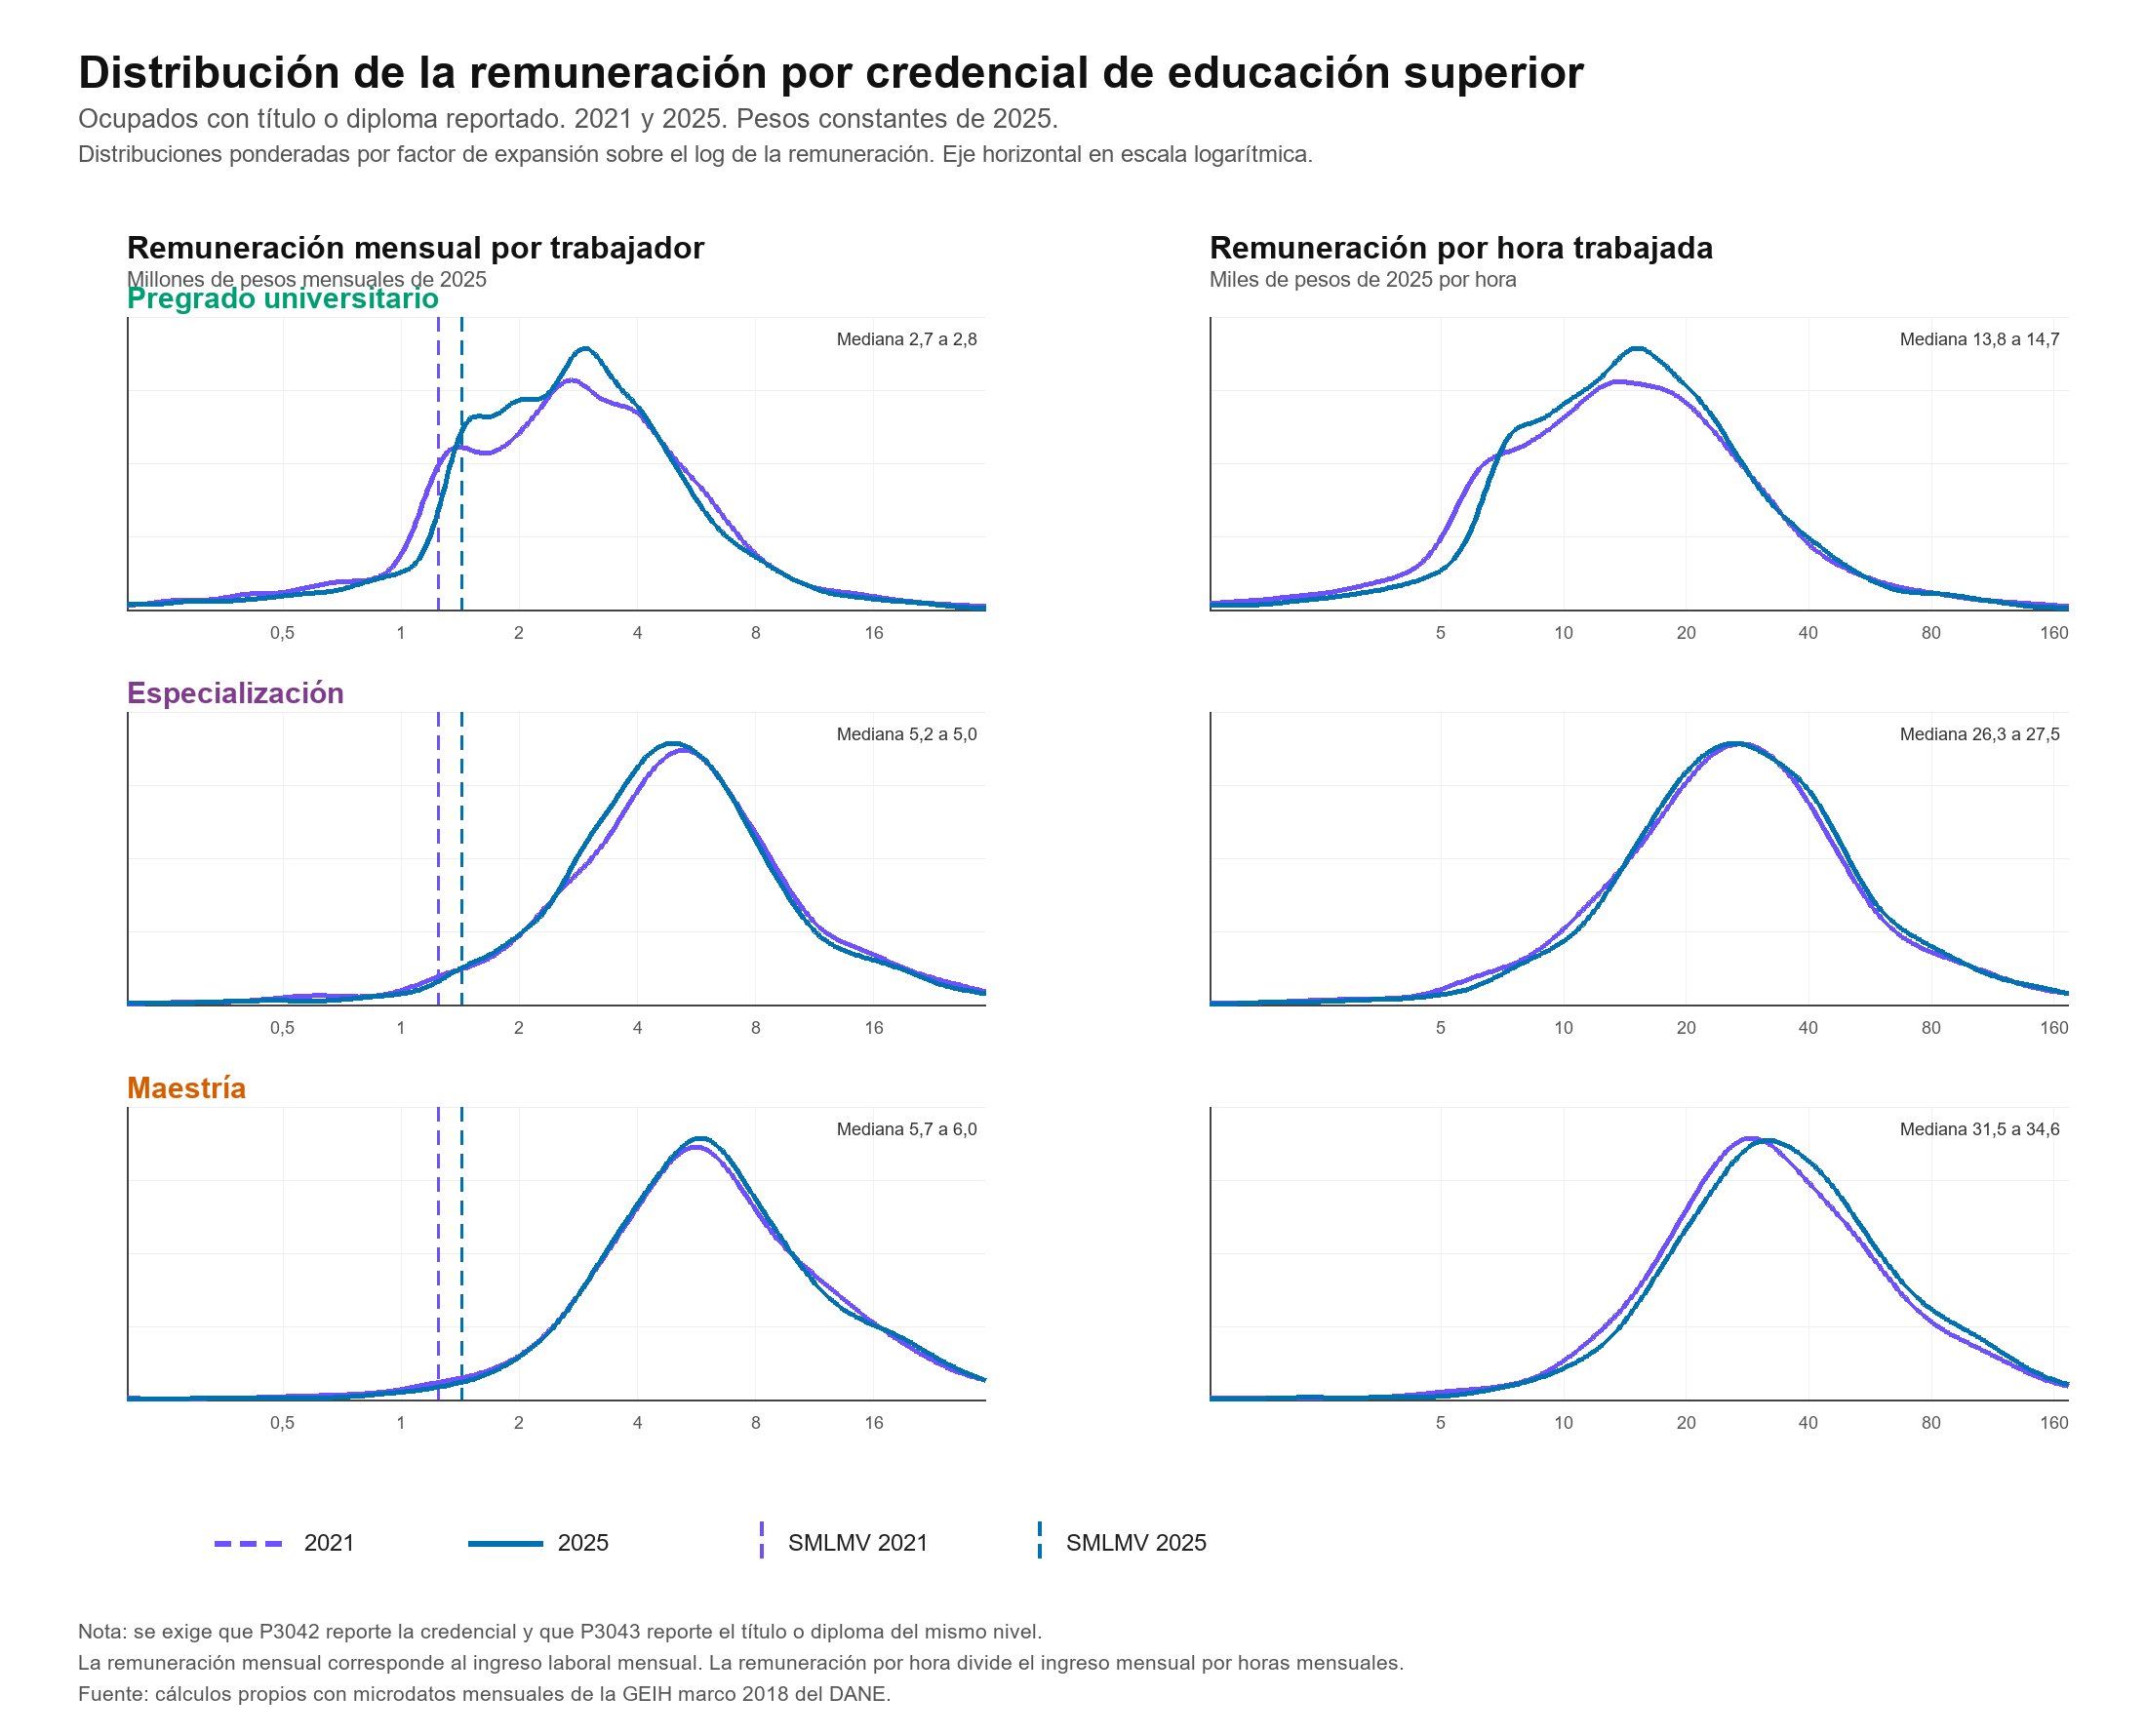
\includegraphics[width=0.98\textwidth]{Paper/figures/fig_kernel_remuneracion_credenciales_superiores_2021_2025.png}
  \caption{Distribución de la remuneración laboral por credencial de educación superior, 2021 y 2025}
  \label{fig:kernel_remuneracion_credenciales_superiores}
  \caption*{\footnotesize Nota: distribuciones estimadas con factores de expansión sobre el log de la remuneración. Se exige que P3042 reporte la credencial y que P3043 reporte el título o diploma del mismo nivel. El eje horizontal está en escala logarítmica. La remuneración mensual está en millones de pesos mensuales de 2025 y la remuneración por hora en miles de pesos de 2025 por hora. Fuente: cálculos propios con GEIH del DANE.}
\end{figure}

\begin{table}[H]
\centering
\caption{Aportes por logro educativo a la descomposición de la remuneración laboral, 2010--2025}
\label{tab:descomposicion_remuneracion_educacion_detalle}
\scriptsize
\begin{tabular}{@{}p{6.4cm}rr@{}}
\toprule
\multicolumn{3}{@{}l}{\textbf{Panel A. Remuneración mensual por trabajador}} \\
Factor & \shortstack{Aporte al cambio\\(miles de pesos\\mensuales de 2025)} & \shortstack{\% del\\cambio total} \\
\midrule
Productividad: Ninguno & 13,7 & 3,5\% \\
Productividad: Básica primaria & 23,6 & 6,0\% \\
Productividad: Básica secundaria & 5,1 & 1,3\% \\
Productividad: Educación media & 28,4 & 7,2\% \\
Productividad: Técnico o tecnológico & -2,2 & -0,6\% \\
Productividad: Pregrado universitario & -29,3 & -7,4\% \\
Productividad: Posgrado & -1,1 & -0,3\% \\
\textbf{Total productividad} & \textbf{38,1} & \textbf{9,6\%} \\
\addlinespace[0.35em]
Logro educativo: Ninguno & -88,9 & -22,5\% \\
Logro educativo: Básica primaria & -91,6 & -23,2\% \\
Logro educativo: Básica secundaria & -16,4 & -4,1\% \\
Logro educativo: Educación media & 113,4 & 28,7\% \\
Logro educativo: Técnico o tecnológico & 107,0 & 27,0\% \\
Logro educativo: Pregrado universitario & 174,1 & 44,0\% \\
Logro educativo: Posgrado & 160,0 & 40,4\% \\
\textbf{Total logro educativo} & \textbf{357,6} & \textbf{90,4\%} \\
\addlinespace[0.35em]
\addlinespace[0.6em]
\multicolumn{3}{@{}l}{\textbf{Panel B. Remuneración por hora trabajada}} \\
Factor & \shortstack{Aporte al cambio\\(pesos de 2025\\por hora)} & \shortstack{\% del\\cambio total} \\
\midrule
Productividad: Ninguno & 136 & 5,2\% \\
Productividad: Básica primaria & 234 & 8,9\% \\
Productividad: Básica secundaria & 45 & 1,7\% \\
Productividad: Educación media & 319 & 12,2\% \\
Productividad: Técnico o tecnológico & 41 & 1,6\% \\
Productividad: Pregrado universitario & -117 & -4,5\% \\
Productividad: Posgrado & 9 & 0,3\% \\
\textbf{Total productividad} & \textbf{669} & \textbf{25,6\%} \\
\addlinespace[0.35em]
Logro educativo: Ninguno & -474 & -18,1\% \\
Logro educativo: Básica primaria & -499 & -19,1\% \\
Logro educativo: Básica secundaria & -83 & -3,2\% \\
Logro educativo: Educación media & 566 & 21,6\% \\
Logro educativo: Técnico o tecnológico & 561 & 21,4\% \\
Logro educativo: Pregrado universitario & 978 & 37,4\% \\
Logro educativo: Posgrado & 898 & 34,3\% \\
\textbf{Total logro educativo} & \textbf{1.946} & \textbf{74,4\%} \\
\addlinespace[0.35em]
\bottomrule
\end{tabular}
\caption*{\footnotesize Nota: los aportes al cambio preservan el signo de cada contribución. Los porcentajes dividen cada factor por el cambio total del indicador correspondiente. Fuente: cálculos propios con GEIH del DANE.}
\end{table}


% Bloque desactivado: no se referencia en el cuerpo del documento.
\iffalse
\begin{table}[H]
\centering
\caption{Composición de los ocupados por logro educativo, sexo y formalidad, 2010 y 2025}
\label{tab:composicion_educacion_sexo_formalidad}
\footnotesize
\begin{tabular}{@{}p{4.2cm}rrrr@{}}
\toprule
\multicolumn{5}{@{}l}{\textbf{Panel A. Sexo}} \\
Logro educativo & Hombre 2010 & Mujer 2010 & Hombre 2025 & Mujer 2025 \\
\midrule
Primaria o menos & 67,8\% & 32,2\% & 70,0\% & 30,0\% \\
Secundaria o media & 59,7\% & 40,3\% & 61,7\% & 38,3\% \\
Superior o universitaria & 48,5\% & 51,5\% & 47,9\% & 52,1\% \\
\textbf{Total} & 60,1\% & 39,9\% & 58,8\% & 41,2\% \\
\addlinespace[0.6em]
\multicolumn{5}{@{}l}{\textbf{Panel B. Formalidad}} \\
Logro educativo & Formal 2010 & Informal 2010 & Formal 2025 & Informal 2025 \\
\midrule
Primaria o menos & 11,5\% & 88,5\% & 13,0\% & 87,0\% \\
Secundaria o media & 31,3\% & 68,7\% & 36,7\% & 63,3\% \\
Superior o universitaria & 67,5\% & 32,5\% & 76,0\% & 24,0\% \\
\textbf{Total} & 32,4\% & 67,6\% & 44,9\% & 55,1\% \\
\bottomrule
\end{tabular}
\caption*{\footnotesize Nota: participaciones dentro de cada logro educativo, calculadas con factores de expansión sobre la misma submuestra usada para medir remuneración. El Panel B clasifica como formal a quienes cotizan a pensión e informal a quienes no cotizan. Excluye observaciones sin clasificación formal/informal válida. Fuente: cálculos propios con GEIH del DANE.}
\end{table}
\fi

% Bloque desactivado: no se referencia en el cuerpo del documento.
\iffalse
\begin{table}[H]
\centering
\caption{Remuneración laboral por logro educativo y formalidad, 2010 y 2025}
\label{tab:remuneracion_educacion_formalidad}
\footnotesize
\begin{tabular}{@{}p{4.0cm}rrrr@{}}
\toprule
\multicolumn{5}{@{}l}{\textbf{Panel A. Remuneración mensual por trabajador (millones de pesos mensuales de 2025)}} \\
Logro educativo & Formal 2010 & Informal 2010 & Formal 2025 & Informal 2025 \\
\midrule
Primaria o menos & 1,43 & 0,80 & 1,71 & 0,89 \\
Secundaria & 1,62 & 0,99 & 1,79 & 1,08 \\
Universitaria o superior & 3,65 & 1,85 & 3,73 & 1,49 \\
\textbf{Total} & 2,55 & 1,00 & 2,89 & 1,08 \\
\addlinespace[0.7em]
\multicolumn{5}{@{}l}{\textbf{Panel B. Remuneración por hora trabajada (miles de pesos de 2025 por hora)}} \\
Logro educativo & Formal 2010 & Informal 2010 & Formal 2025 & Informal 2025 \\
\midrule
Primaria o menos & 6,1 & 4,1 & 8,1 & 4,9 \\
Secundaria & 7,1 & 4,9 & 8,7 & 5,8 \\
Universitaria o superior & 18,0 & 10,4 & 19,2 & 8,7 \\
\textbf{Total} & 11,8 & 5,1 & 14,5 & 5,9 \\
\bottomrule
\end{tabular}
\caption*{\footnotesize Nota: la clasificación formal corresponde a trabajadores ocupados que cotizan a pensión. La clasificación informal corresponde a quienes no cotizan. El cuadro excluye observaciones sin clasificación formal o informal válida. Fuente: cálculos propios con GEIH del DANE.}
\end{table}

\fi

% Bloque desactivado: no se referencia en el cuerpo del documento.
\iffalse
\begin{table}[H]
\centering
\caption{Remuneración laboral por logro educativo y grupo de edad, 2010 y 2025}
\label{tab:remuneracion_educacion_cohorte}
\scriptsize
\begin{tabular}{@{}p{3.6cm}p{1.6cm}rrr@{}}
\toprule
\multicolumn{5}{@{}l}{\textbf{Panel A. Remuneración mensual por trabajador (millones de pesos mensuales de 2025)}} \\
Logro educativo & Edad & 2010 & 2025 & Crec. anual \\
\midrule
Primaria o menos & 15--24 & 0,7 & 0,9 & 1,8\% \\
Primaria o menos & 25--34 & 0,9 & 1,0 & 0,9\% \\
Primaria o menos & 35--44 & 0,9 & 1,1 & 0,9\% \\
Primaria o menos & 45--54 & 0,9 & 1,1 & 1,2\% \\
Primaria o menos & 55 o más & 0,8 & 0,9 & 0,5\% \\
\addlinespace[0.3em]
Secundaria & 15--24 & 0,9 & 1,1 & 1,8\% \\
Secundaria & 25--34 & 1,2 & 1,4 & 1,0\% \\
Secundaria & 35--44 & 1,3 & 1,4 & 0,5\% \\
Secundaria & 45--54 & 1,4 & 1,4 & 0,2\% \\
Secundaria & 55 o más & 1,5 & 1,3 & -0,9\% \\
\addlinespace[0.3em]
Universitaria o superior & 15--24 & 1,3 & 1,6 & 1,2\% \\
Universitaria o superior & 25--34 & 2,6 & 2,7 & 0,2\% \\
Universitaria o superior & 35--44 & 3,5 & 3,7 & 0,3\% \\
Universitaria o superior & 45--54 & 4,4 & 4,0 & -0,6\% \\
Universitaria o superior & 55 o más & 4,8 & 4,1 & -1,1\% \\
\addlinespace[0.7em]
\multicolumn{5}{@{}l}{\textbf{Panel B. Remuneración por hora trabajada (miles de pesos de 2025 por hora)}} \\
Logro educativo & Edad & 2010 & 2025 & Crec. anual \\
\midrule
Primaria o menos & 15--24 & 3,4 & 4,8 & 2,3\% \\
Primaria o menos & 25--34 & 4,3 & 5,4 & 1,5\% \\
Primaria o menos & 35--44 & 4,5 & 5,6 & 1,5\% \\
Primaria o menos & 45--54 & 4,4 & 5,8 & 1,8\% \\
Primaria o menos & 55 o más & 4,4 & 5,1 & 1,0\% \\
\addlinespace[0.3em]
Secundaria & 15--24 & 4,4 & 6,1 & 2,2\% \\
Secundaria & 25--34 & 5,4 & 6,9 & 1,7\% \\
Secundaria & 35--44 & 6,1 & 7,2 & 1,1\% \\
Secundaria & 45--54 & 6,5 & 7,2 & 0,7\% \\
Secundaria & 55 o más & 7,8 & 7,3 & -0,5\% \\
\addlinespace[0.3em]
Universitaria o superior & 15--24 & 7,4 & 9,1 & 1,4\% \\
Universitaria o superior & 25--34 & 13,1 & 14,1 & 0,5\% \\
Universitaria o superior & 35--44 & 17,8 & 19,0 & 0,5\% \\
Universitaria o superior & 45--54 & 23,0 & 21,3 & -0,5\% \\
Universitaria o superior & 55 o más & 27,2 & 23,4 & -1,0\% \\
\bottomrule
\end{tabular}
\caption*{\footnotesize Nota: el crecimiento es anualizado para 2010--2025. Los grupos de edad comparan personas del mismo rango etario observadas en cada año. No siguen una misma cohorte de nacimiento a lo largo del tiempo. Fuente: cálculos propios con GEIH del DANE.}
\end{table}


\begin{table}[H]
\centering
\caption{Remuneración laboral por cohorte de nacimiento y logro educativo, 2010 y 2025}
\label{tab:remuneracion_educacion_cohortes_nacimiento}
\scriptsize
\begin{tabular}{@{}p{2.0cm}p{3.5cm}rrr@{}}
\toprule
\multicolumn{5}{@{}l}{\textbf{Panel A. Remuneración mensual por trabajador (millones de pesos mensuales de 2025)}} \\
Cohorte & Logro educativo & 2010 & 2025 & Crec. anual \\
\midrule
1985--1990 & \textbf{Total} & 1,16 & 2,26 & 4,54\% \\
1985--1990 & Primaria o menos & 0,75 & 1,08 & 2,49\% \\
1985--1990 & Secundaria & 1,03 & 1,40 & 2,05\% \\
1985--1990 & Universitaria o superior & 1,63 & 3,69 & 5,61\% \\
\addlinespace[0.4em]
1980--1985 & \textbf{Total} & 1,52 & 2,22 & 2,58\% \\
1980--1985 & Primaria o menos & 0,85 & 1,06 & 1,54\% \\
1980--1985 & Secundaria & 1,15 & 1,44 & 1,51\% \\
1980--1985 & Universitaria o superior & 2,48 & 3,82 & 2,92\% \\
\addlinespace[0.4em]
1975--1980 & \textbf{Total} & 1,67 & 2,17 & 1,77\% \\
1975--1980 & Primaria o menos & 0,97 & 1,11 & 0,90\% \\
1975--1980 & Secundaria & 1,21 & 1,42 & 1,07\% \\
1975--1980 & Universitaria o superior & 3,02 & 4,11 & 2,07\% \\
\addlinespace[0.8em]
\multicolumn{5}{@{}l}{\textbf{Panel B. Remuneración por hora trabajada (miles de pesos de 2025 por hora)}} \\
Cohorte & Logro educativo & 2010 & 2025 & Crec. anual \\
\midrule
1985--1990 & \textbf{Total} & 5,7 & 11,6 & 4,87\% \\
1985--1990 & Primaria o menos & 3,6 & 5,7 & 3,02\% \\
1985--1990 & Secundaria & 4,9 & 7,0 & 2,52\% \\
1985--1990 & Universitaria o superior & 8,6 & 19,2 & 5,49\% \\
\addlinespace[0.4em]
1980--1985 & \textbf{Total} & 7,2 & 11,5 & 3,12\% \\
1980--1985 & Primaria o menos & 4,1 & 5,6 & 2,22\% \\
1980--1985 & Secundaria & 5,3 & 7,3 & 2,15\% \\
1980--1985 & Universitaria o superior & 12,4 & 19,9 & 3,19\% \\
\addlinespace[0.4em]
1975--1980 & \textbf{Total} & 8,0 & 11,3 & 2,34\% \\
1975--1980 & Primaria o menos & 4,7 & 5,8 & 1,49\% \\
1975--1980 & Secundaria & 5,6 & 7,3 & 1,73\% \\
1975--1980 & Universitaria o superior & 15,1 & 21,6 & 2,44\% \\
\bottomrule
\end{tabular}
\caption*{\footnotesize Nota: los rangos de cohorte son intervalos de cinco años. Por ejemplo, 1985--1990 incluye nacidos de 1985 a 1989. Se reportan las cohortes que aparecen tanto en 2010 como en 2025 dentro de los rangos solicitados. El crecimiento es anualizado para 2010--2025. Fuente: cálculos propios con GEIH del DANE.}
\end{table}

\fi

% Bloque desactivado: no se referencia en el cuerpo del documento.
\iffalse
\begin{table}[H]
\centering
\caption{Remuneración laboral de ocupados de 25 a 29 años con educación universitaria o superior, 2010 y 2025}
\label{tab:remuneracion_recien_graduados}
\footnotesize
\begin{tabular}{@{}p{6.6cm}rrr@{}}
\toprule
Indicador & 2010 & 2025 & Crec. anual \\
\midrule
Ocupados (millones de personas) & 0,73 & 1,27 & 3,73\% \\
Remuneración mensual por trabajador (millones de pesos de 2025) & 2,33 & 2,40 & 0,18\% \\
Remuneración por hora trabajada (miles de pesos de 2025) & 11,7 & 12,7 & 0,51\% \\
\bottomrule
\end{tabular}
\caption*{\footnotesize Nota: la GEIH no identifica si la persona acaba de graduarse ni el año de graduación. Este cuadro aproxima la remuneración de recién graduados con personas ocupadas de 25 a 29 años que reportan educación universitaria o superior. Por lo tanto, debe leerse como una aproximación a jóvenes con educación superior, no como graduados observados directamente. El crecimiento es anualizado para 2010--2025. La serie excluye 2020. Fuente: cálculos propios con GEIH del DANE.}
\end{table}

\fi

% Bloque desactivado: no se referencia en el cuerpo del documento.
\iffalse
\begin{figure}[H]
  \centering
  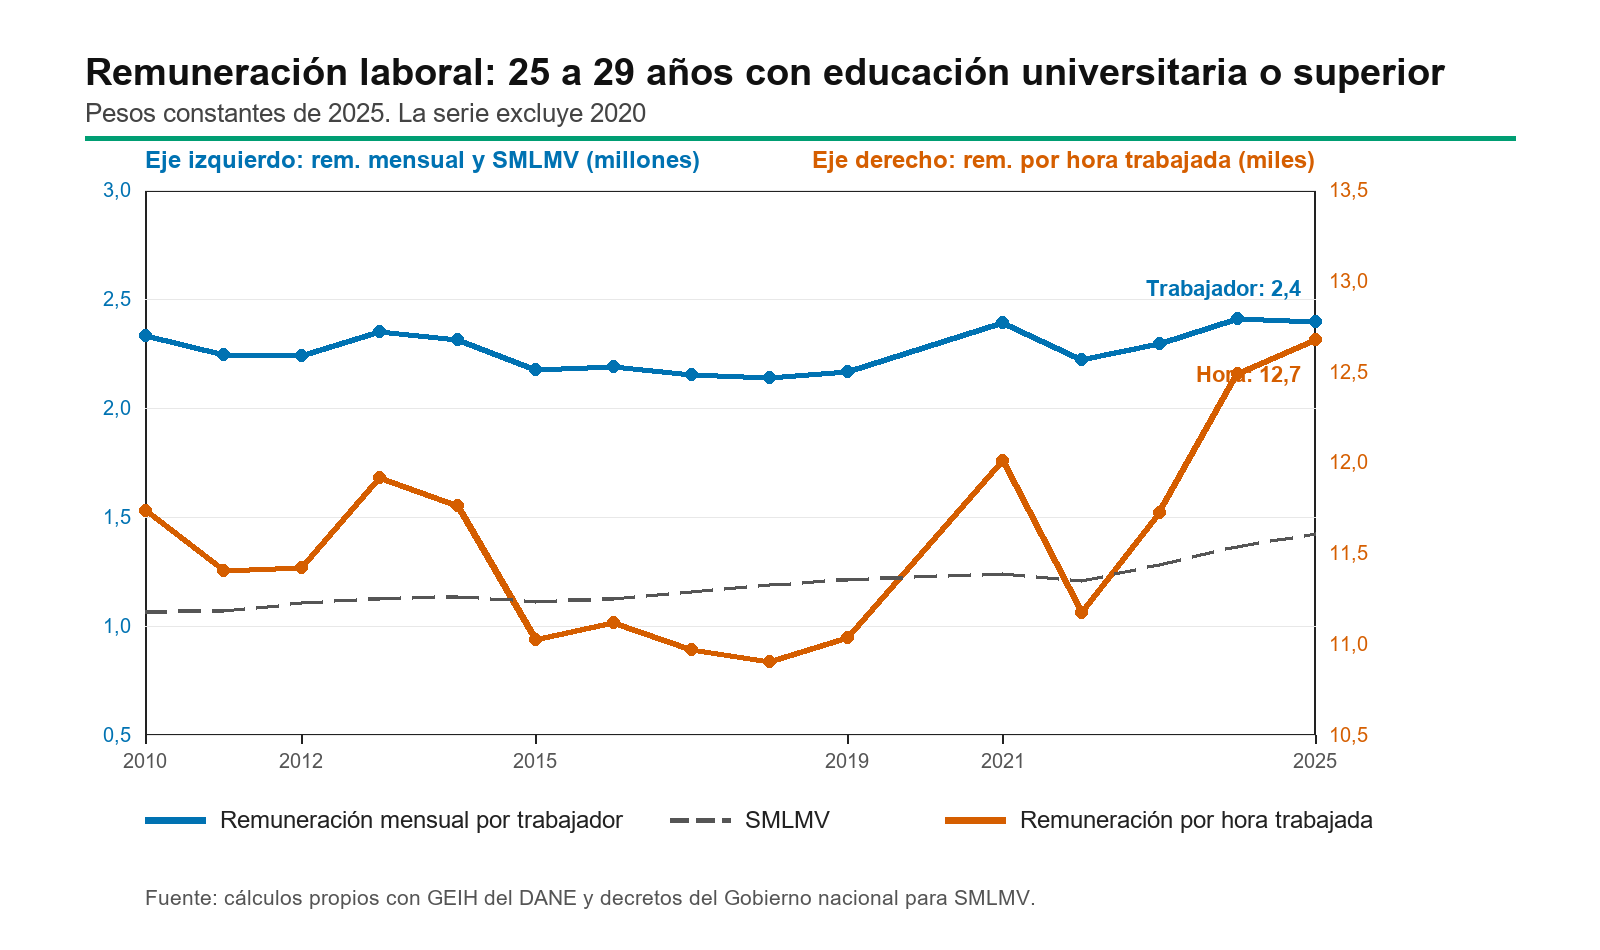
\includegraphics[width=0.96\textwidth]{Paper/figures/fig_remuneracion_recien_graduados_series.png}
  \caption{Evolución de la remuneración laboral de ocupados de 25 a 29 años con educación superior, 2010--2025}
  \label{fig:remuneracion_recien_graduados_series}
  \caption*{\footnotesize Nota: el eje izquierdo muestra la remuneración mensual por trabajador y el SMLMV, ambos en millones de pesos mensuales de 2025. El eje derecho muestra la remuneración por hora trabajada en miles de pesos de 2025. La GEIH no identifica si la persona acaba de graduarse ni el año de graduación. El grupo de 25 a 29 años con educación superior se usa como aproximación a recién graduados. El SMLMV no incluye auxilio de transporte. La serie excluye 2020. Fuente: cálculos propios con GEIH del DANE y decretos del Gobierno nacional para SMLMV.}
\end{figure}
\fi

% Bloque desactivado: no se referencia en el cuerpo del documento.
\iffalse
\begin{figure}[H]
  \centering
  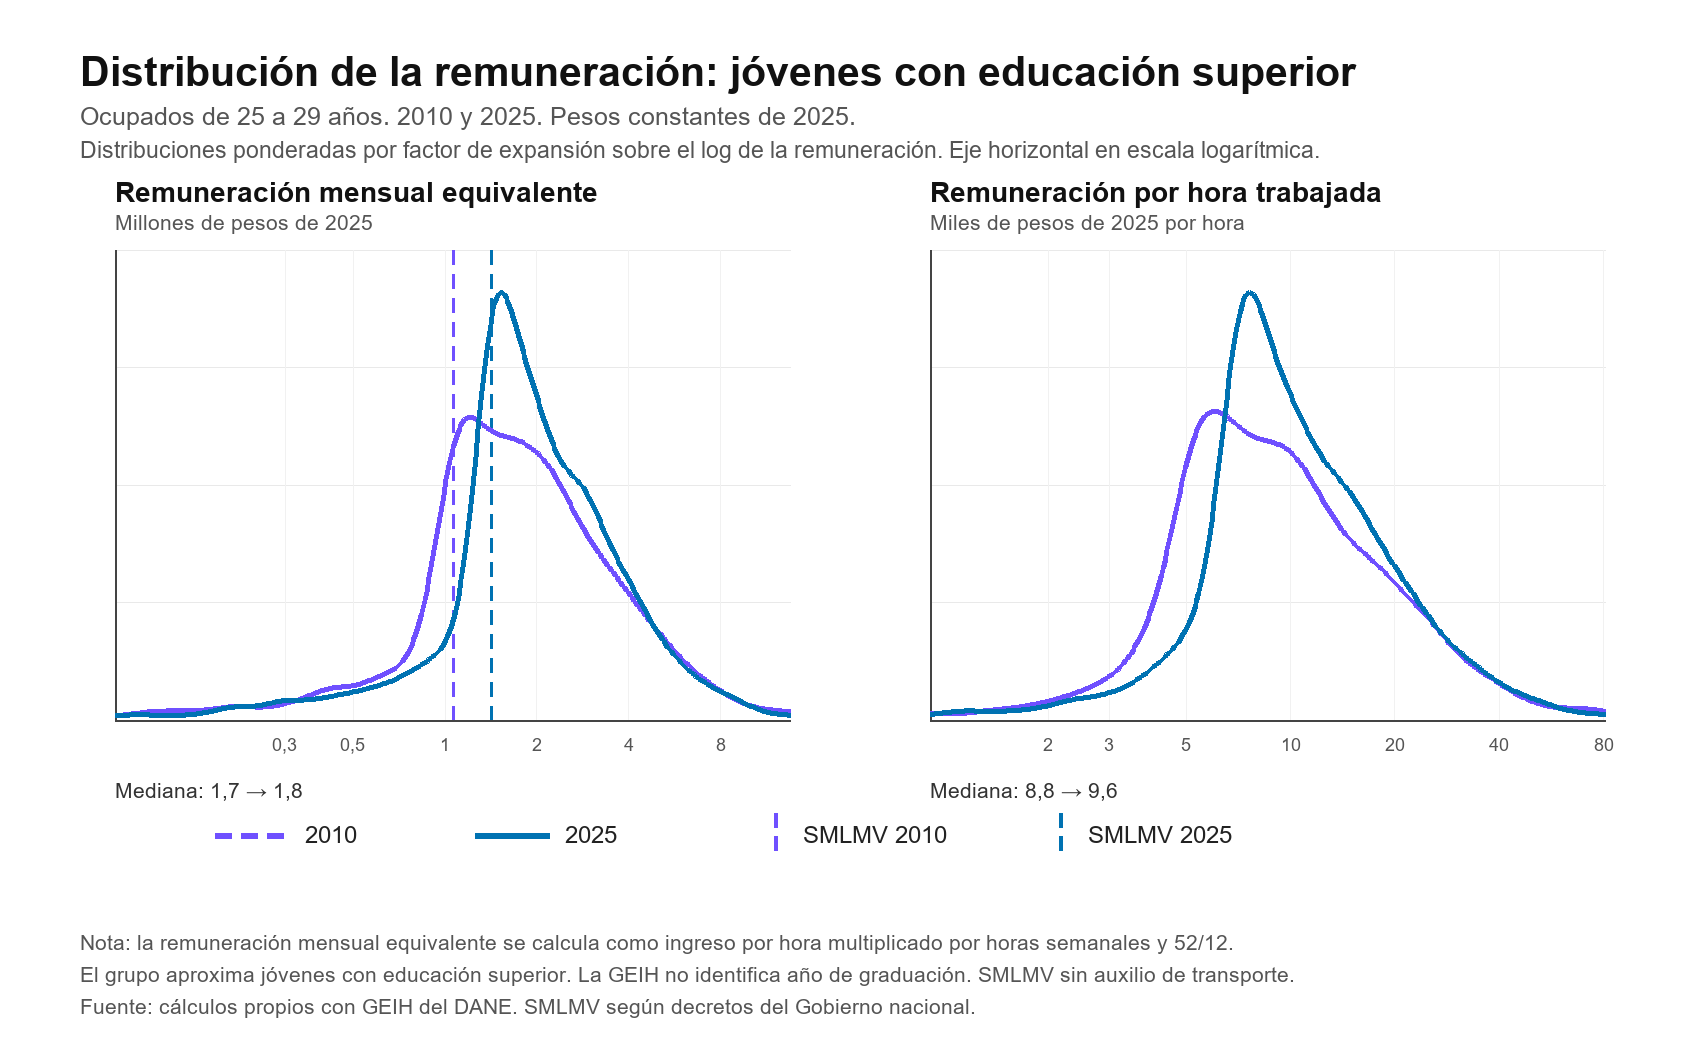
\includegraphics[width=0.98\textwidth]{Paper/figures/fig_kernel_remuneracion_universitaria_25_29_2010_2025.png}
  \caption{Distribución de la remuneración laboral de ocupados de 25 a 29 años con educación superior, 2010 y 2025}
  \label{fig:kernel_remuneracion_universitaria_25_29}
  \caption*{\footnotesize Nota: distribuciones estimadas con factores de expansión sobre el log de la remuneración. El eje horizontal está en escala logarítmica. La GEIH no identifica si la persona acaba de graduarse ni el año de graduación. El grupo de 25 a 29 años con educación superior se usa como aproximación a recién graduados. El SMLMV no incluye auxilio de transporte. Fuente: cálculos propios con GEIH del DANE y decretos del Gobierno nacional para SMLMV.}
\end{figure}
\fi



\end{document}
